\documentclass[11pt,letterpaper]{article}

\newenvironment{proof}{\noindent{\bf Proof:}}{\qed\bigskip}

\newtheorem{theorem}{Theorem}
\newtheorem{corollary}{Corollary}
\newtheorem{lemma}{Lemma} 
\newtheorem{claim}{Claim}
\newtheorem{fact}{Fact}
\newtheorem{definition}{Definition}
\newtheorem{assumption}{Assumption}
\newtheorem{observation}{Observation}
\newtheorem{example}{Example}
\newcommand{\qed}{\rule{7pt}{7pt}}

\newcommand{\solution}[4]{
\thispagestyle{plain} 
\newpage
\setcounter{page}{1}
\noindent
\begin{center}
\framebox{ \vbox{
\vspace{4mm}
\vspace{0.2in} 
{\centering \large\mbox{#3}}\\
\vspace{0.1in}
{#1 \hfill {Date: #2}}
}}
\end{center}
\markright{#1}
}

\newenvironment{algorithm}
{\begin{center}
\begin{tabular}{|l|}
\hline
\begin{minipage}{1in}
\begin{tabbing}
\quad\=\qquad\=\qquad\=\qquad\=\qquad\=\qquad\=\qquad\=\kill}
{\end{tabbing}
\end{minipage} \\
\hline
\end{tabular}
\end{center}}

\def\Comment#1{\textsf{\textsl{$\langle\!\langle$#1\/$\rangle\!\rangle$}}}



\usepackage{graphicx, amssymb, amsmath, listings, float, mathtools}
\usepackage{color, url}
\usepackage{romannum}
\usepackage{subcaption}
\usepackage{mwe}
\lstset{language = Python}
\lstset{breaklines}
\lstset{extendedchars=false}
 
\definecolor{codegreen}{rgb}{0,0.6,0}
\definecolor{codegray}{rgb}{0.5,0.5,0.5}
\definecolor{codepurple}{rgb}{0.58,0,0.82}
\definecolor{backcolour}{rgb}{0.95,0.95,0.92}
 
\lstdefinestyle{mystyle}{
    backgroundcolor=\color{backcolour},   
    commentstyle=\color{codegreen},
    keywordstyle=\color{magenta},
    numberstyle=\tiny\color{codegray},
    stringstyle=\color{codepurple},
    basicstyle=\footnotesize,
    breakatwhitespace=false,         
    breaklines=true,                 
    captionpos=b,                    
    keepspaces=true,                 
    numbers=left,                    
    numbersep=5pt,                  
    showspaces=false,                
    showstringspaces=false,
    showtabs=false,                  
    tabsize=2
}
 
\lstset{style=mystyle}

\oddsidemargin 0in
\evensidemargin 0in
\textwidth 6.5in
\topmargin -0.6in
\textheight 9.0in

\begin{document}
% -----------------------------------------------------------------------------
\solution{\large Jifu Zhao}{\large 12/15/2016}{\bf \Large IE 529 \hspace{0.5cm} 
		Fall 2016 \hspace{0.5cm} Computational Assignment 2}

% -----------------------------------------------------------------------------
\section*{\Large \Romannum{1}. Lloyd's (K-means)Algorithm}

\begin{description}

\item{1. }
In this part, the polynomial regression is conducted on the given dataset. The derivation is relatively simple, here we only give one simple version.

%  -----------------------------------------------------------------------------
\begin{figure}[htb]
        \centering
        \begin{subfigure}[b]{0.475\textwidth}
            \centering
            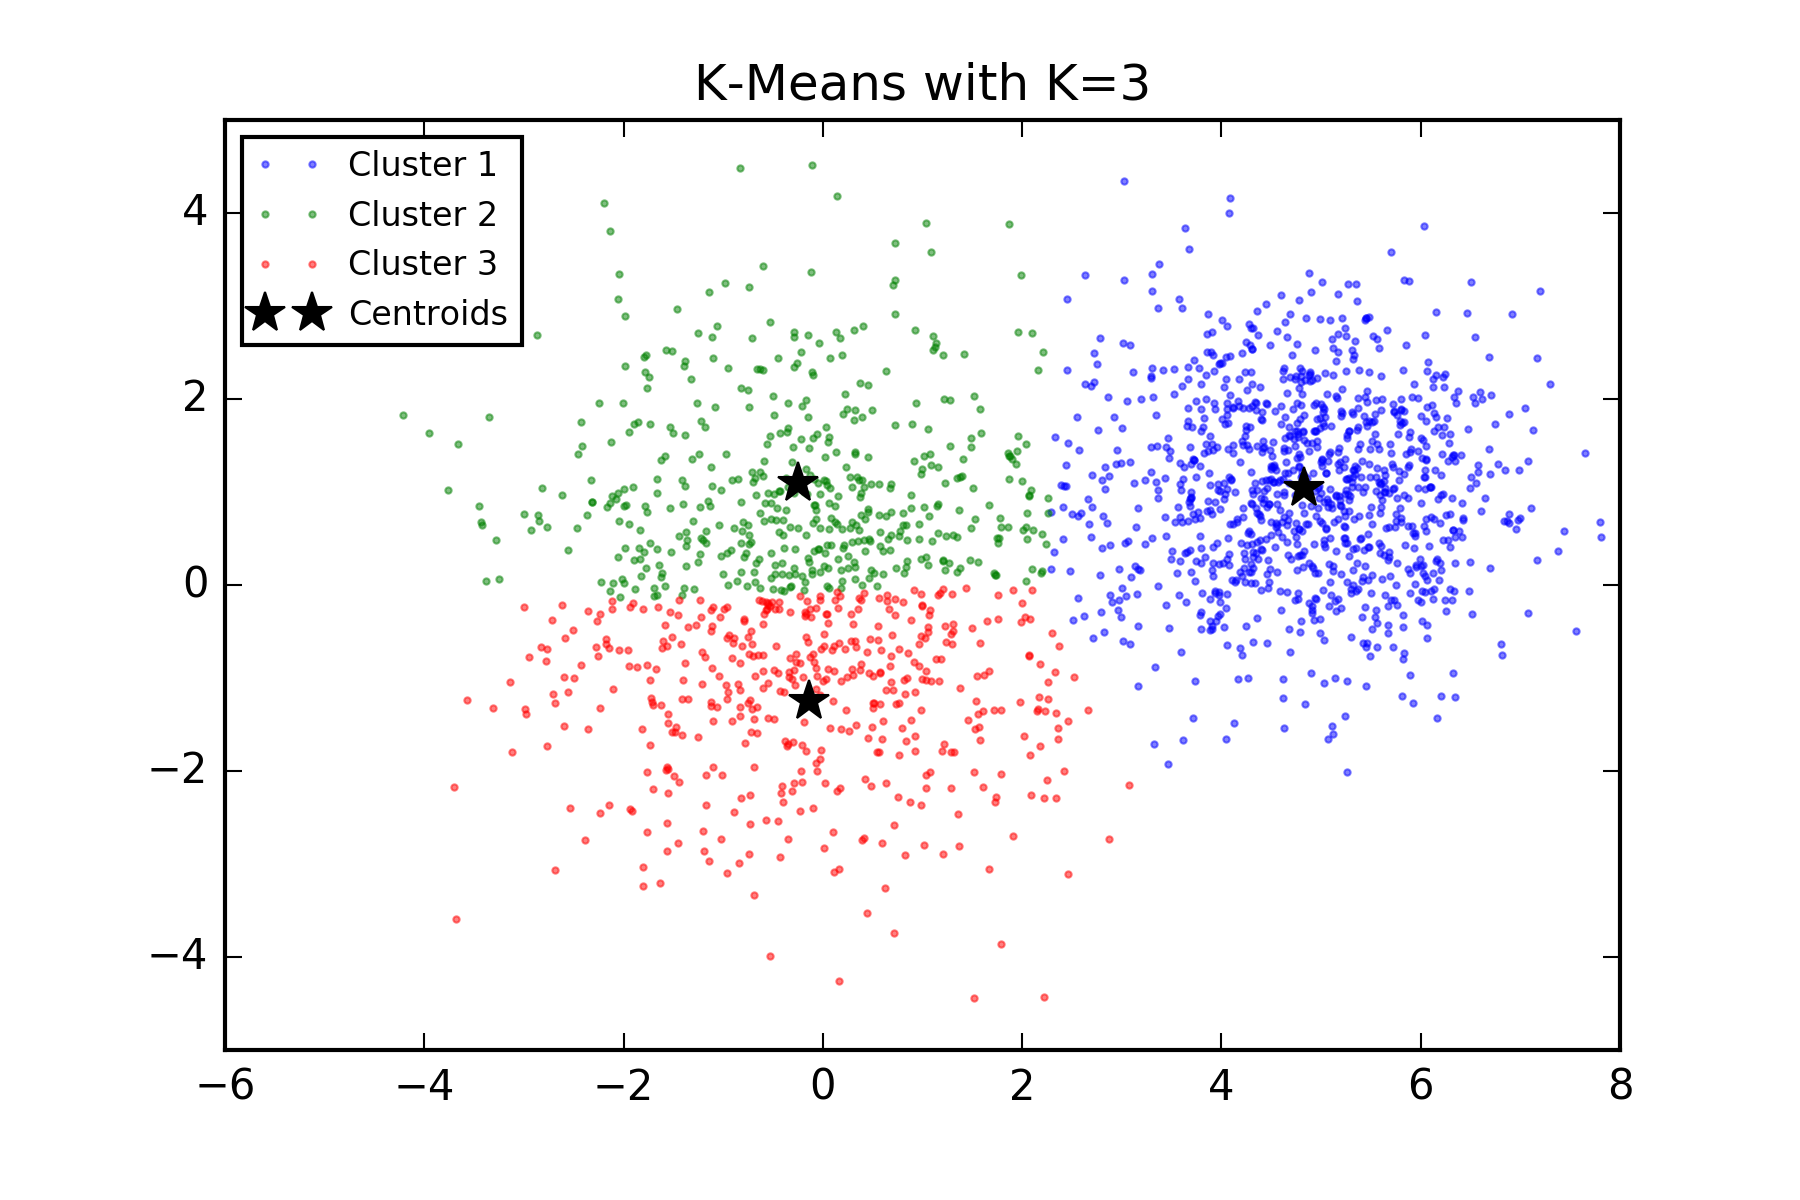
\includegraphics[width=\textwidth]{./figures/clustering_kMeans_3.png}
        \end{subfigure}
        \hfill
        \begin{subfigure}[b]{0.475\textwidth}  
            \centering 
            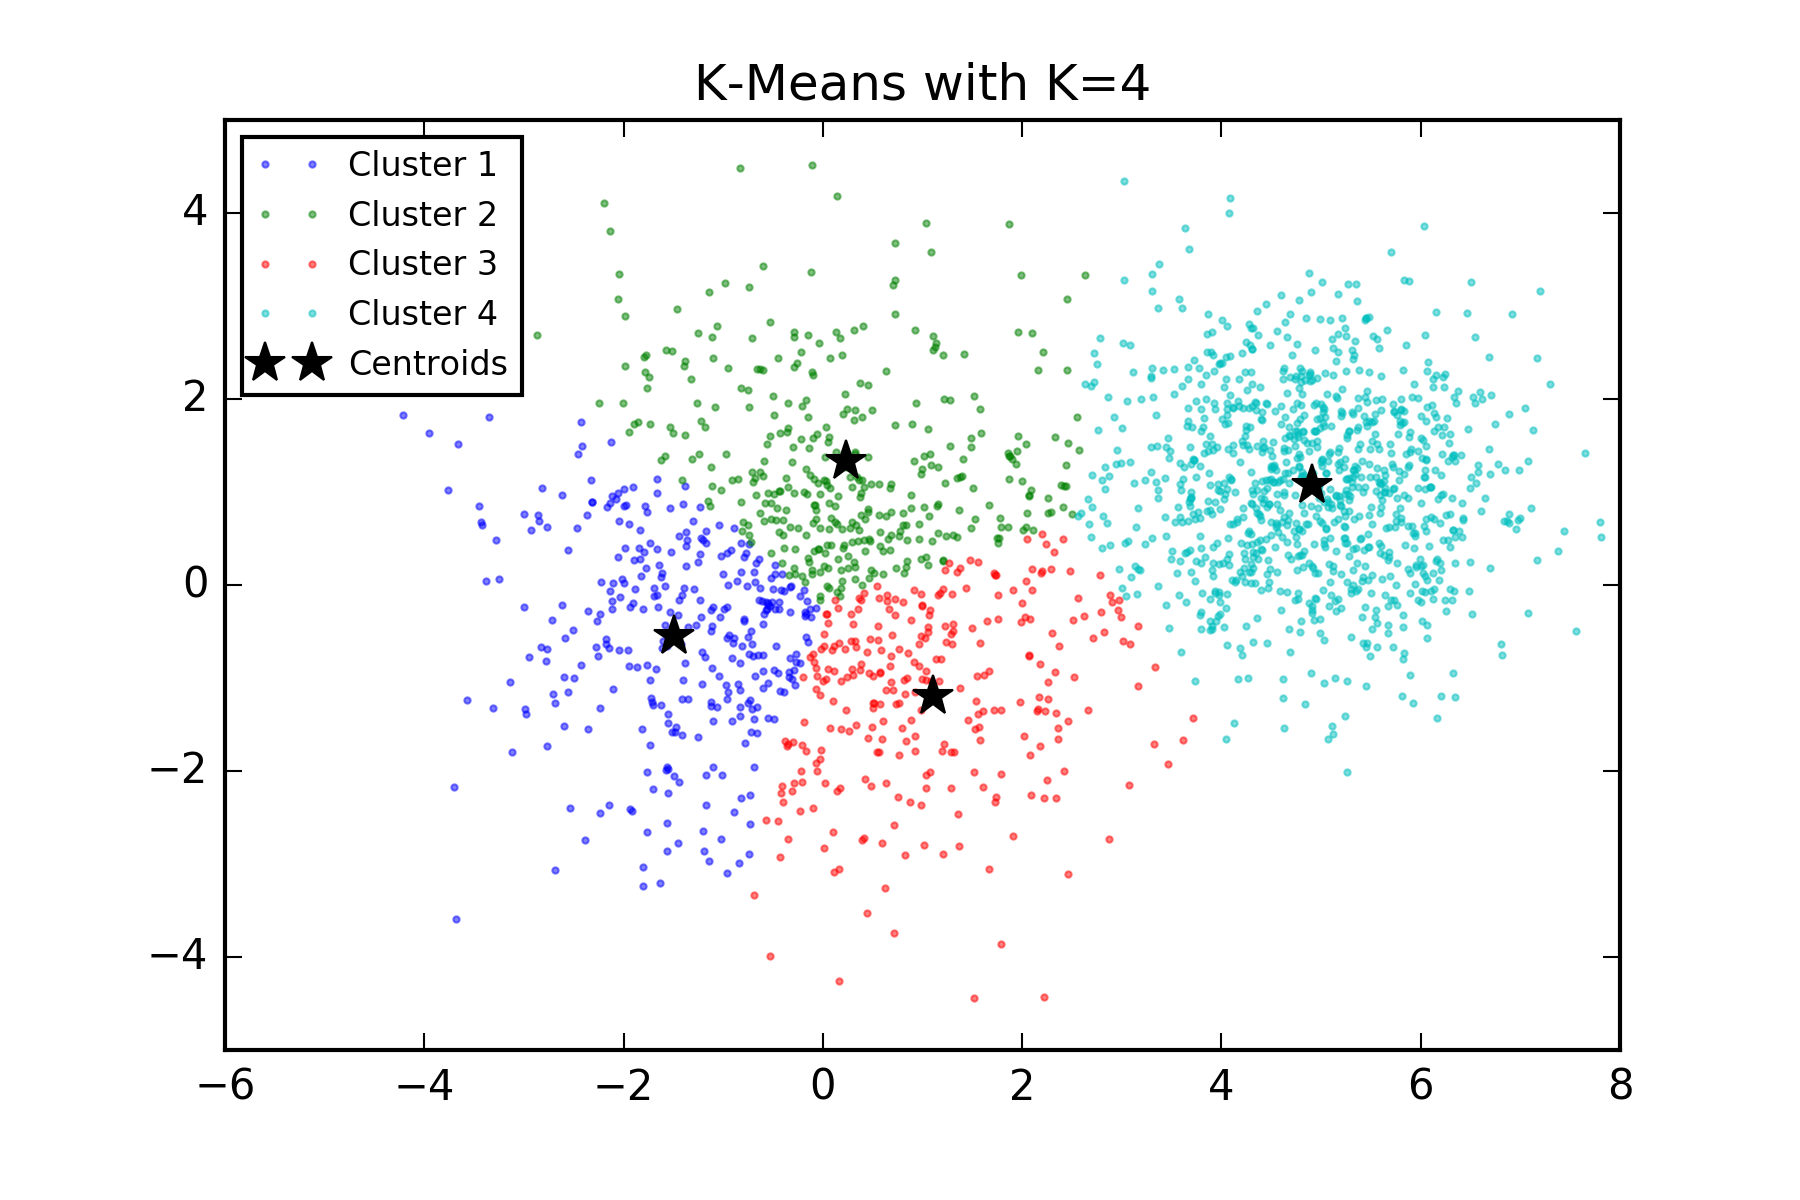
\includegraphics[width=\textwidth]{./figures/clustering_kMeans_4.png}
        \end{subfigure}
%        \vskip\baselineskip        
        \begin{subfigure}[b]{0.475\textwidth}  
            \centering 
            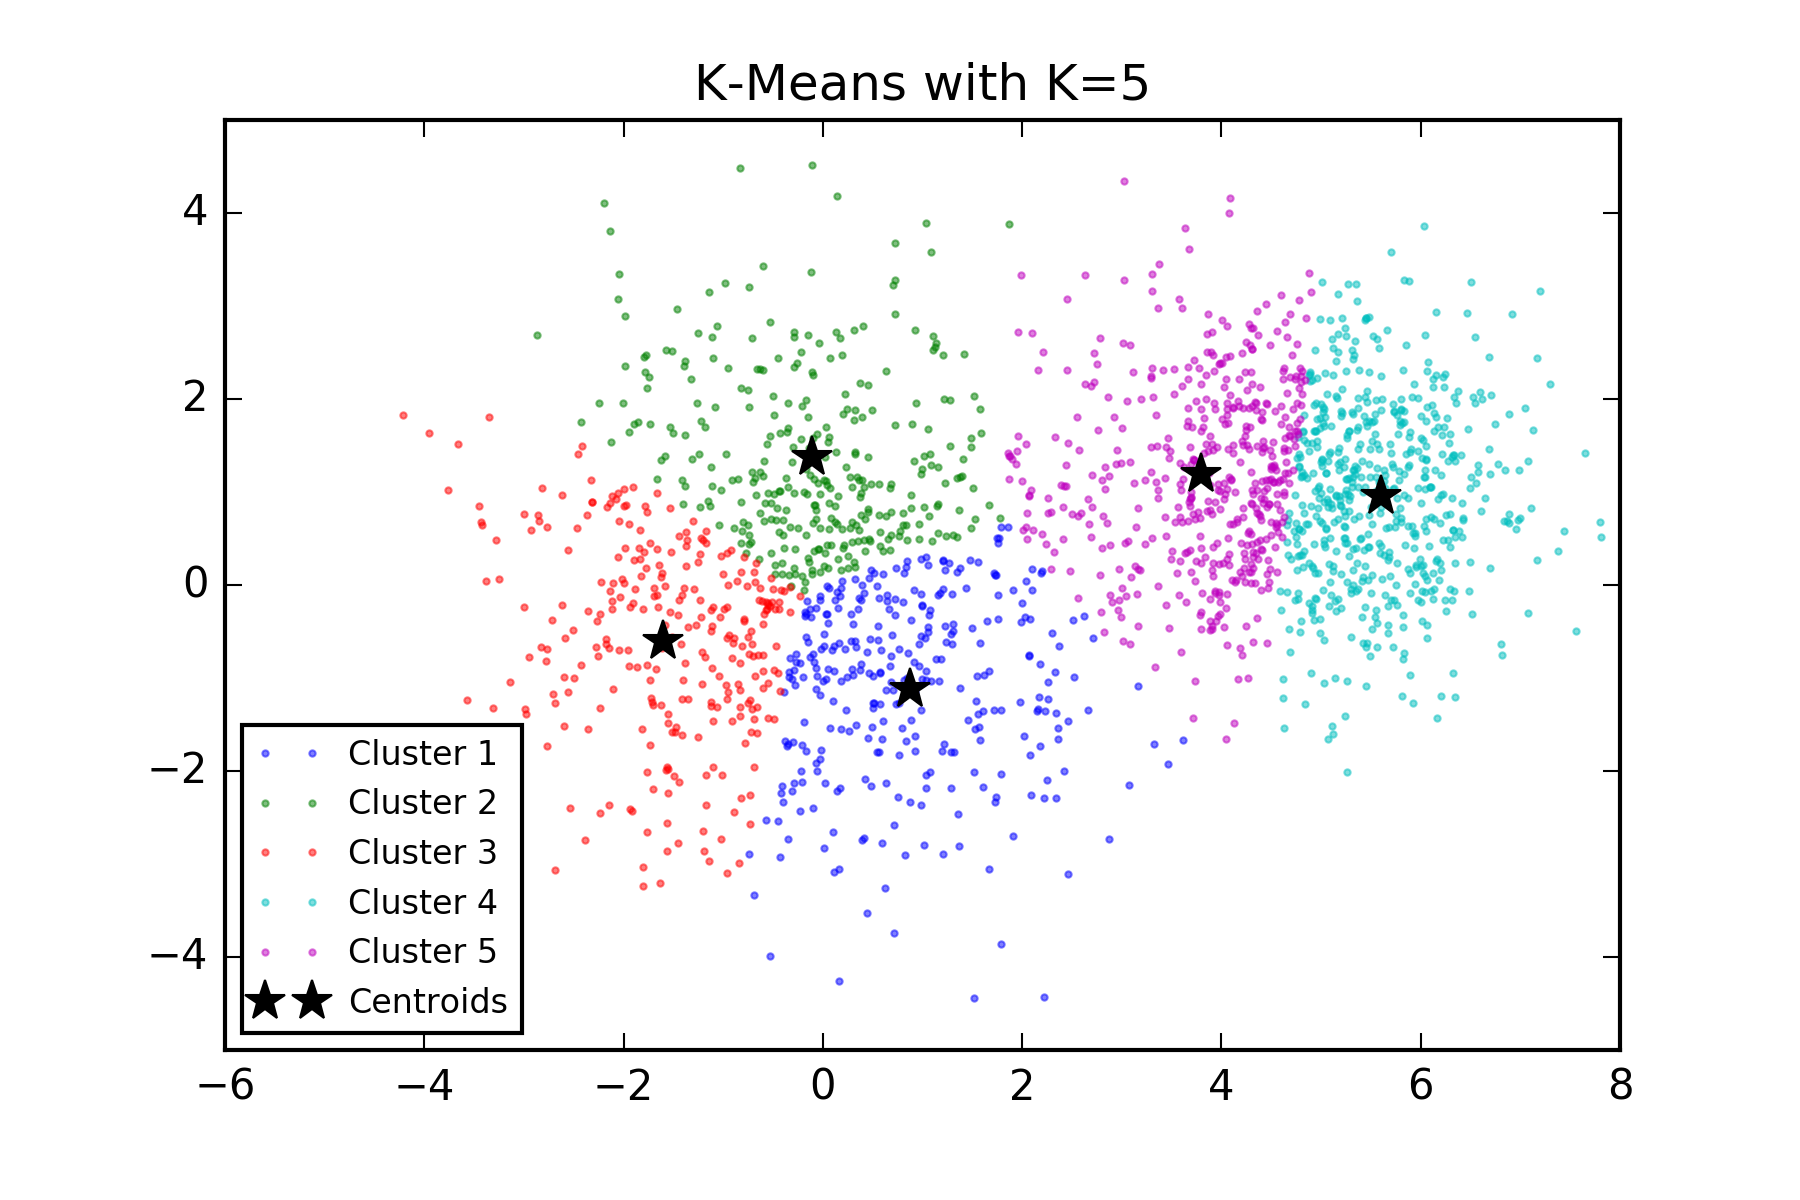
\includegraphics[width=\textwidth]{./figures/clustering_kMeans_5.png}
        \end{subfigure}
        \hfill
        \begin{subfigure}[b]{0.475\textwidth}   
            \centering 
            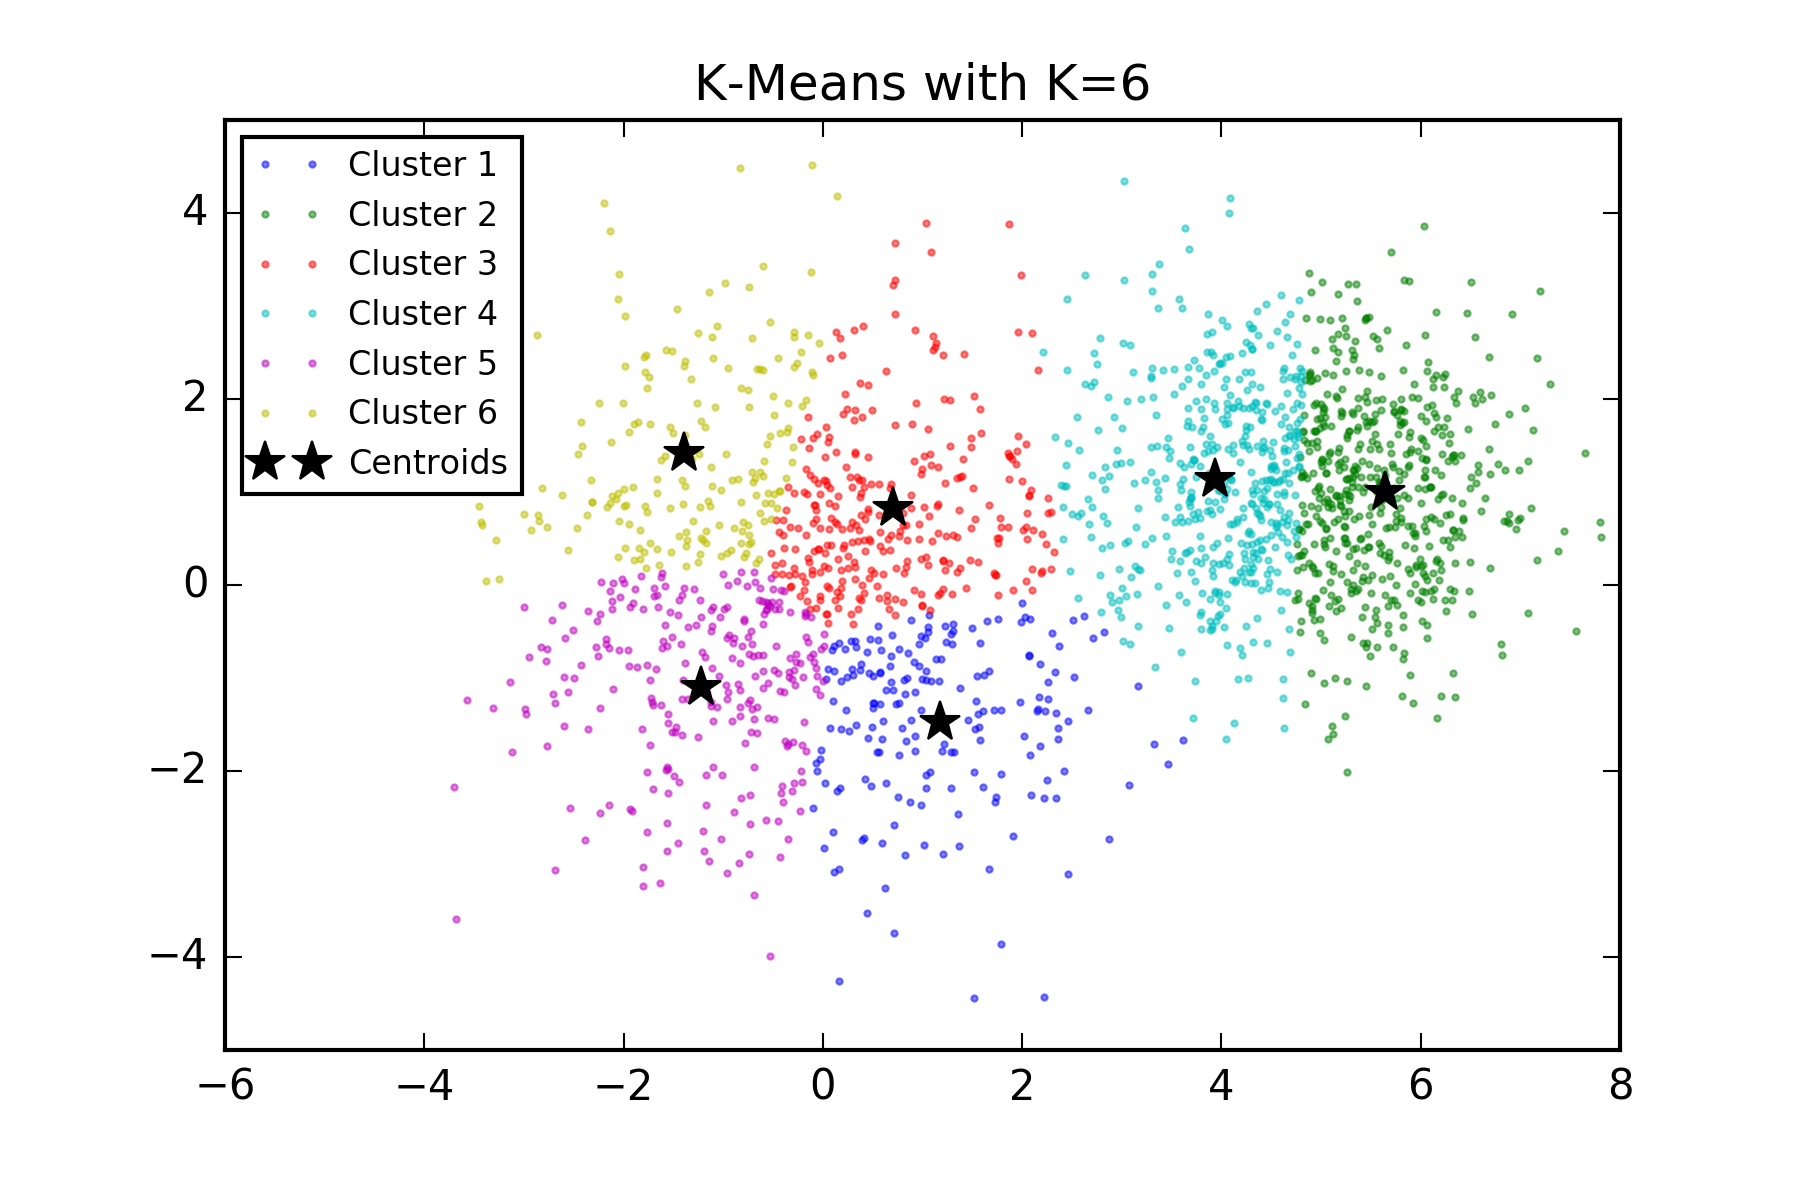
\includegraphics[width=\textwidth]{./figures/clustering_kMeans_6.png}
        \end{subfigure}
%        \vskip\baselineskip     
        \begin{subfigure}[b]{0.475\textwidth}   
            \centering 
            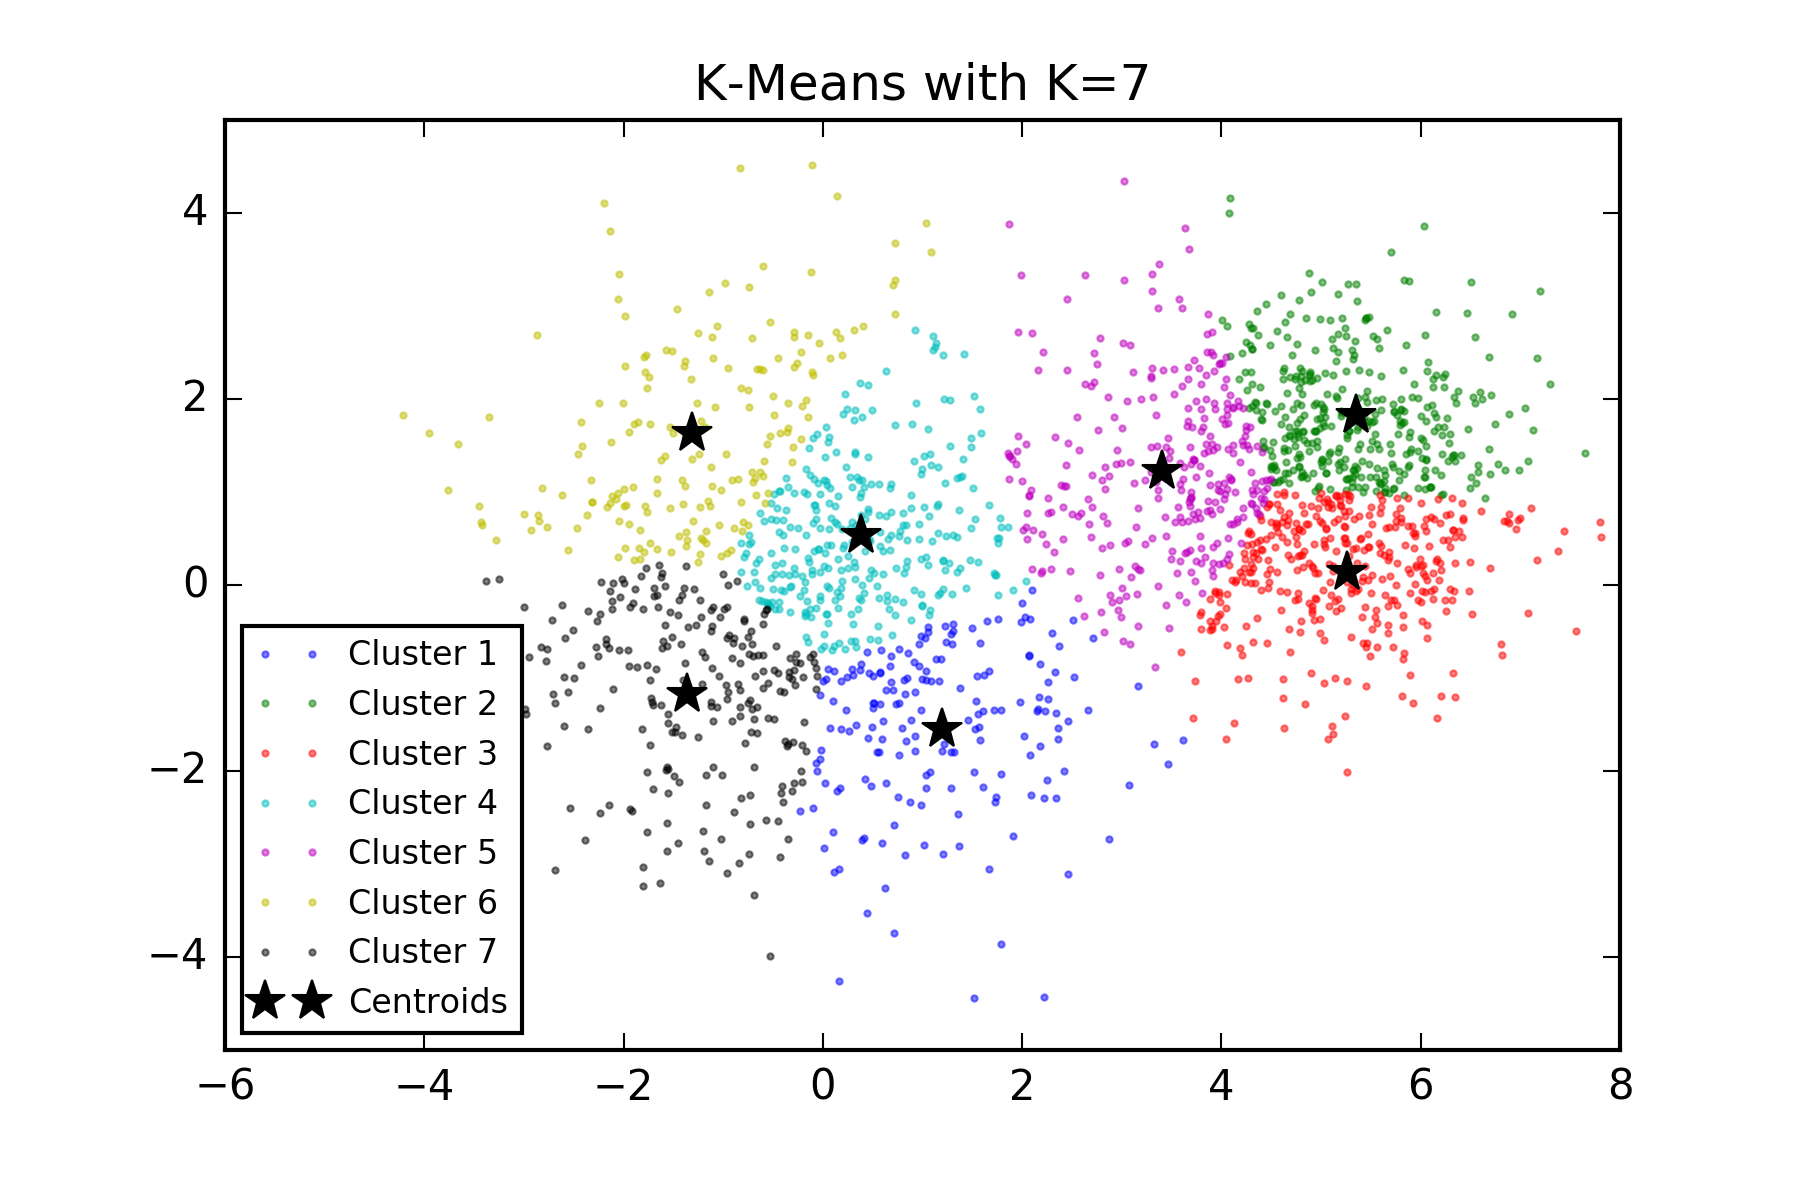
\includegraphics[width=\textwidth]{./figures/clustering_kMeans_7.png}
        \end{subfigure}
        \hfill
        \begin{subfigure}[b]{0.475\textwidth}  
            \centering 
            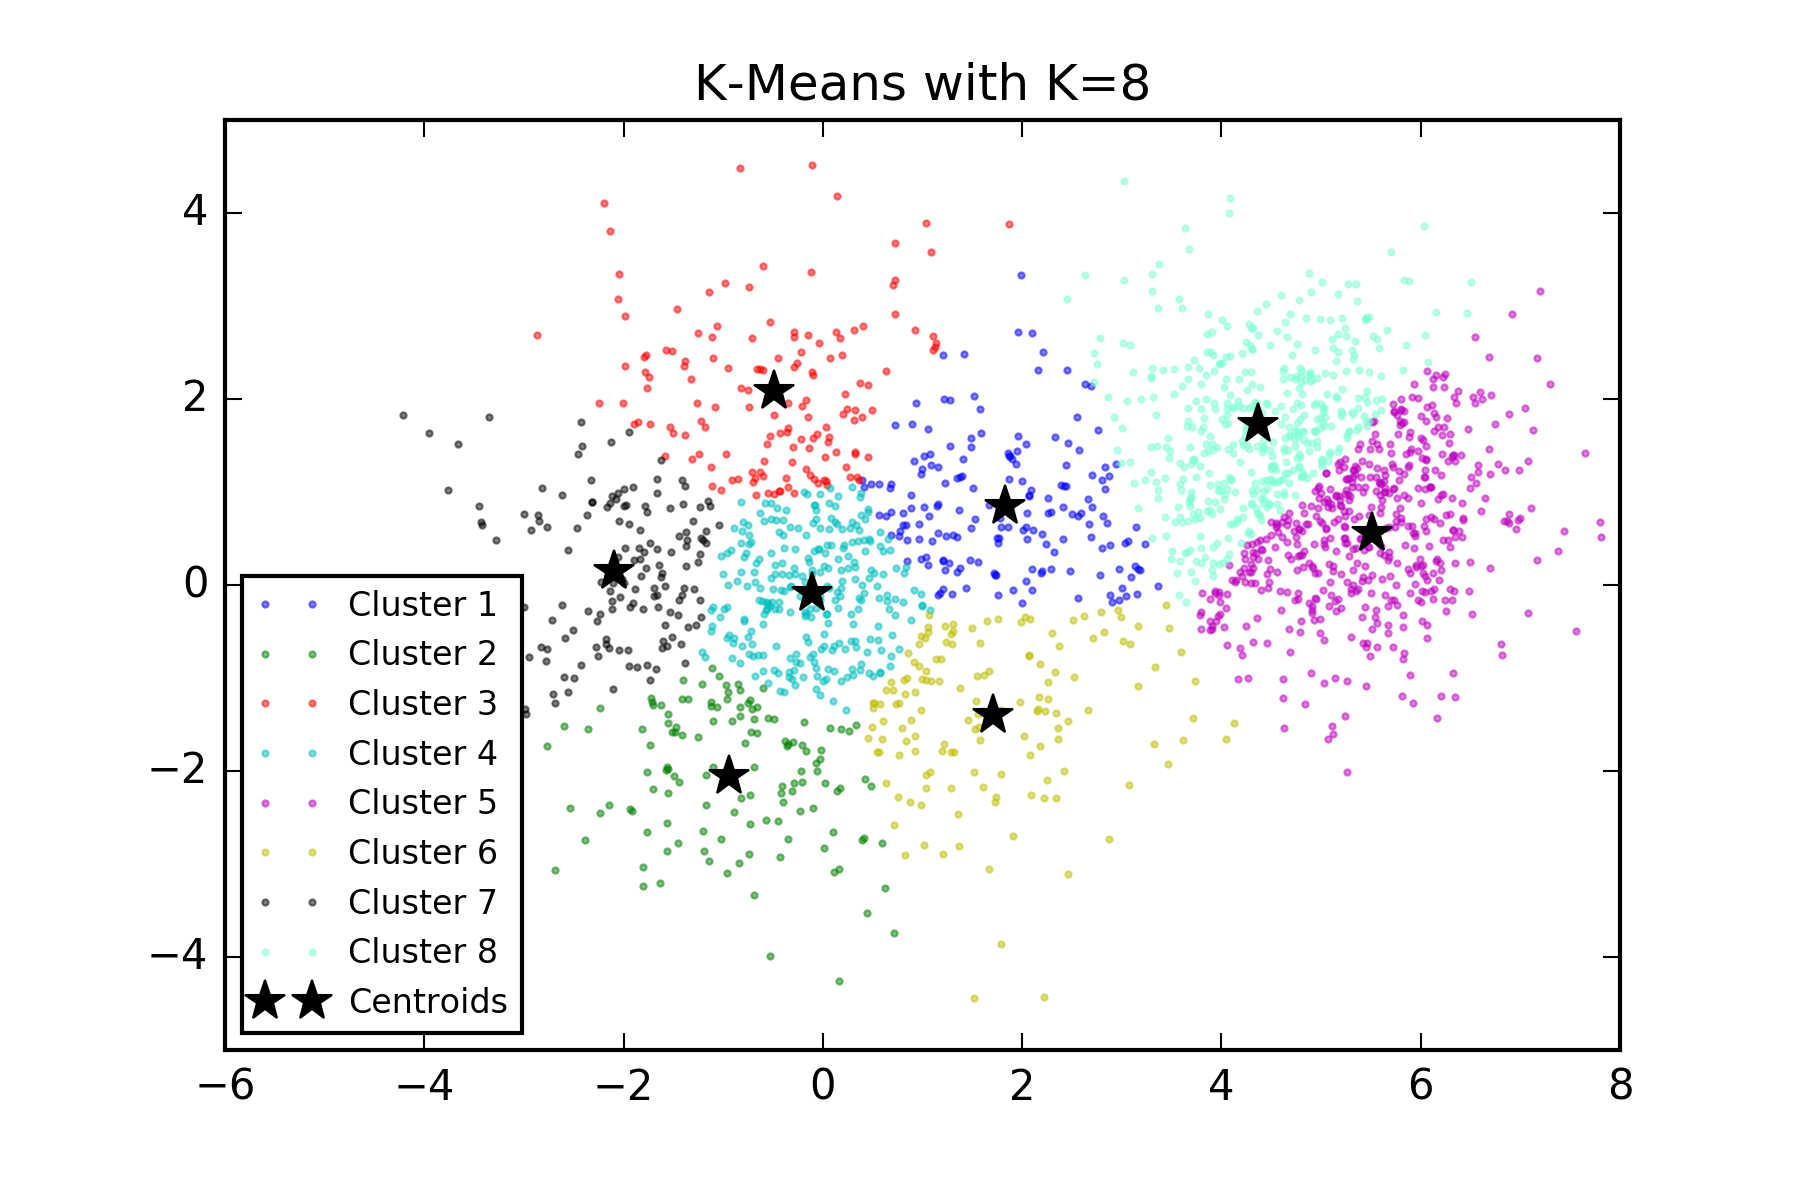
\includegraphics[width=\textwidth]{./figures/clustering_kMeans_8.png}
        \end{subfigure}
%        \vskip\baselineskip
        \begin{subfigure}[b]{0.475\textwidth}   
            \centering 
            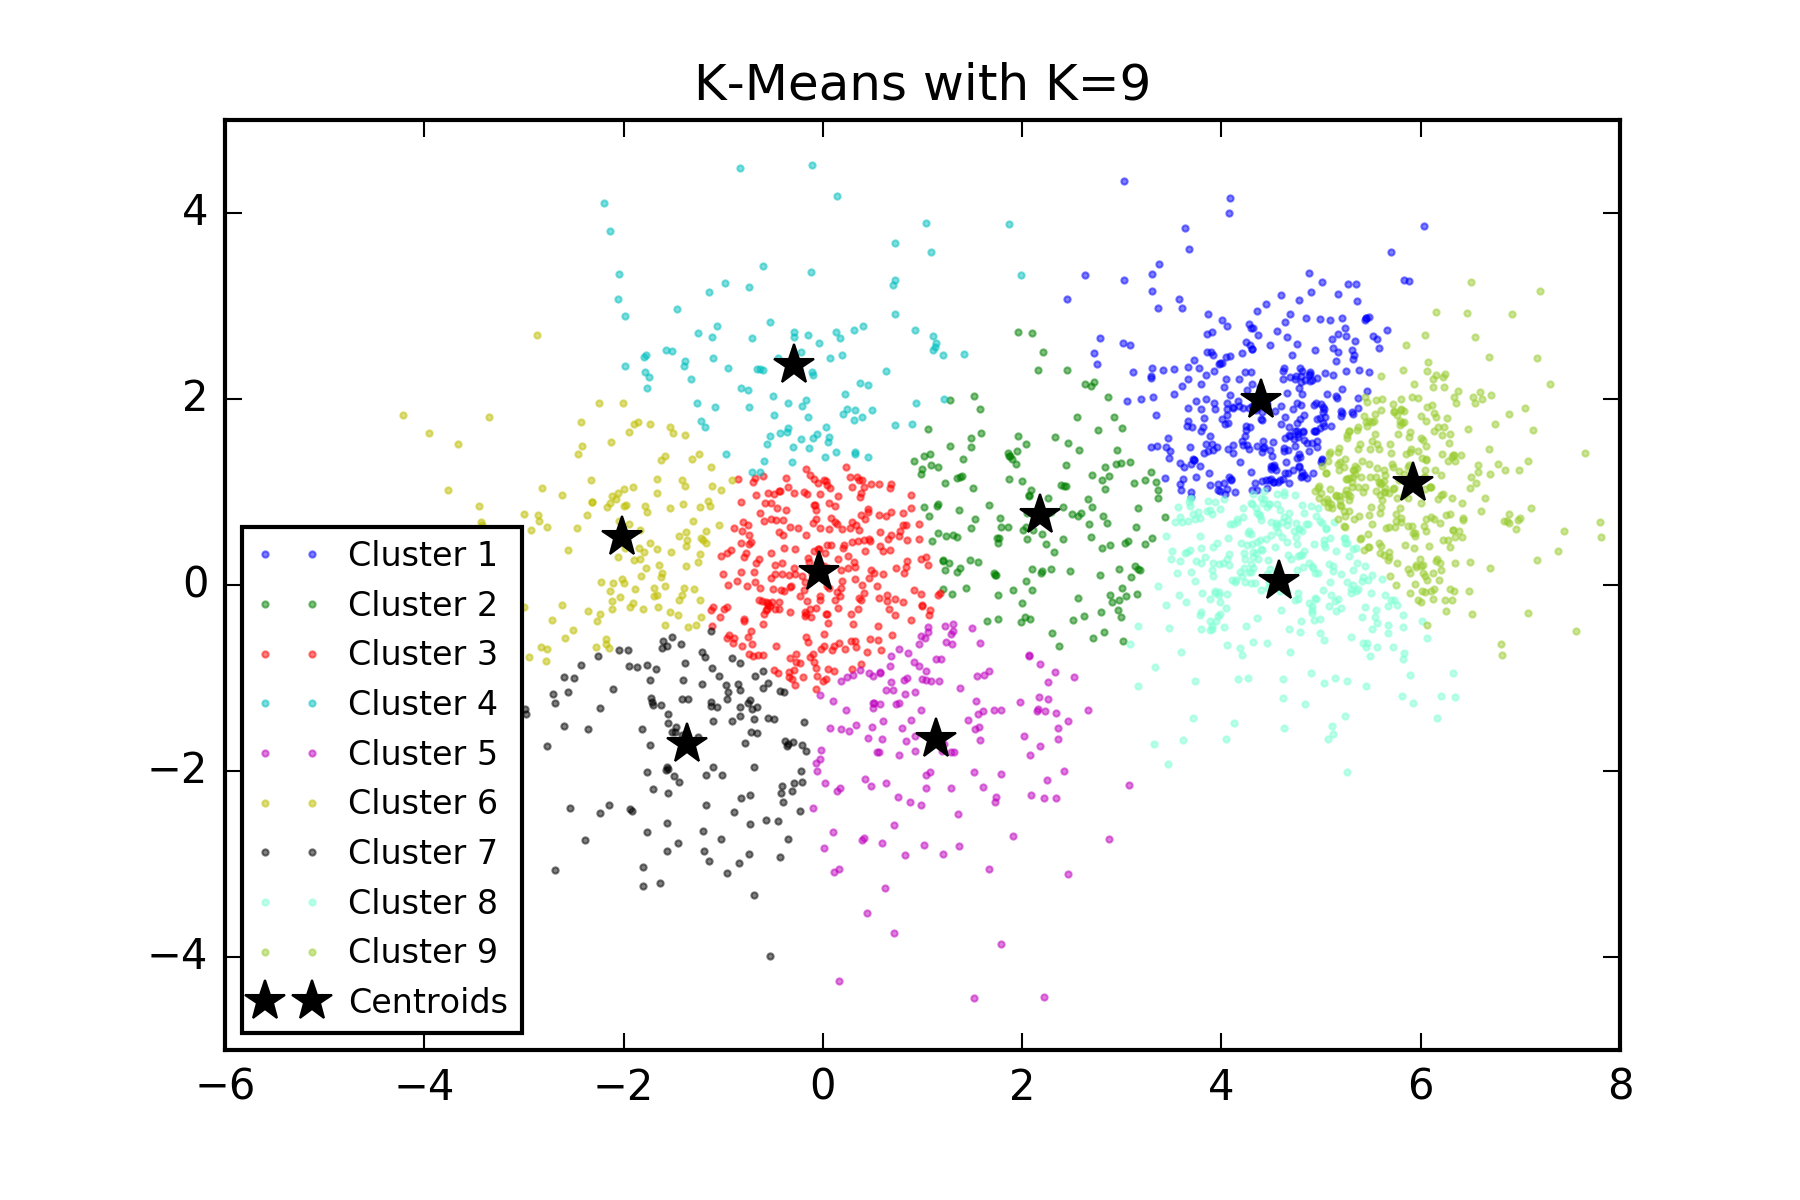
\includegraphics[width=\textwidth]{./figures/clustering_kMeans_9.png}
        \end{subfigure}
        \hfill
        \begin{subfigure}[b]{0.475\textwidth}   
            \centering 
            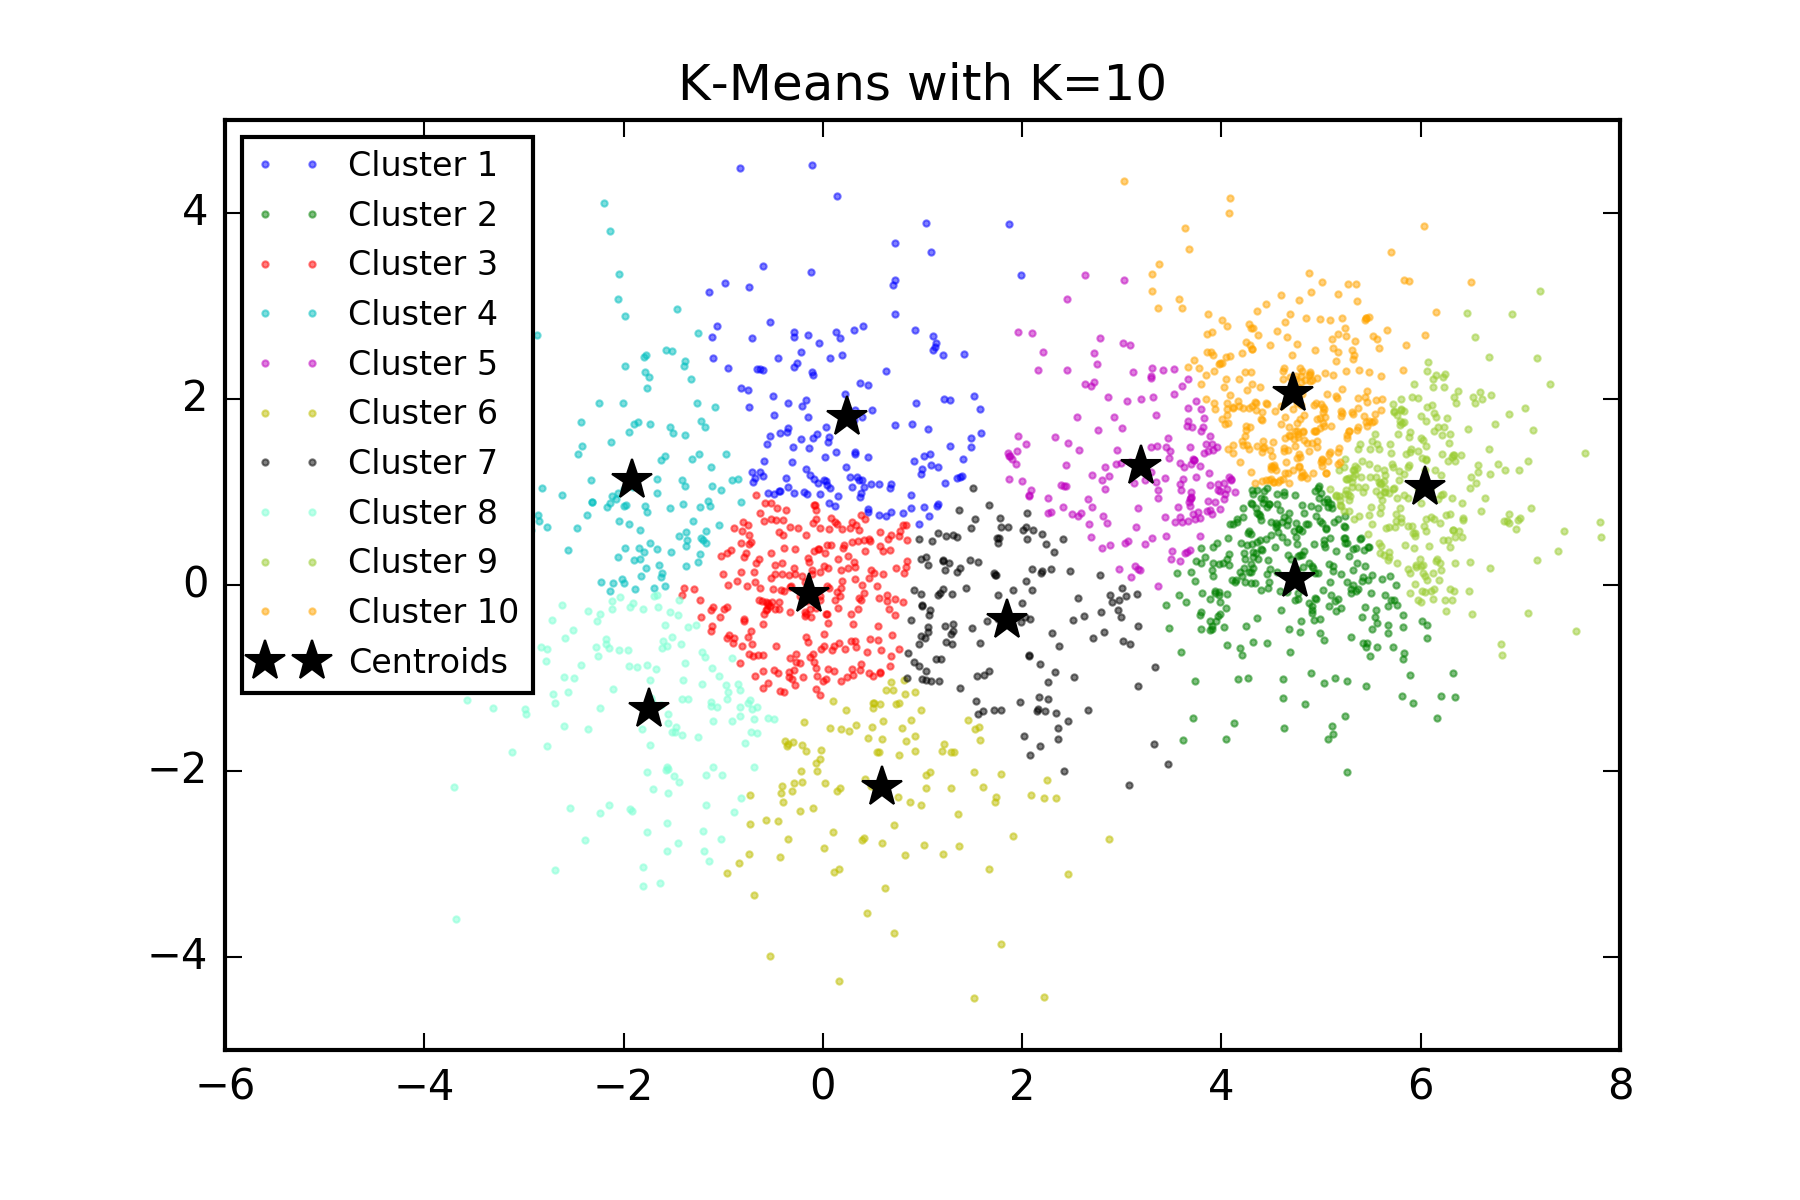
\includegraphics[width=\textwidth]{./figures/clustering_kMeans_10.png}
        \end{subfigure}
        
        \caption{Clustering Result for clustering.txt with K-Means Algorithm}
        \label{fig:kmean_clustering}
\end{figure}

%  -----------------------------------------------------------------------------
\begin{figure}[htb]
        \centering
        \begin{subfigure}[b]{0.475\textwidth}
            \centering
            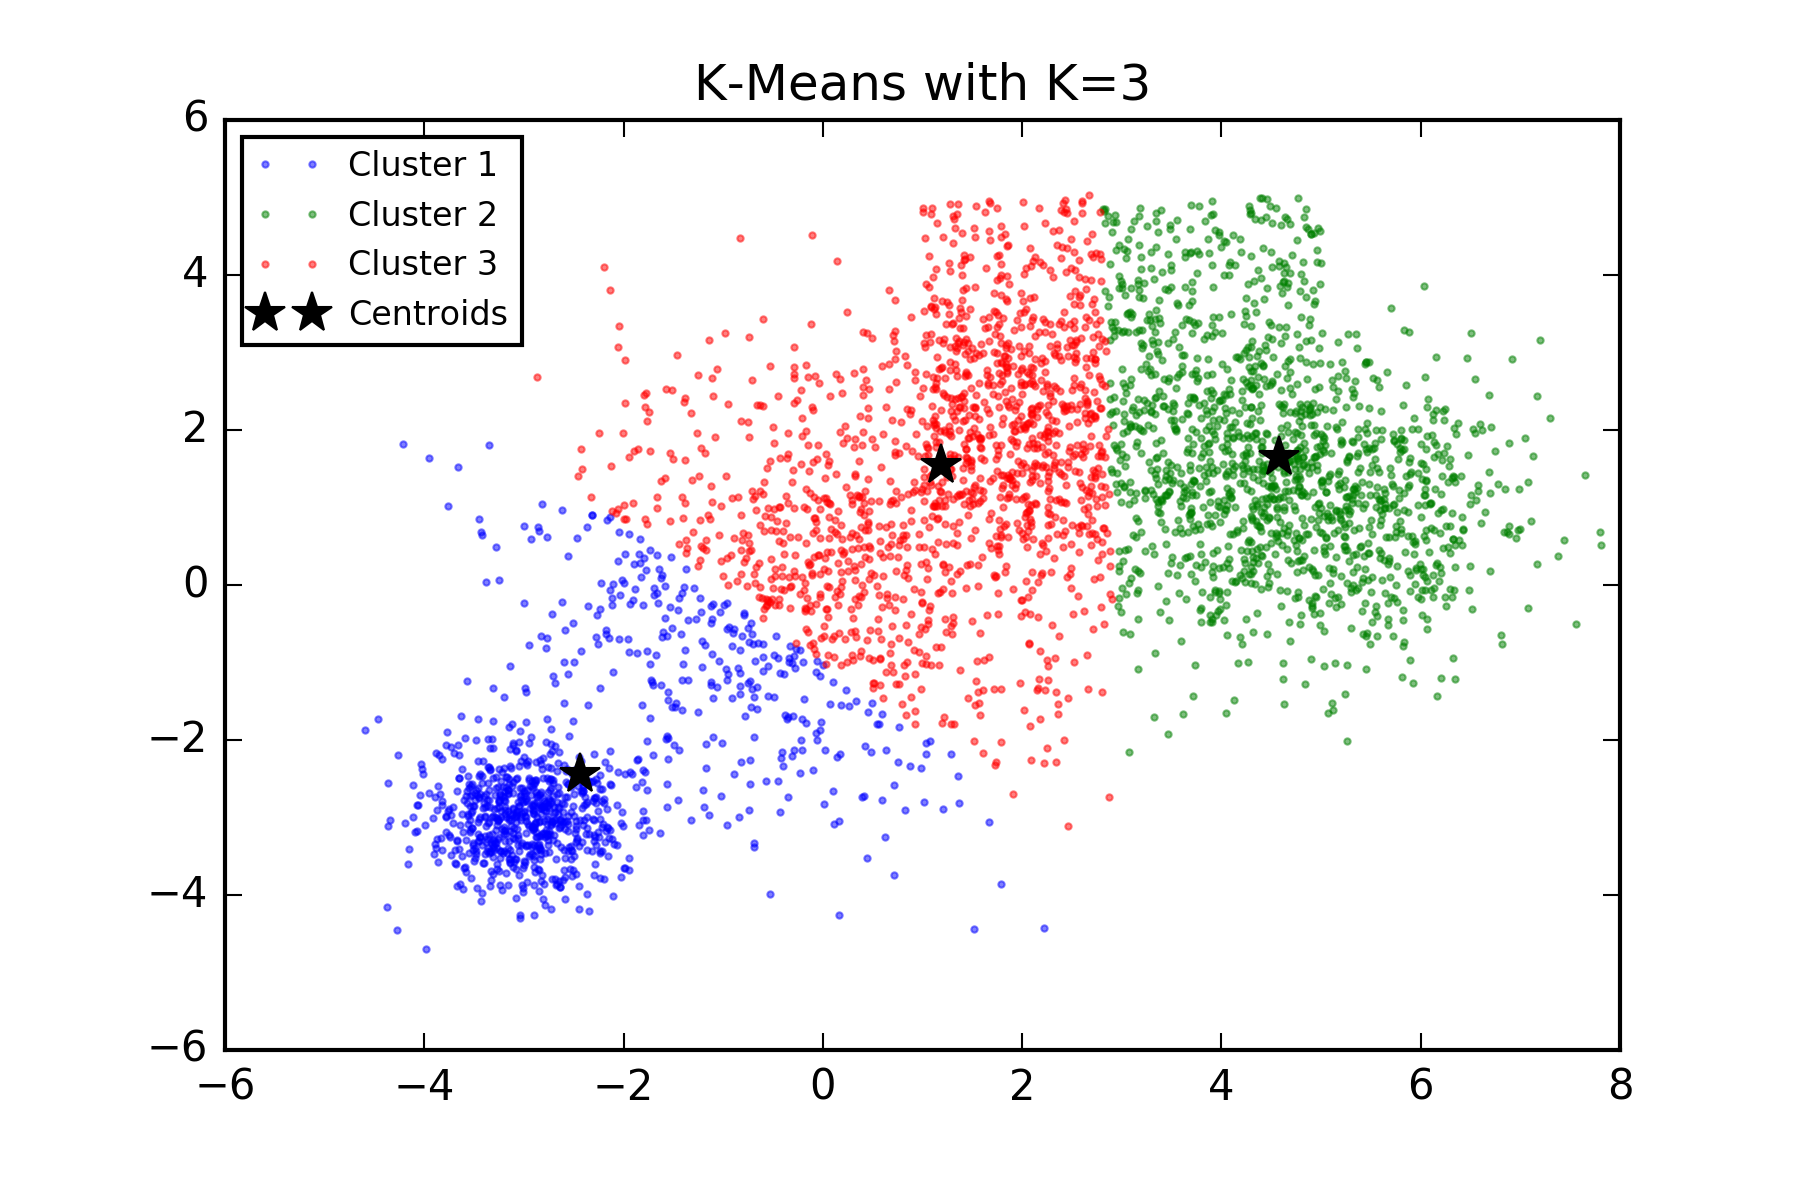
\includegraphics[width=\textwidth]{./figures/bigClustering_kMeans_3.png}
        \end{subfigure}
        \hfill
        \begin{subfigure}[b]{0.475\textwidth}  
            \centering 
            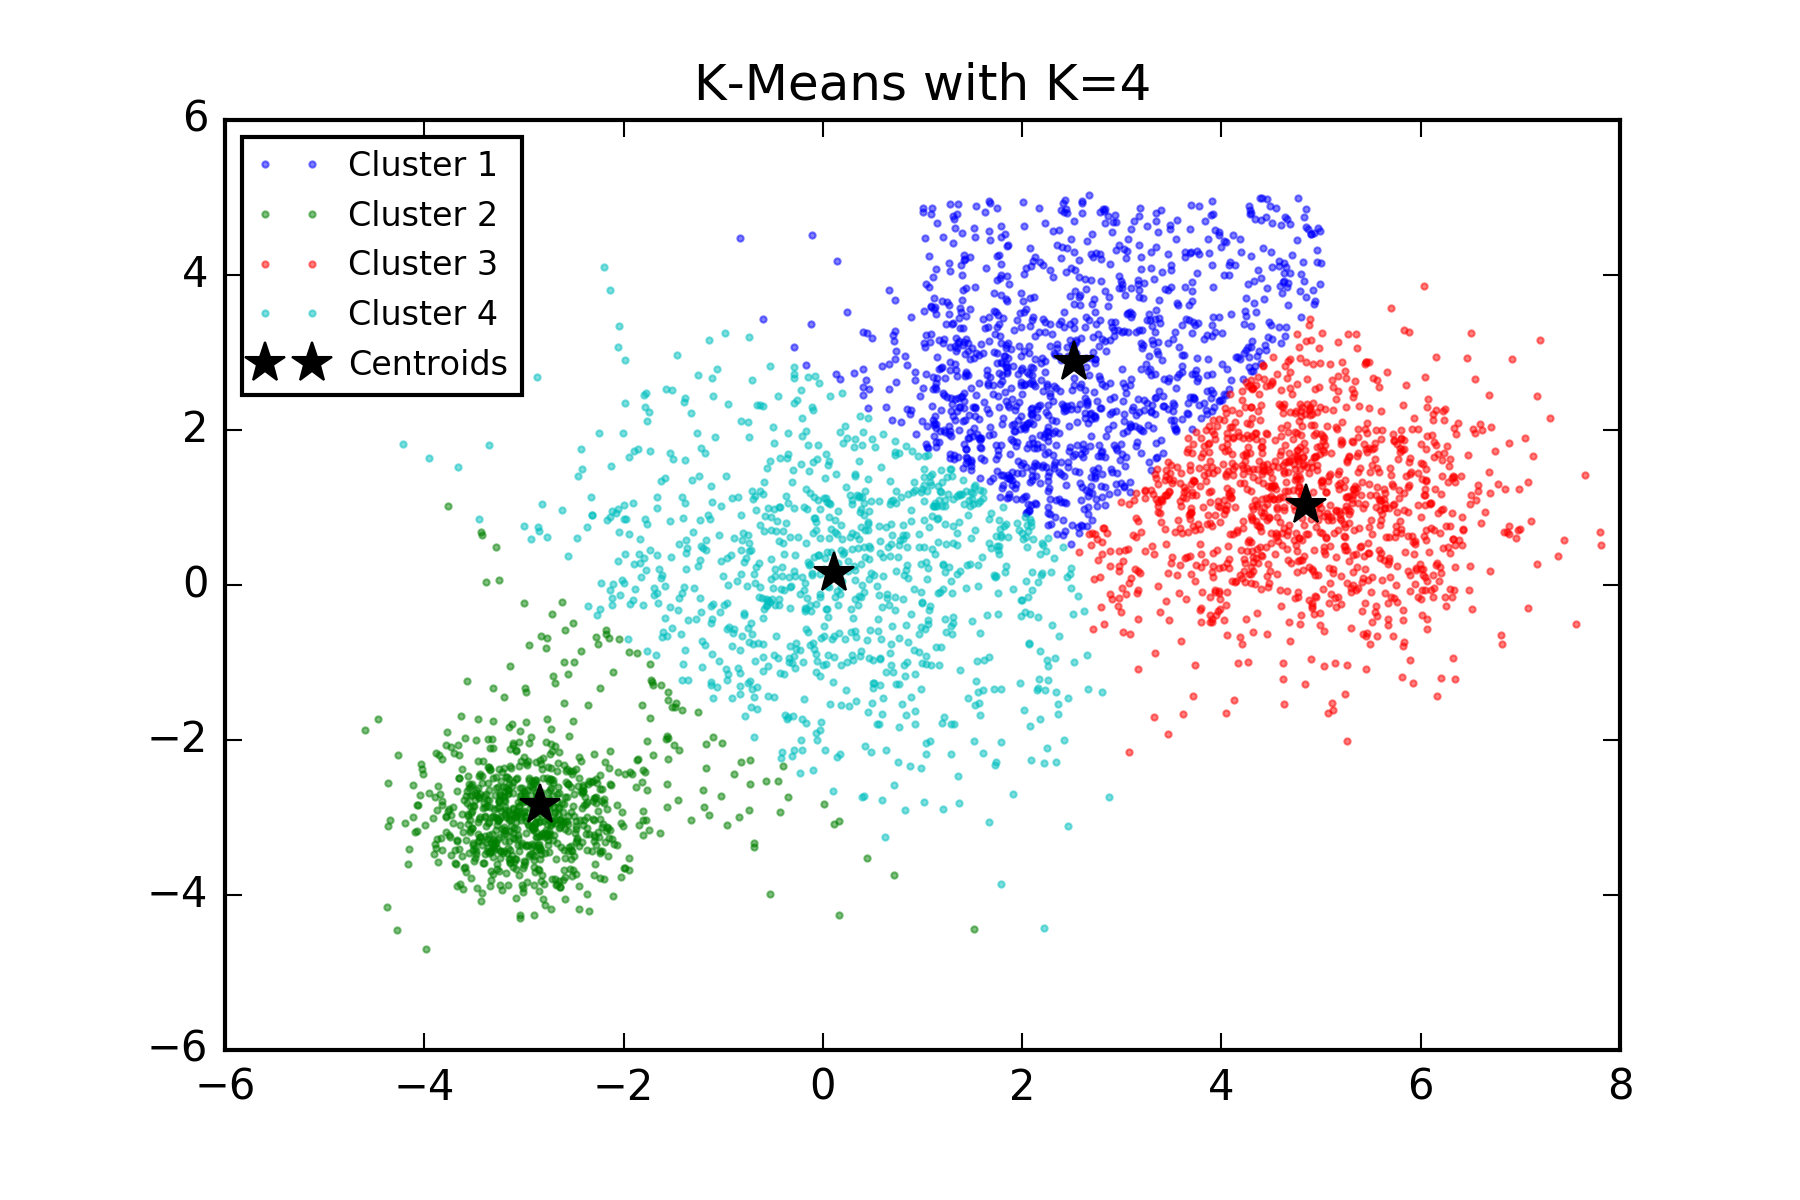
\includegraphics[width=\textwidth]{./figures/bigClustering_kMeans_4.png}
        \end{subfigure}
%        \vskip\baselineskip        
        \begin{subfigure}[b]{0.475\textwidth}  
            \centering 
            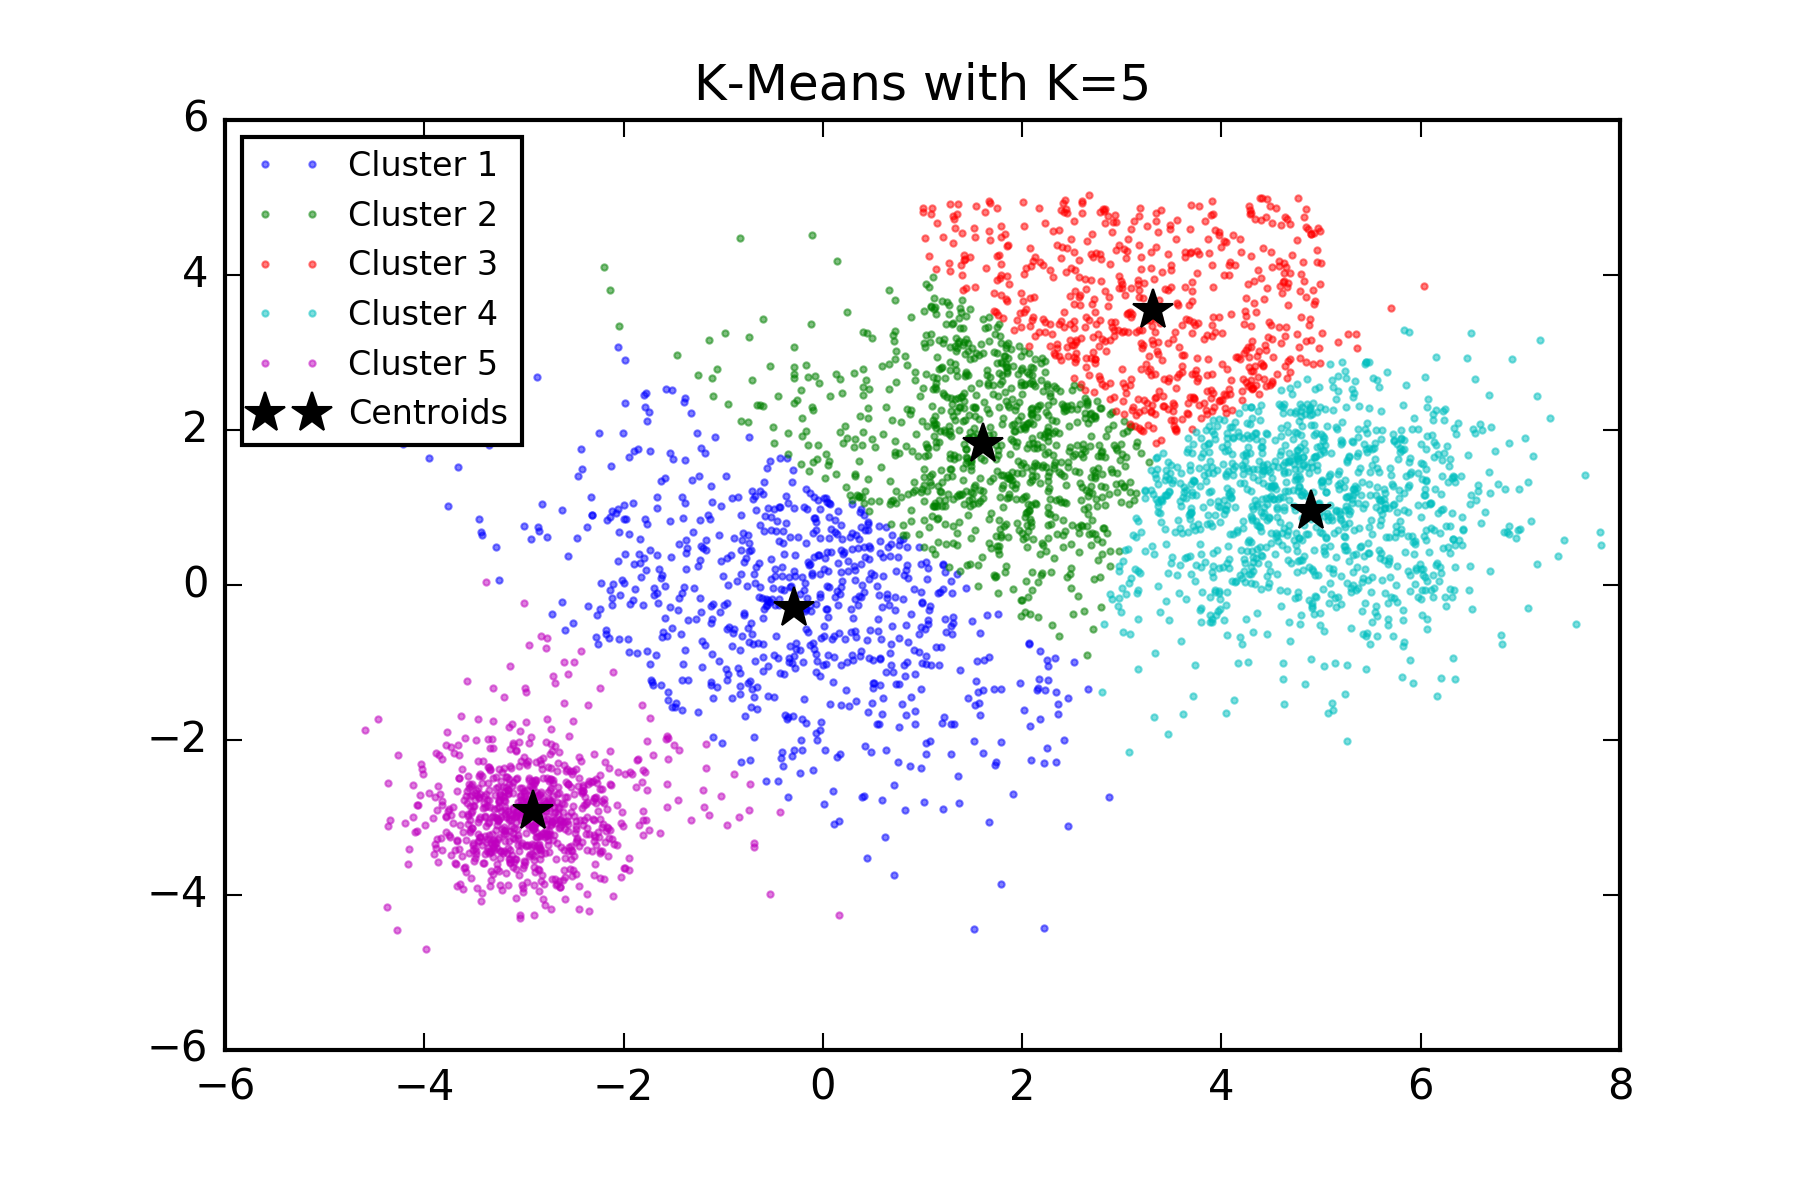
\includegraphics[width=\textwidth]{./figures/bigClustering_kMeans_5.png}
        \end{subfigure}
        \hfill
        \begin{subfigure}[b]{0.475\textwidth}   
            \centering 
            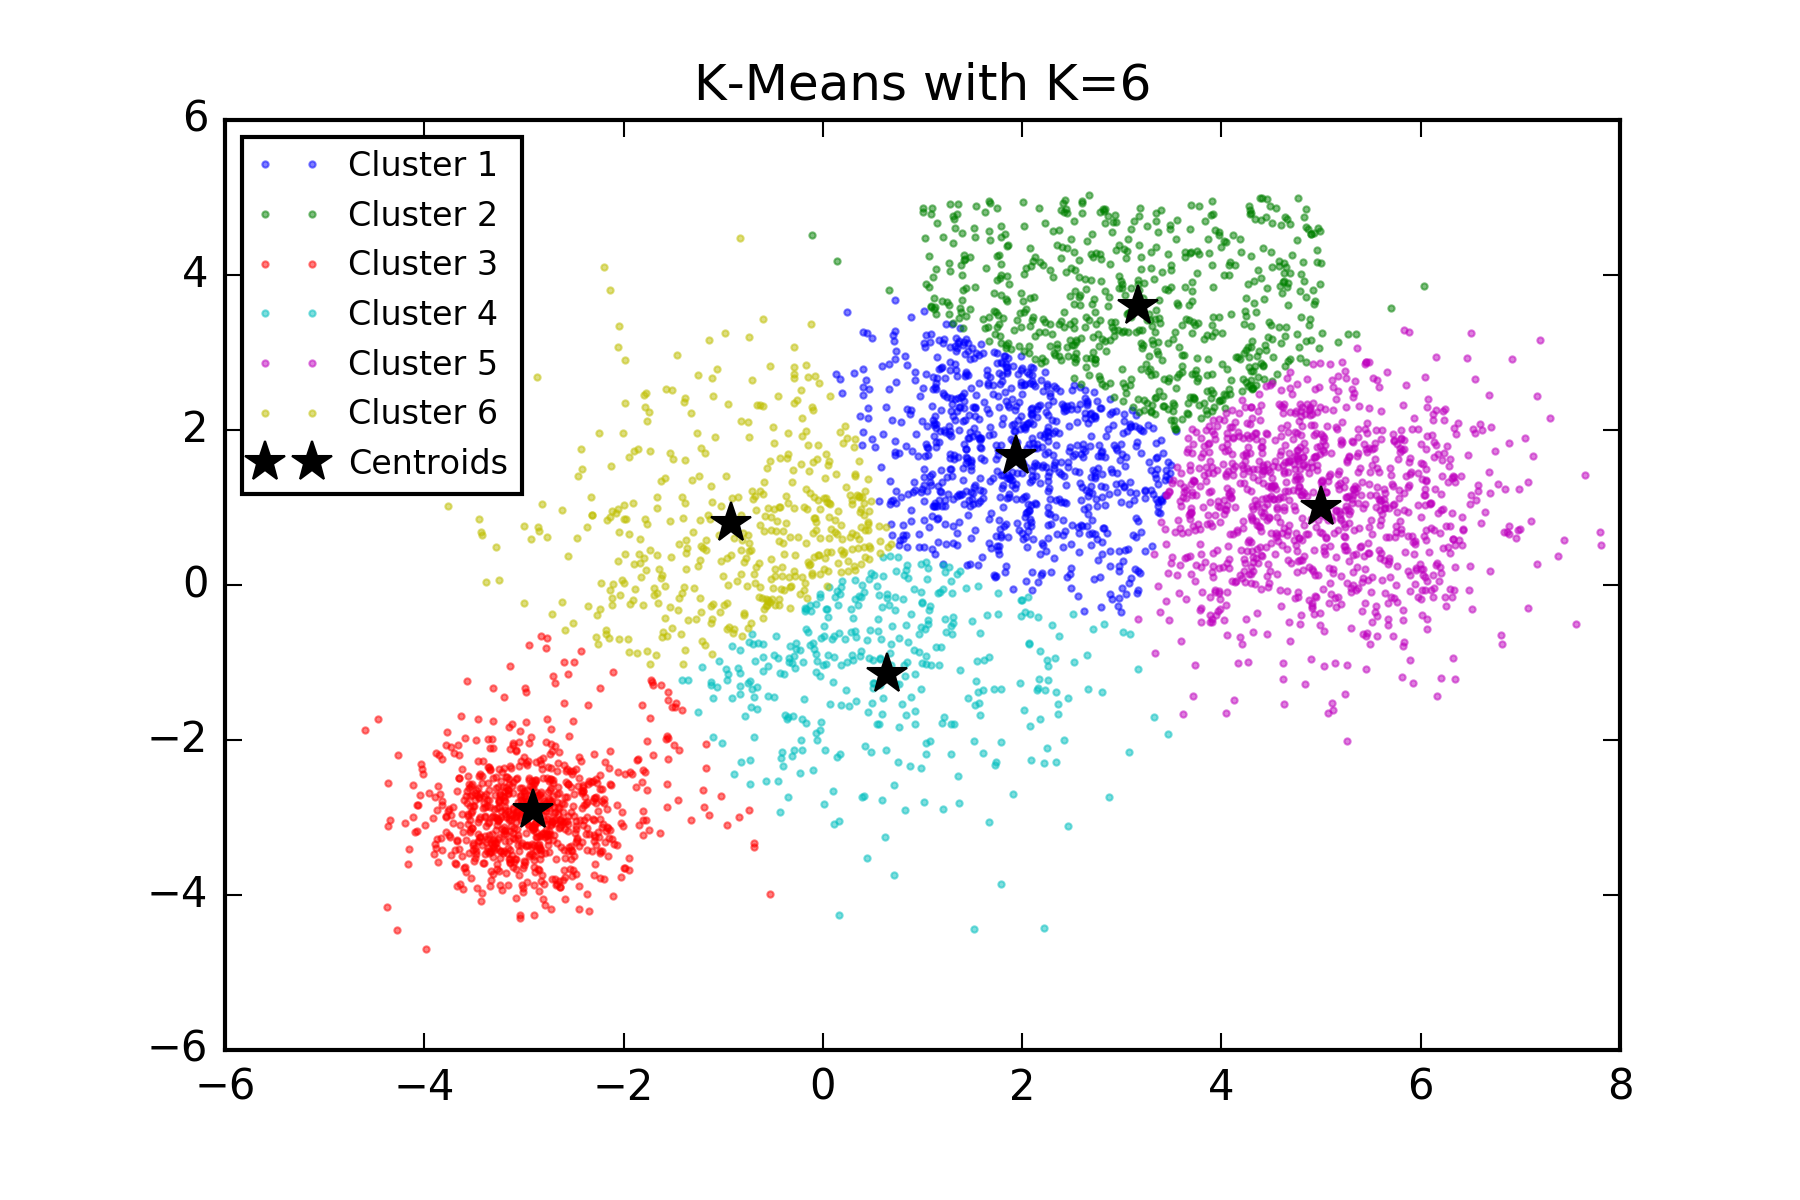
\includegraphics[width=\textwidth]{./figures/bigClustering_kMeans_6.png}
        \end{subfigure}
%        \vskip\baselineskip     
        \begin{subfigure}[b]{0.475\textwidth}   
            \centering 
            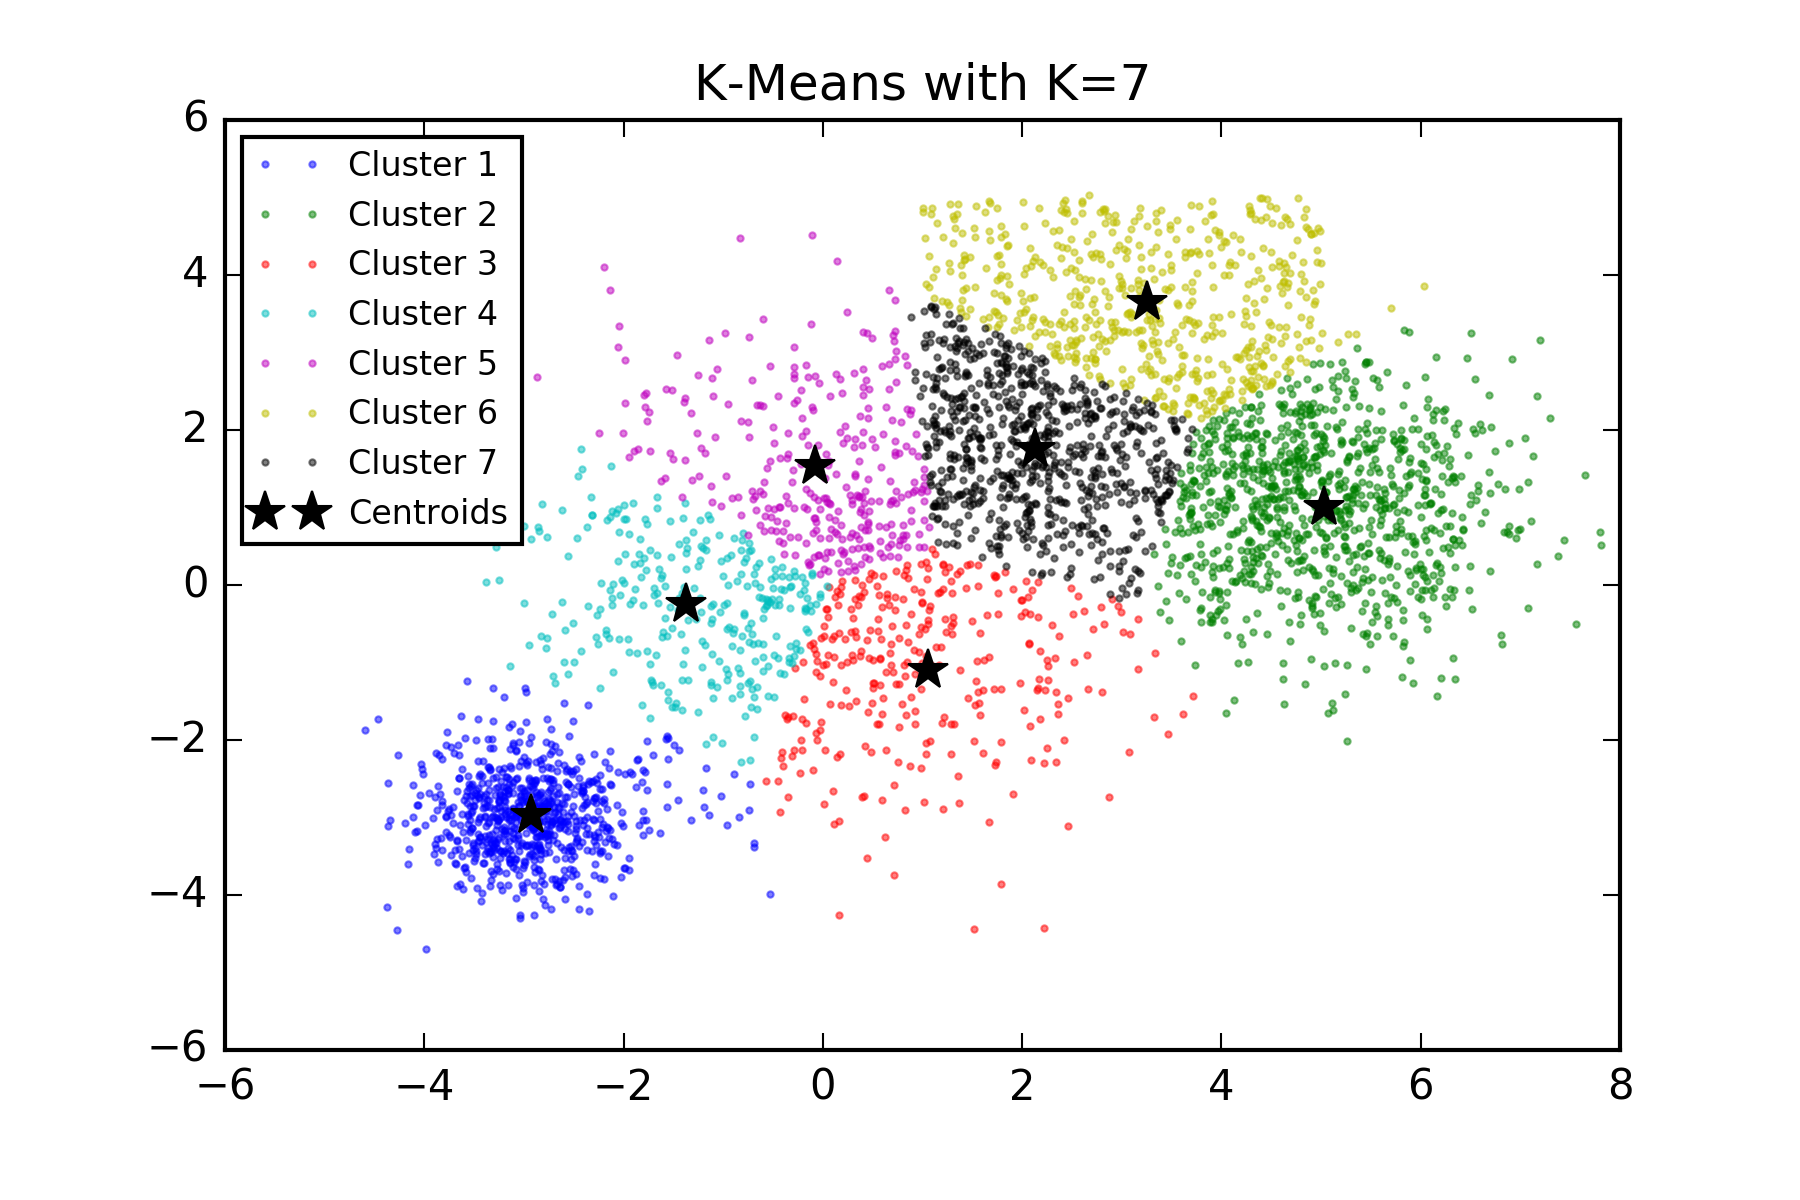
\includegraphics[width=\textwidth]{./figures/bigClustering_kMeans_7.png}
        \end{subfigure}
        \hfill
        \begin{subfigure}[b]{0.475\textwidth}  
            \centering 
            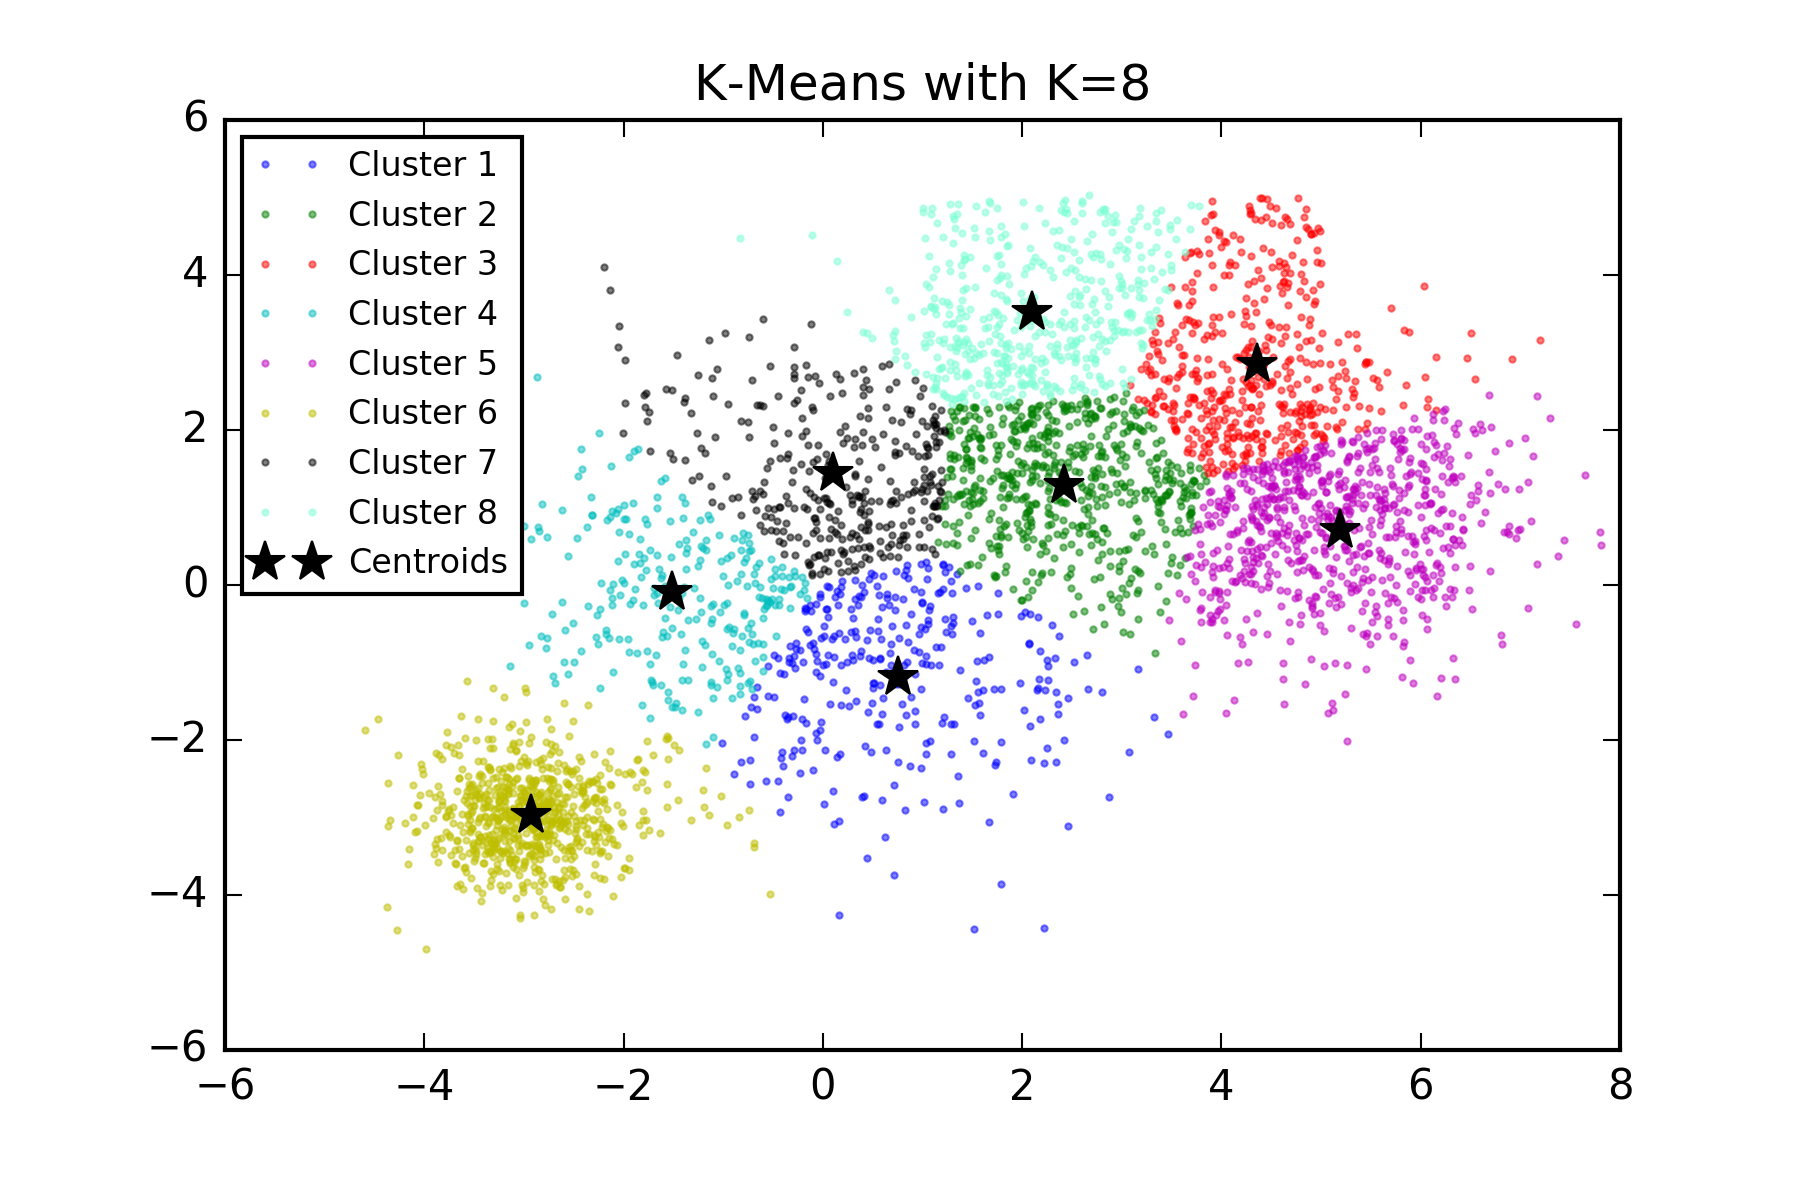
\includegraphics[width=\textwidth]{./figures/bigClustering_kMeans_8.png}
        \end{subfigure}
%        \vskip\baselineskip
        \begin{subfigure}[b]{0.475\textwidth}   
            \centering 
            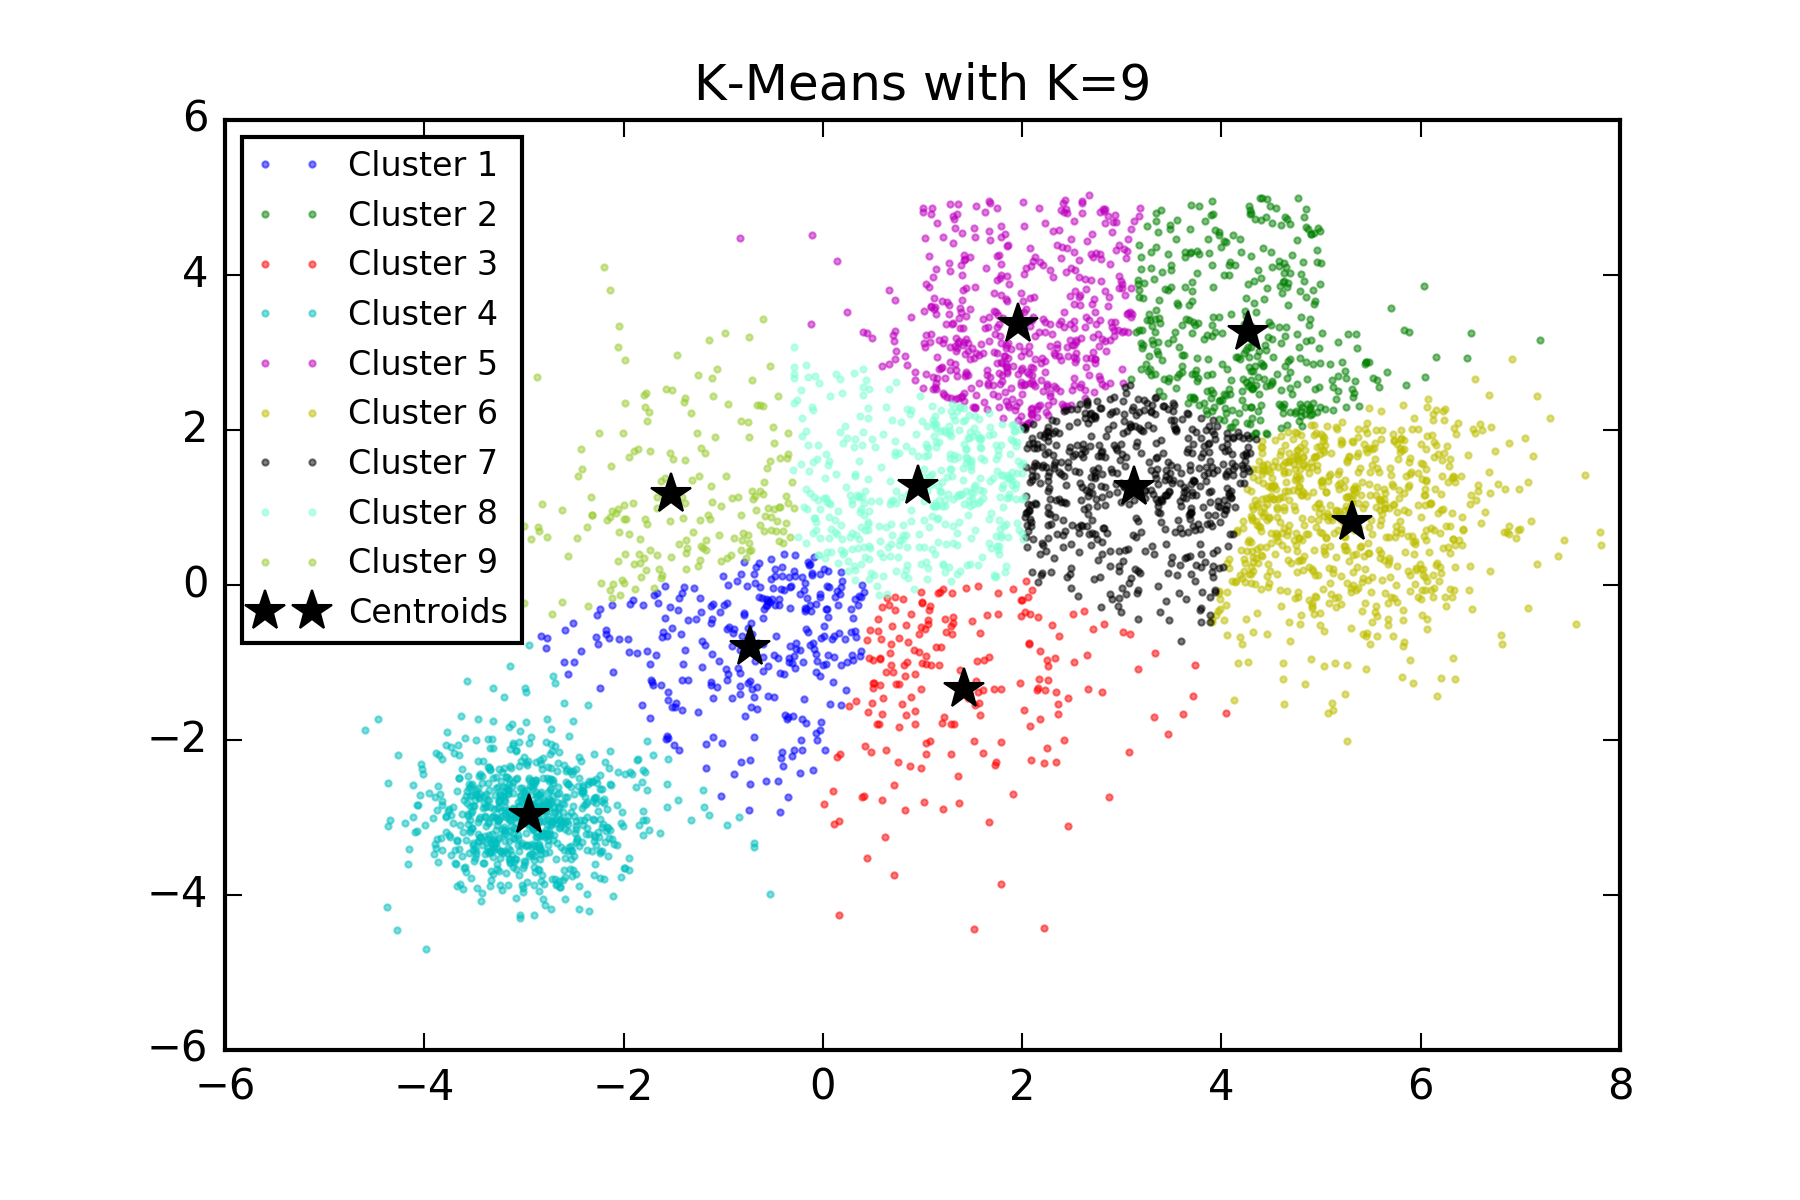
\includegraphics[width=\textwidth]{./figures/bigClustering_kMeans_9.png}
        \end{subfigure}
        \hfill
        \begin{subfigure}[b]{0.475\textwidth}   
            \centering 
            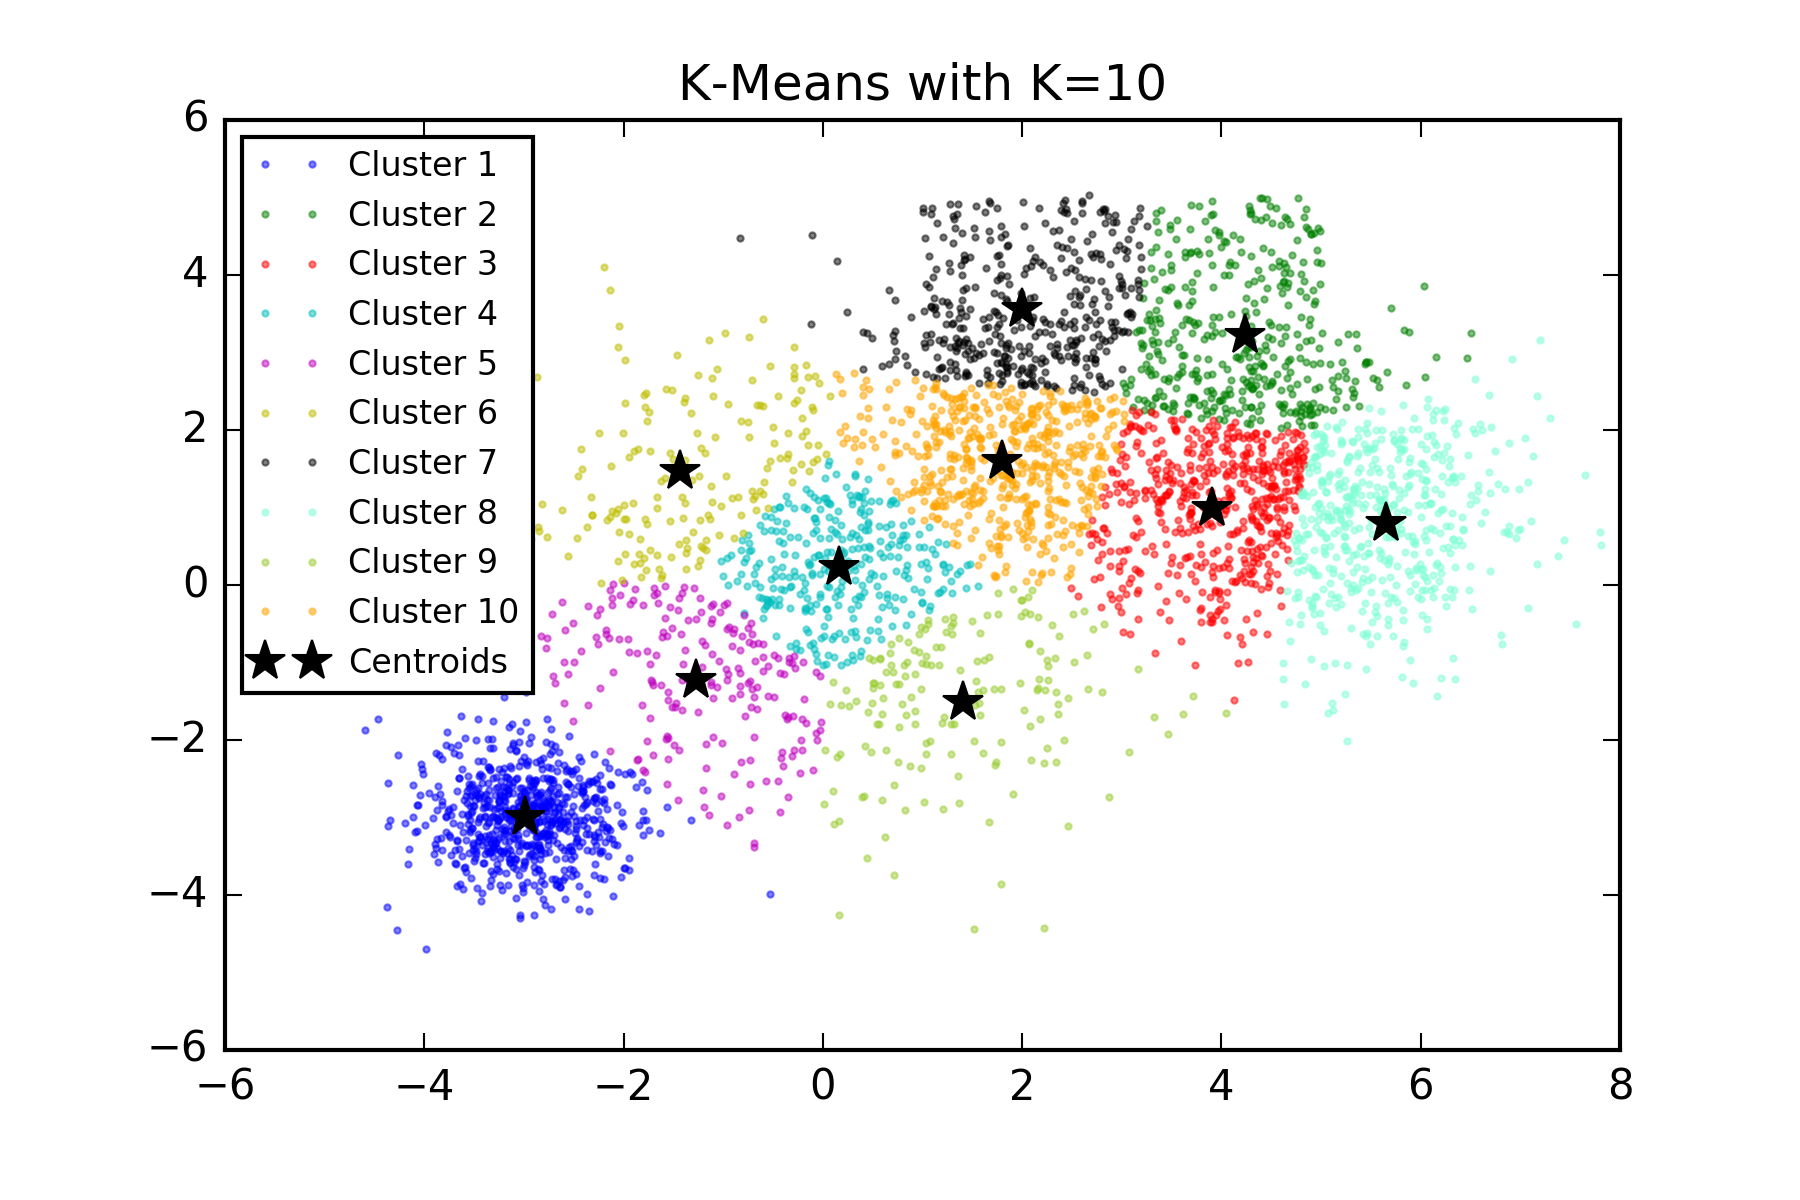
\includegraphics[width=\textwidth]{./figures/bigClustering_kMeans_10.png}
        \end{subfigure}
        
        \caption{Clustering Result for bigClusteringData.txt with K-Means Algorithm}
        \label{fig:kmean_clustering}
\end{figure}

%  -----------------------------------------------------------------------------
\begin{figure}[H]
\centering
\centering
        \begin{subfigure}[b]{0.49\textwidth}
            \centering
            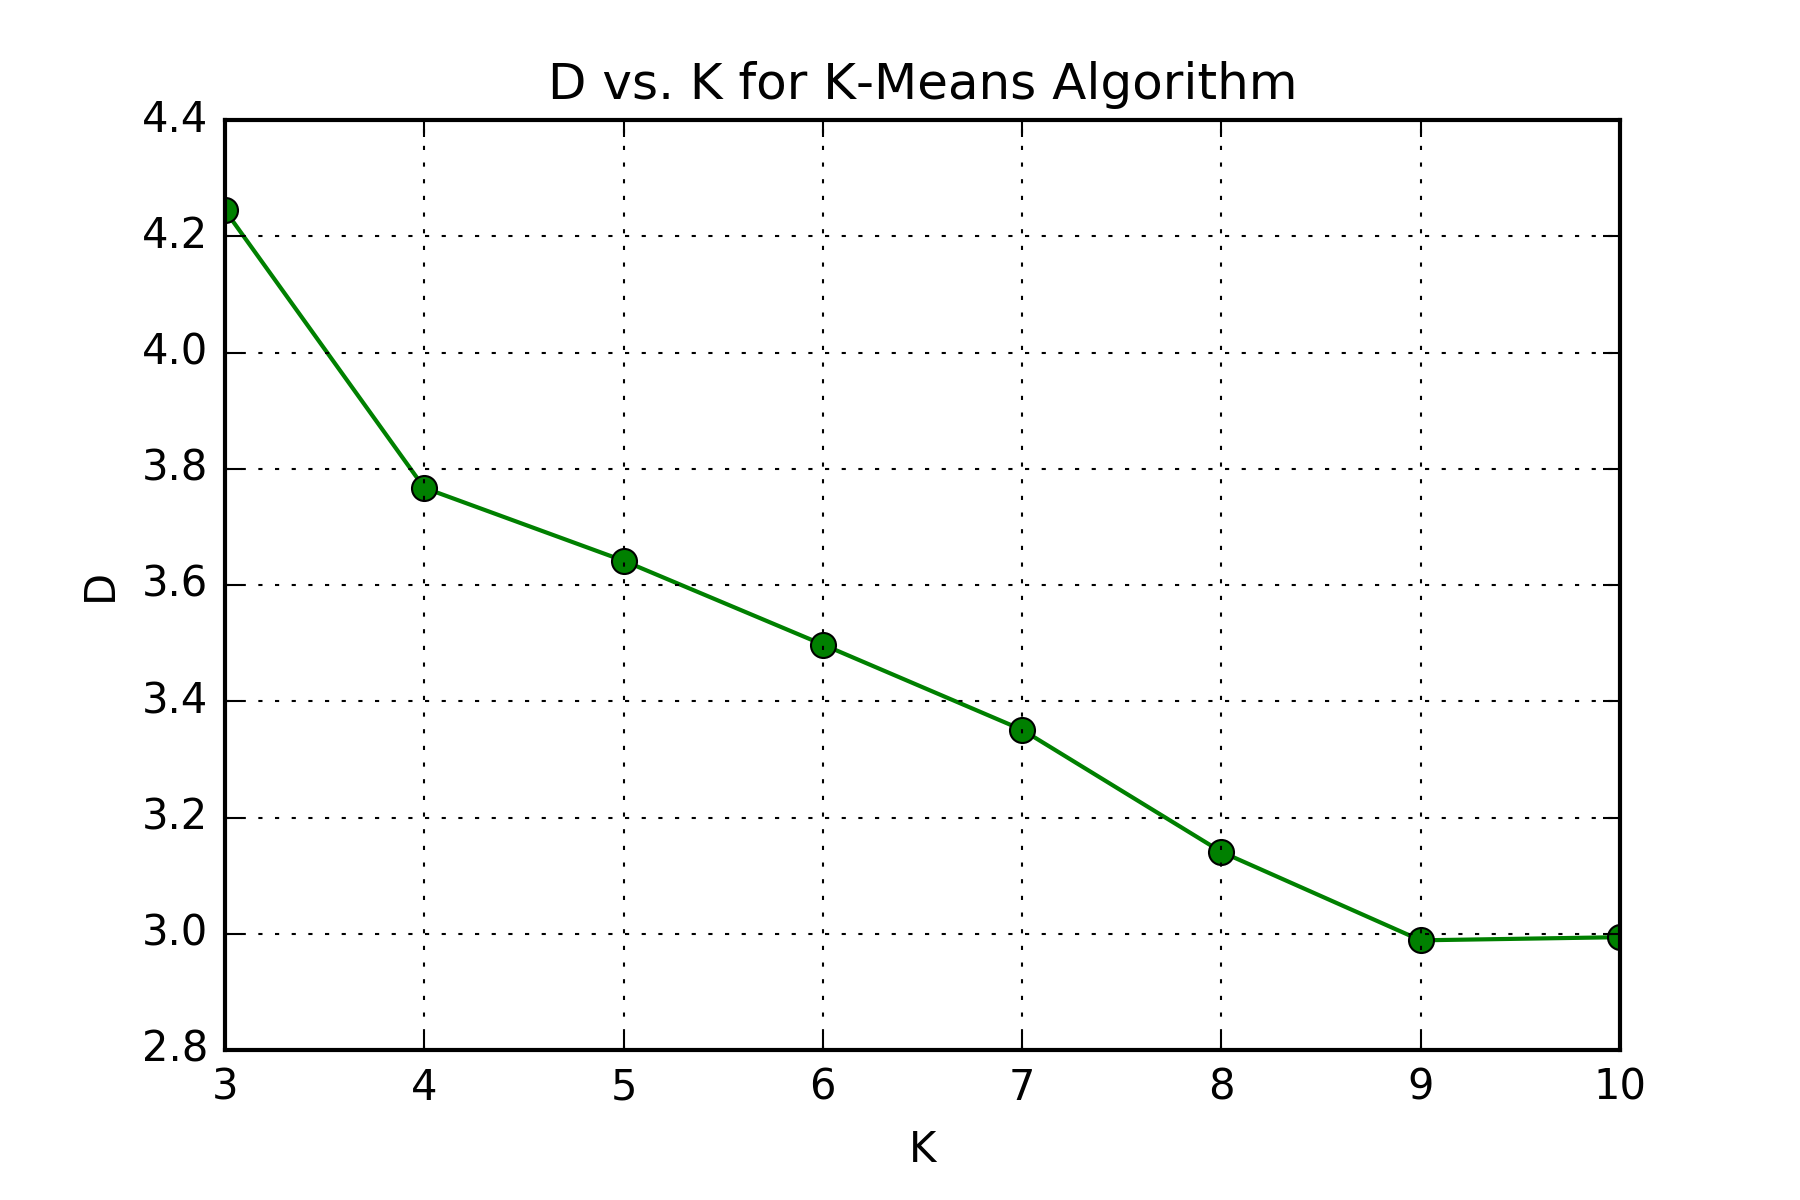
\includegraphics[width=\textwidth]{./figures/loss_clustering_kMeans.png}
            \caption{clustering.txt}\label{fig:3a}
        \end{subfigure}
        \hfill
        \begin{subfigure}[b]{0.49\textwidth}  
            \centering 
            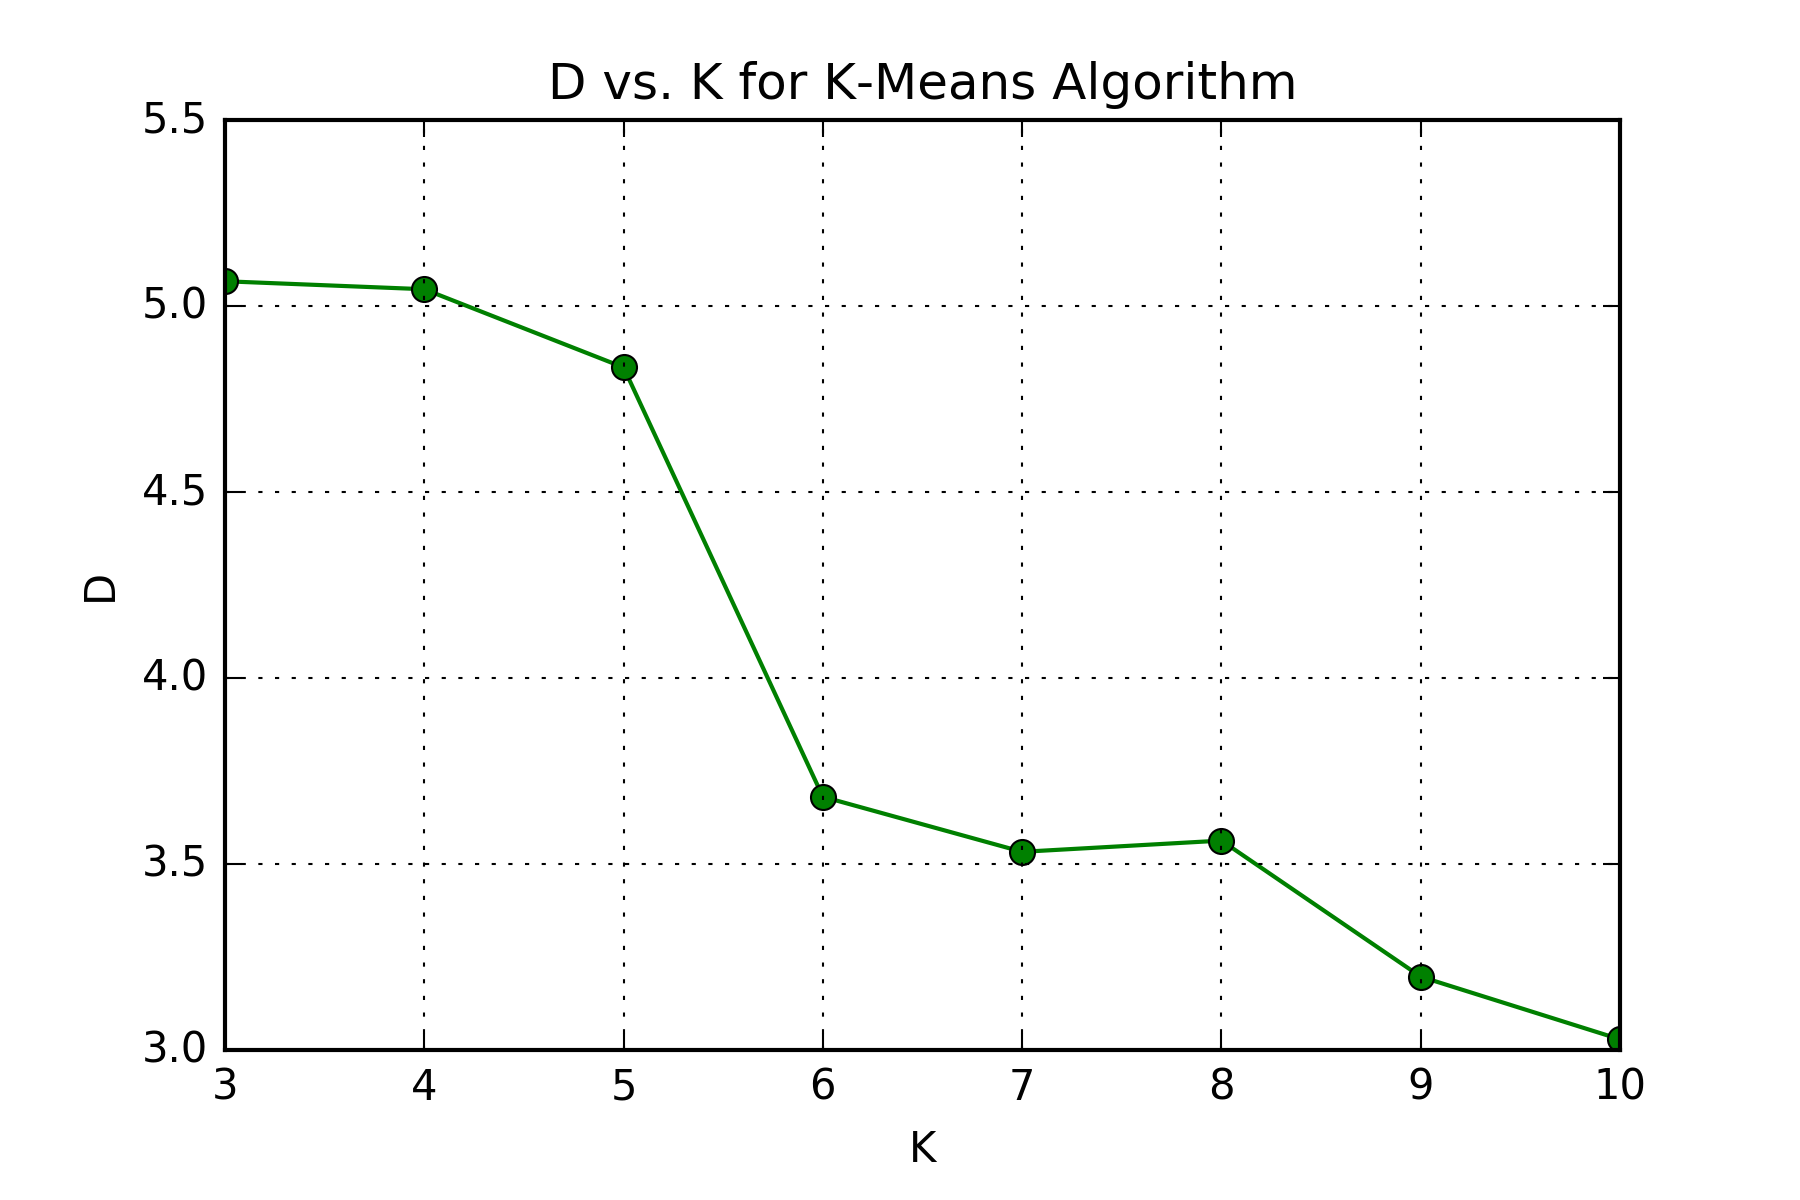
\includegraphics[width=\textwidth]{./figures/loss_bigClustering_kMeans.png}
            \caption{bigClusteringData.txt}\label{fig:3b}
        \end{subfigure}
\caption{Change of Distoration versus Cluster Number K for K-Means Algorithm}
\label{fig:k-means-loss} 
\end{figure}

% -----------------------------------------------------------------------------
\begin{lstlisting}[language=Python, caption=K-Means Algorithm Python Code]
import numpy as np
import time

def kMeans(X, K, tol=0.00001, random_state=None, verbose=True):
    """ function to implement the Lloyd's algorithm for k-means problem """
    np.random.seed(random_state)
    t0 = time.time()

    N, d = X.shape  # number of observations and dimensions
    index = np.random.choice(range(N), size=K, replace=False)
    Y = X[index, :]  # initial k centers
    C = np.zeros(N)
    D = 100
    count = 0
    diff = 100  # difference between D1 and D0

    while diff >= tol:
        D0 = D
        for i in range(N):
            # assign centers to ith data
            C[i] = np.argmin(np.sum((Y - X[i, :]) ** 2, axis=1))

        D = 0
        # re-compute the new centers
        for j in range(K):
            Y[j, :] = np.mean(X[C == j, :], axis=0)

        # compute the loss
        loss = np.zeros((N, K))
        for i in range(K):
            loss[:, i] = np.sqrt(np.sum((X - Y[i, :])**2, axis=1))
        D = np.max(np.min(loss, axis=1))
        diff = abs(D - D0)
        count += 1

    if verbose is True:
        t = np.round(time.time() - t0, 4)
        print('K-Means finished in ' + str(t) + 's, ' + str(count) + ' iters')

    return Y, C, D
\end{lstlisting}

\end{description}

% -----------------------------------------------------------------------------
\section*{\Large \Romannum{2}. Greedy K-centers Algorithm}

%  -----------------------------------------------------------------------------
\begin{figure}[htb]
        \centering
        \begin{subfigure}[b]{0.475\textwidth}
            \centering
            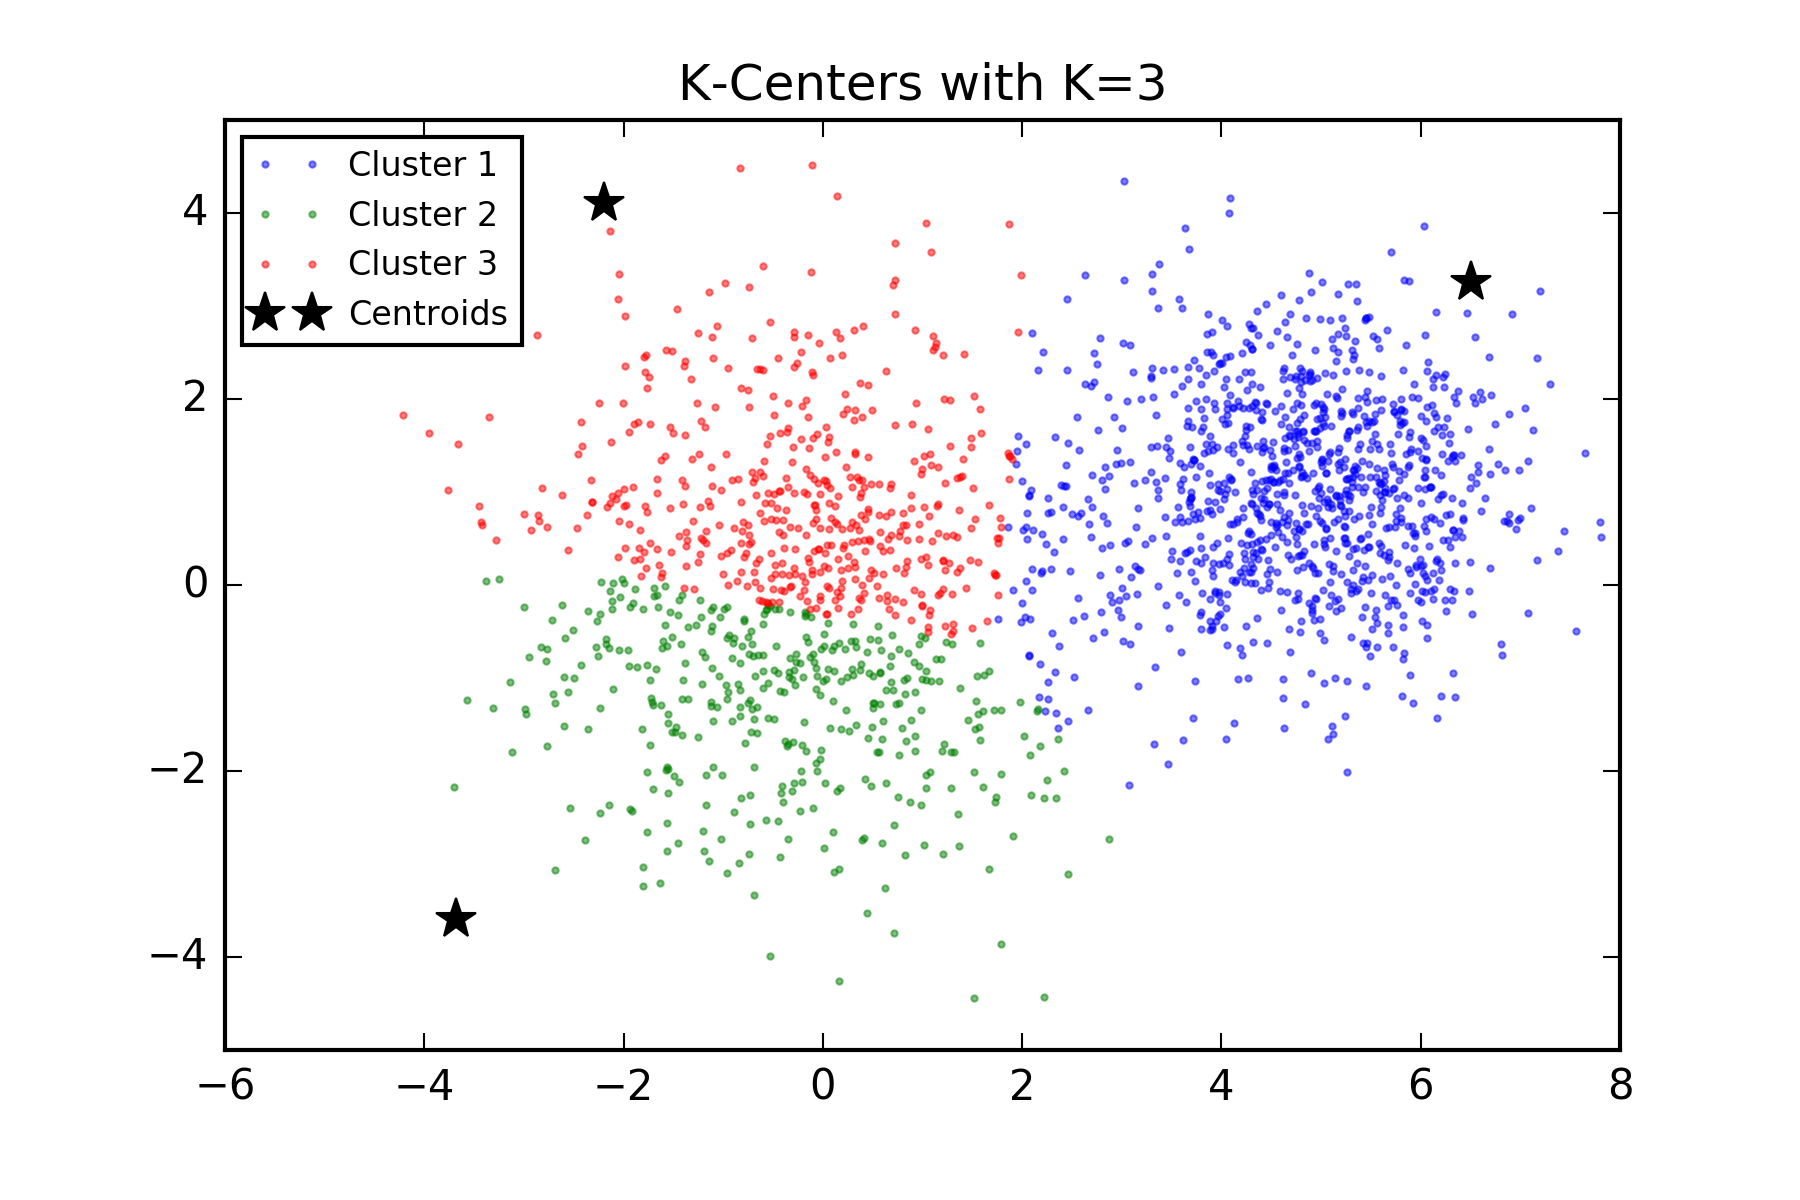
\includegraphics[width=\textwidth]{./figures/clustering_kCenter_3.png}
        \end{subfigure}
        \hfill
        \begin{subfigure}[b]{0.475\textwidth}  
            \centering 
            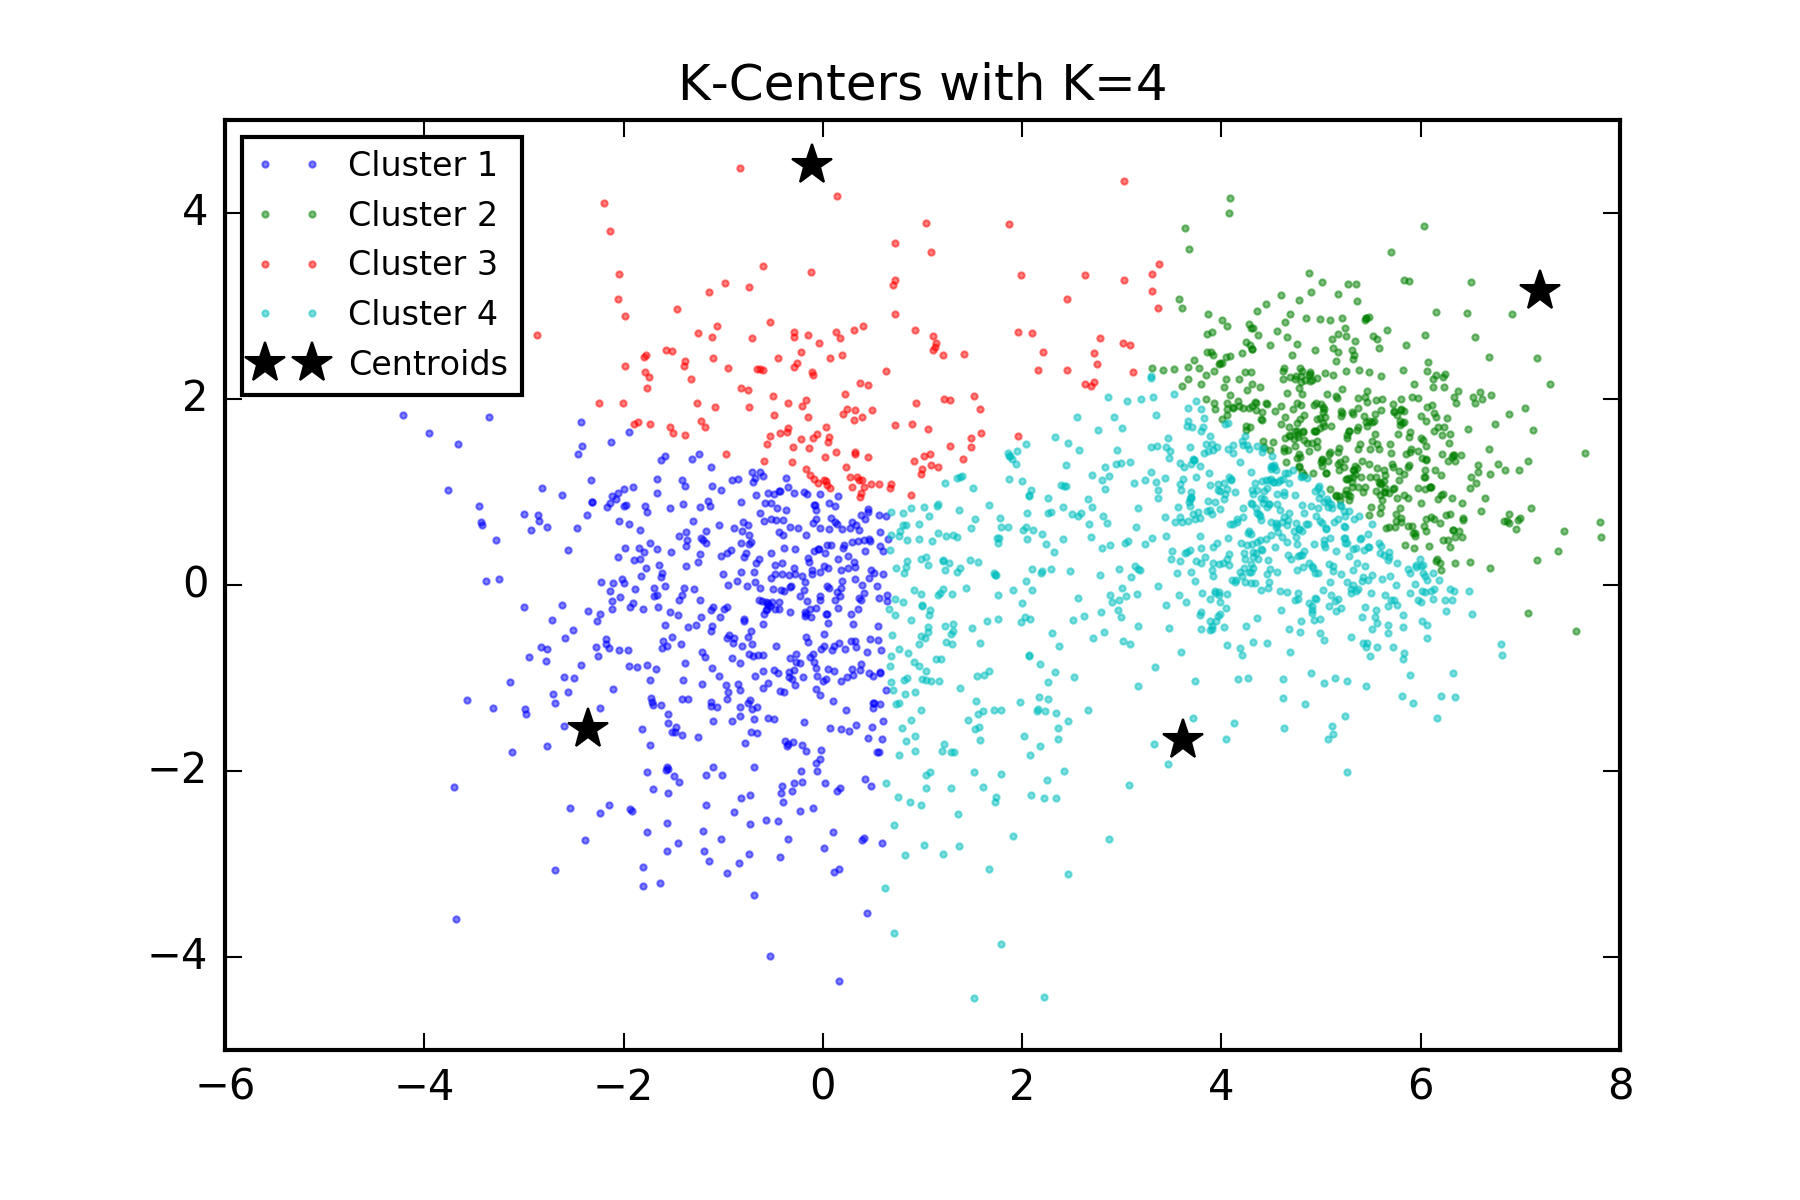
\includegraphics[width=\textwidth]{./figures/clustering_kCenter_4.png}
        \end{subfigure}
%        \vskip\baselineskip        
        \begin{subfigure}[b]{0.475\textwidth}  
            \centering 
            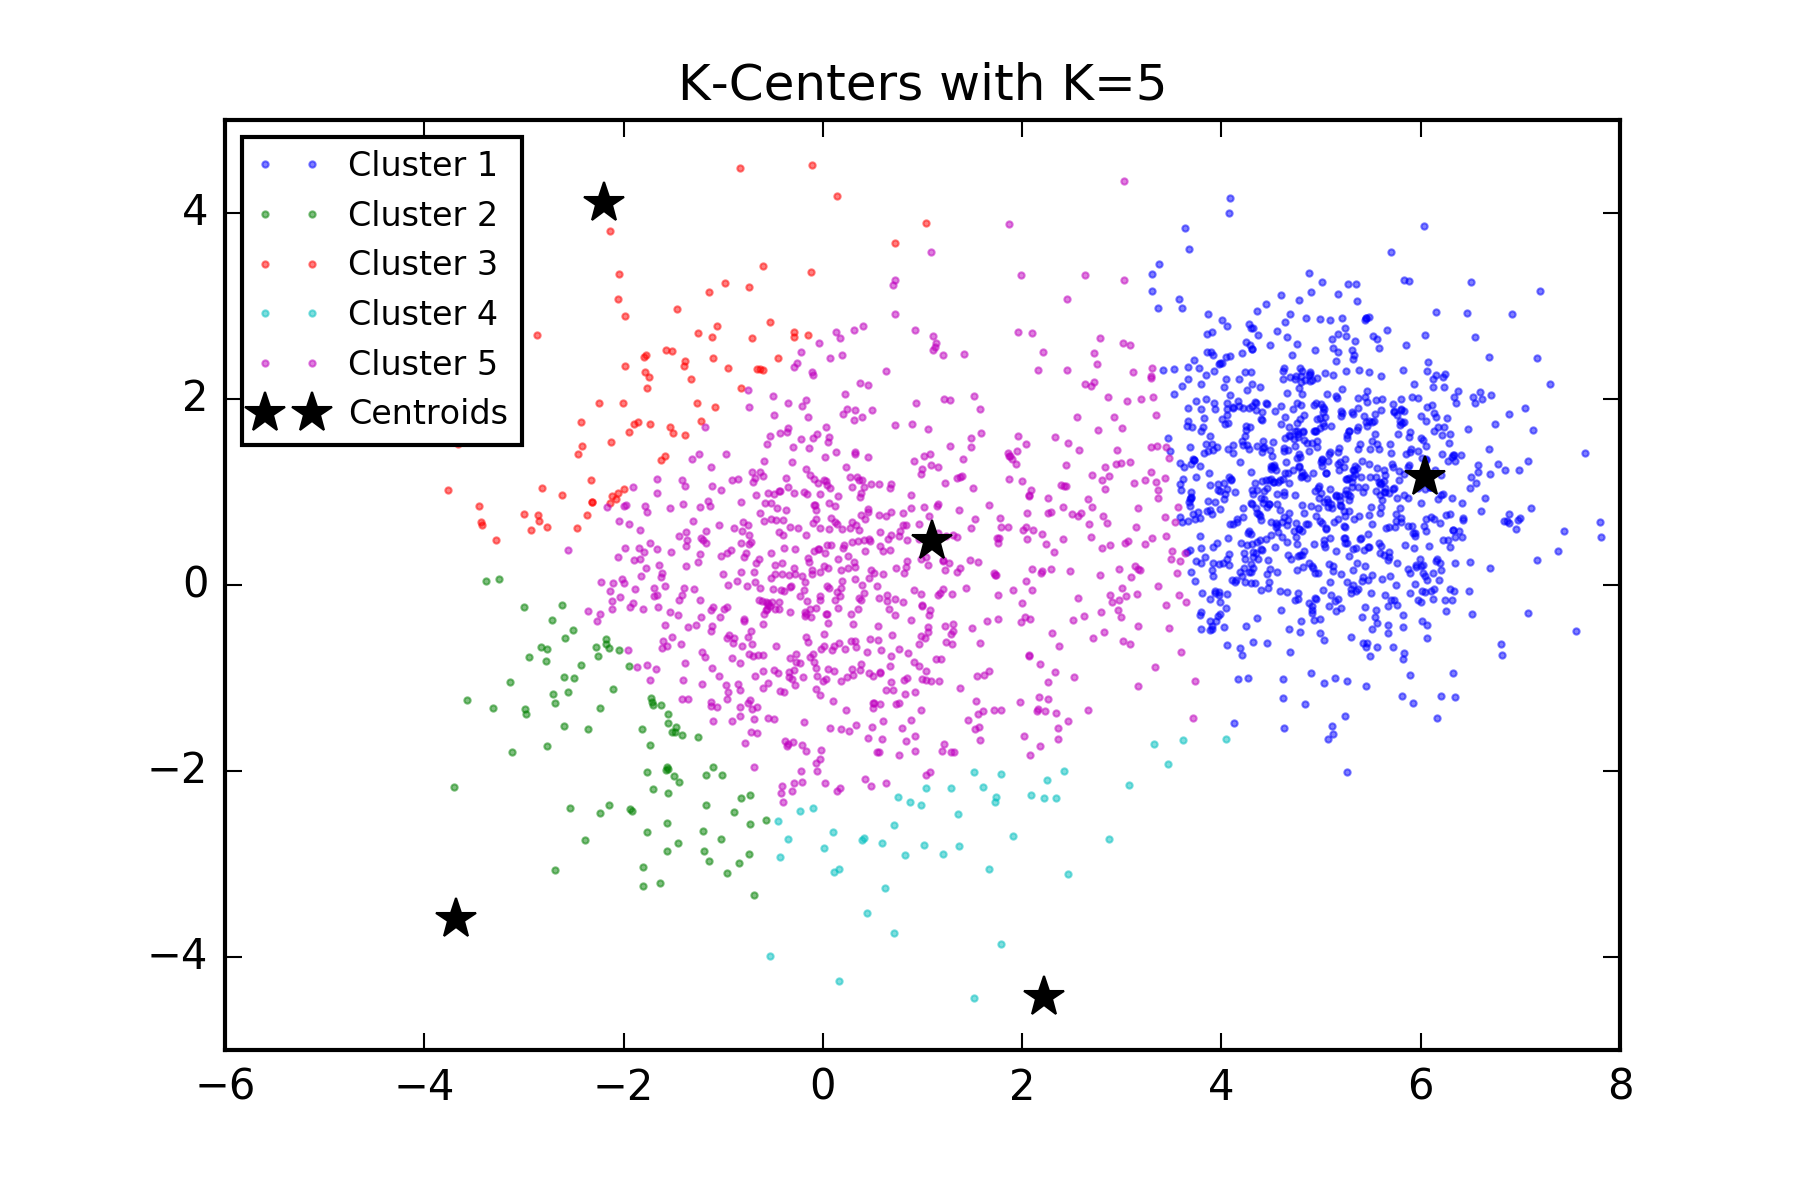
\includegraphics[width=\textwidth]{./figures/clustering_kCenter_5.png}
        \end{subfigure}
        \hfill
        \begin{subfigure}[b]{0.475\textwidth}   
            \centering 
            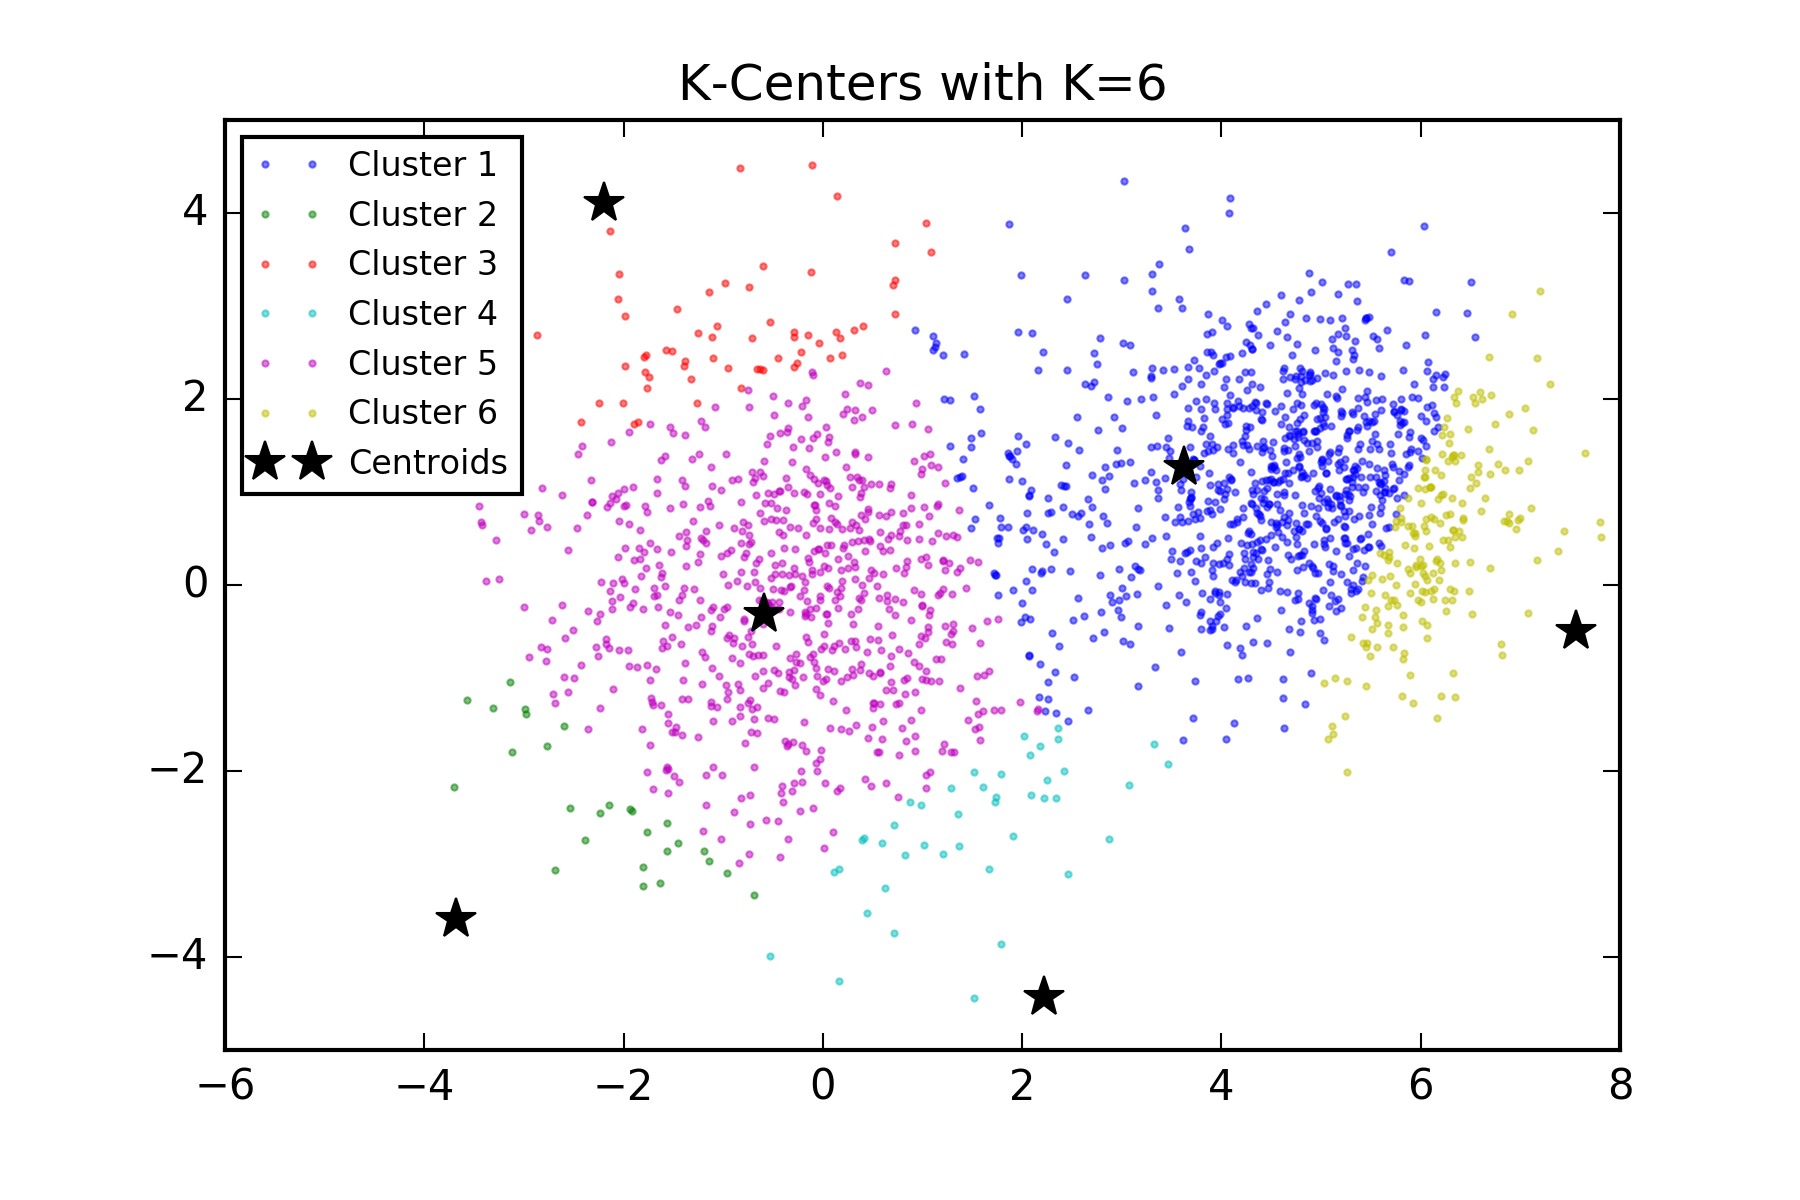
\includegraphics[width=\textwidth]{./figures/clustering_kCenter_6.png}
        \end{subfigure}
%        \vskip\baselineskip     
        \begin{subfigure}[b]{0.475\textwidth}   
            \centering 
            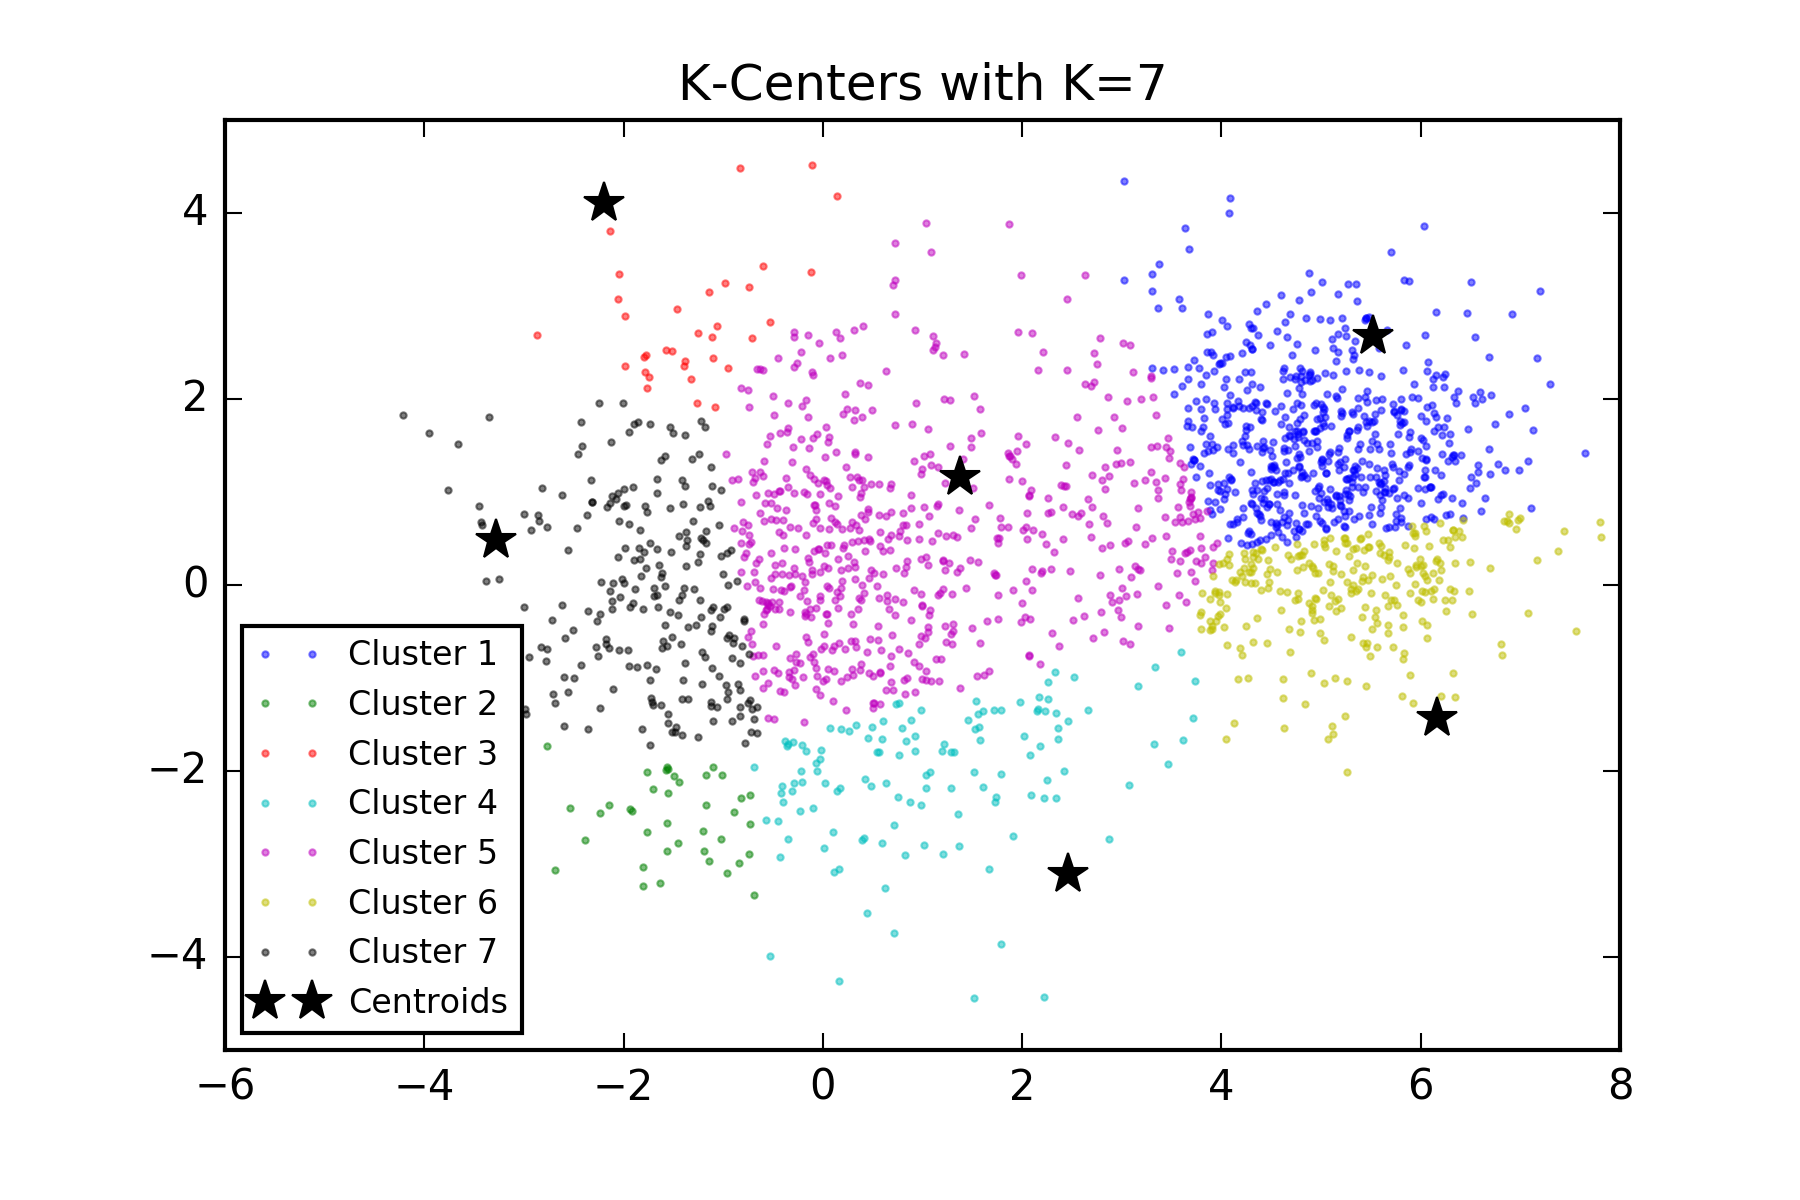
\includegraphics[width=\textwidth]{./figures/clustering_kCenter_7.png}
        \end{subfigure}
        \hfill
        \begin{subfigure}[b]{0.475\textwidth}  
            \centering 
            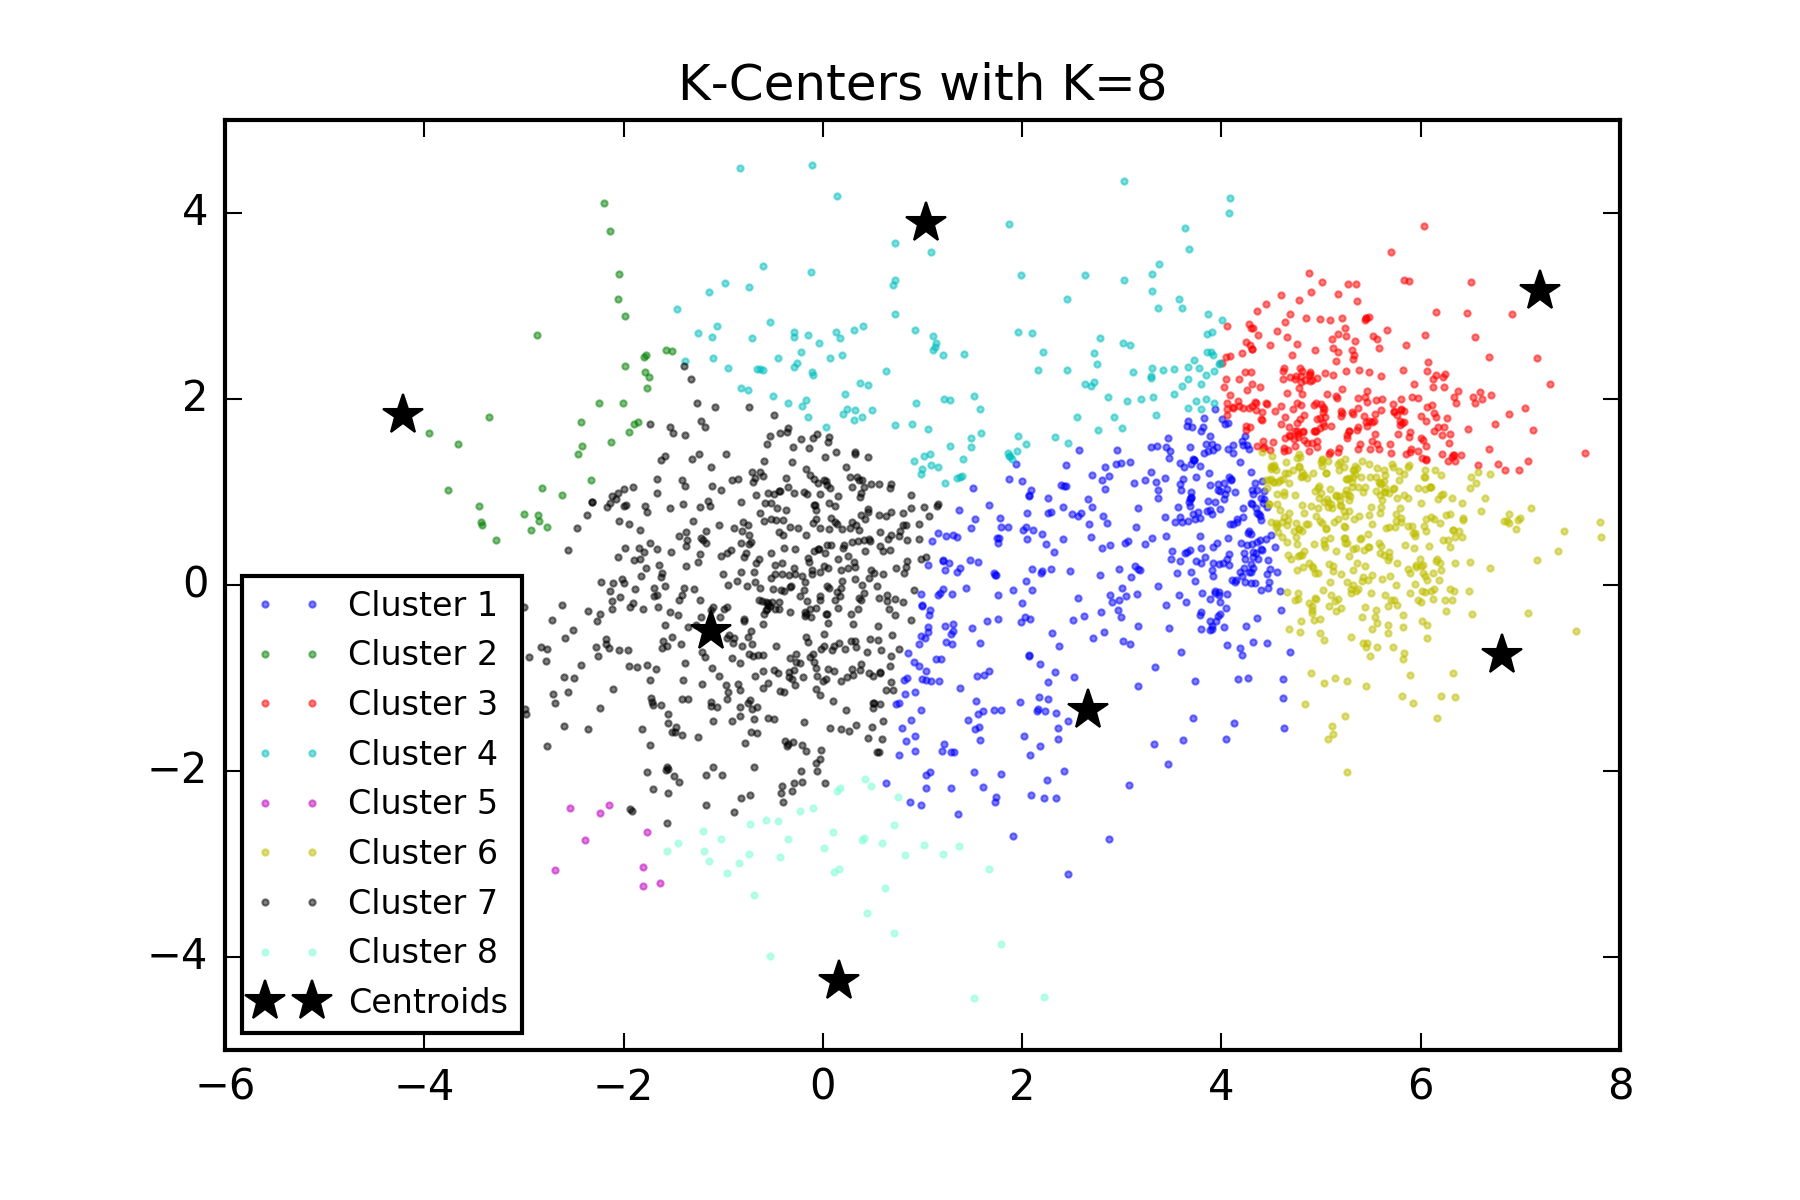
\includegraphics[width=\textwidth]{./figures/clustering_kCenter_8.png}
        \end{subfigure}
%        \vskip\baselineskip
        \begin{subfigure}[b]{0.475\textwidth}   
            \centering 
            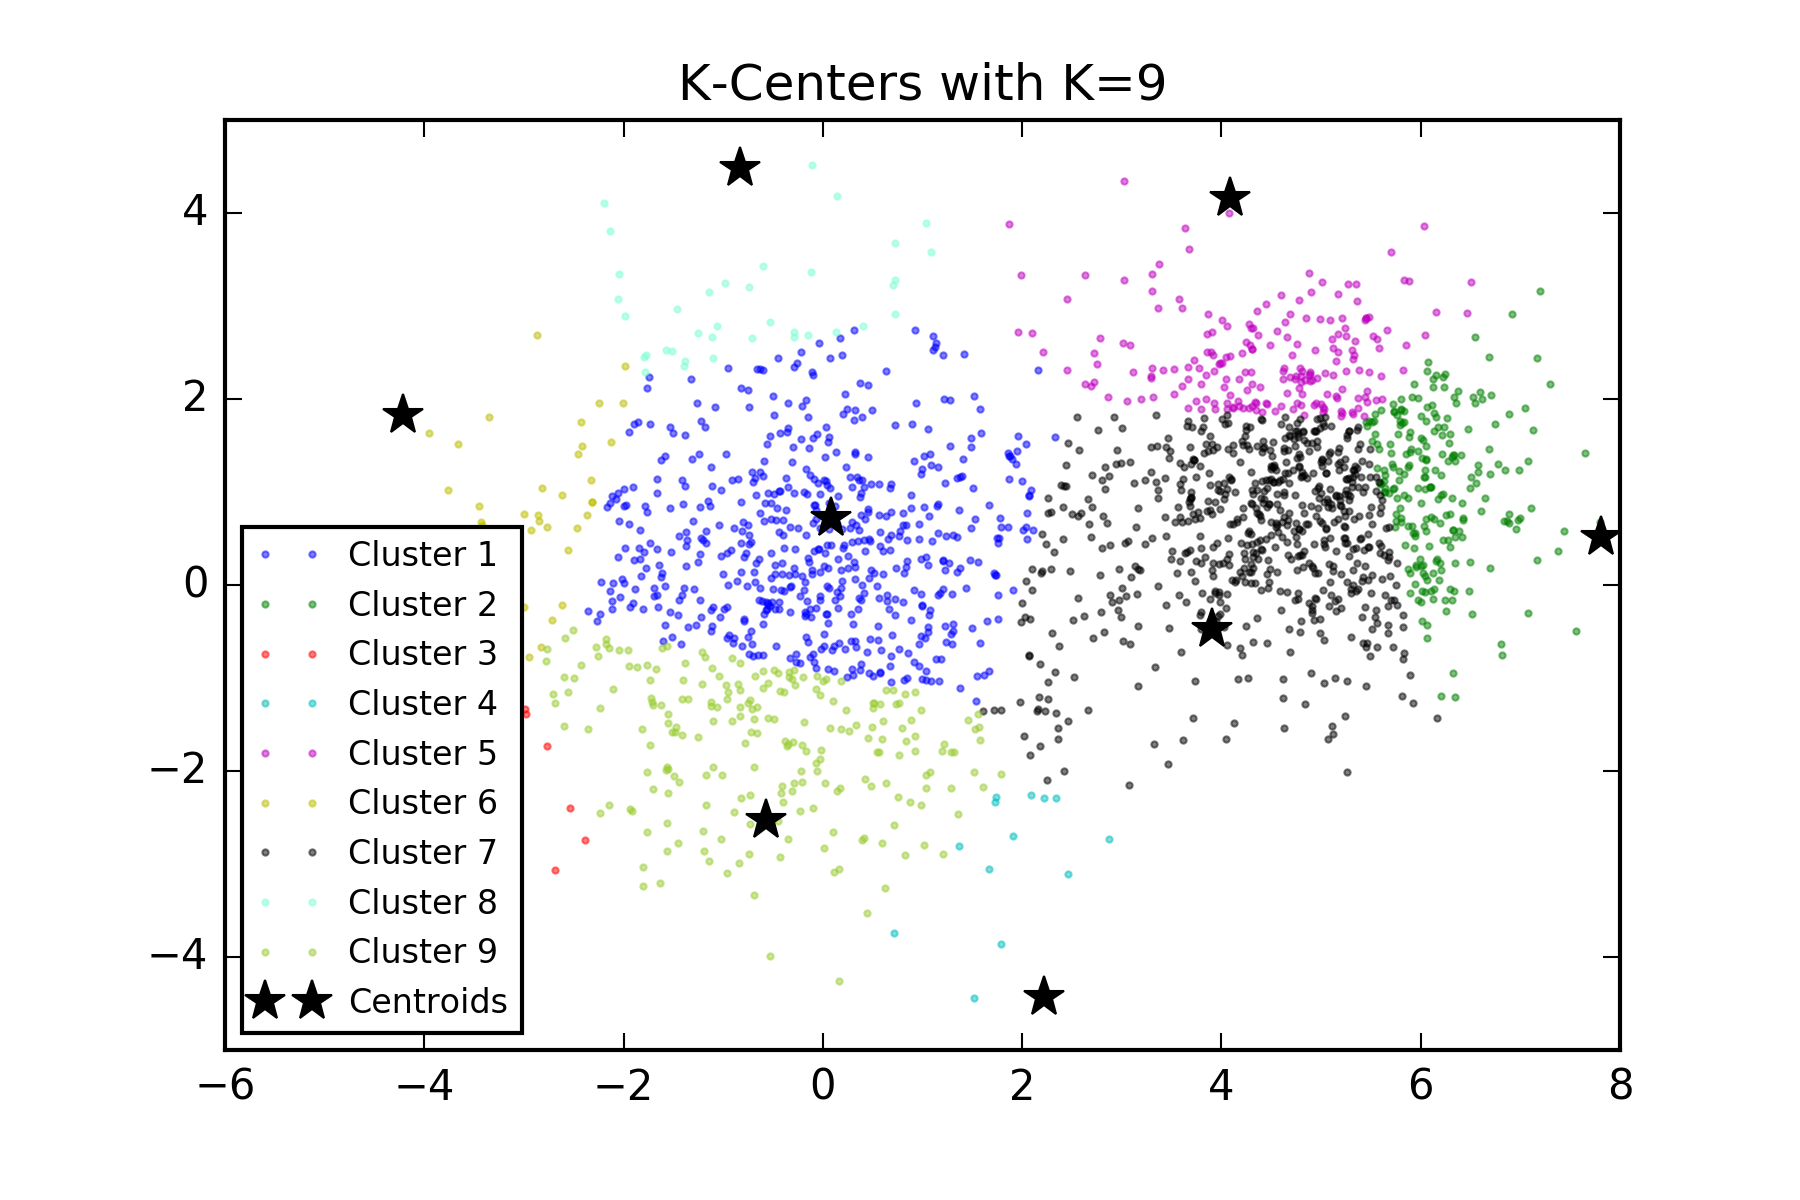
\includegraphics[width=\textwidth]{./figures/clustering_kCenter_9.png}
        \end{subfigure}
        \hfill
        \begin{subfigure}[b]{0.475\textwidth}   
            \centering 
            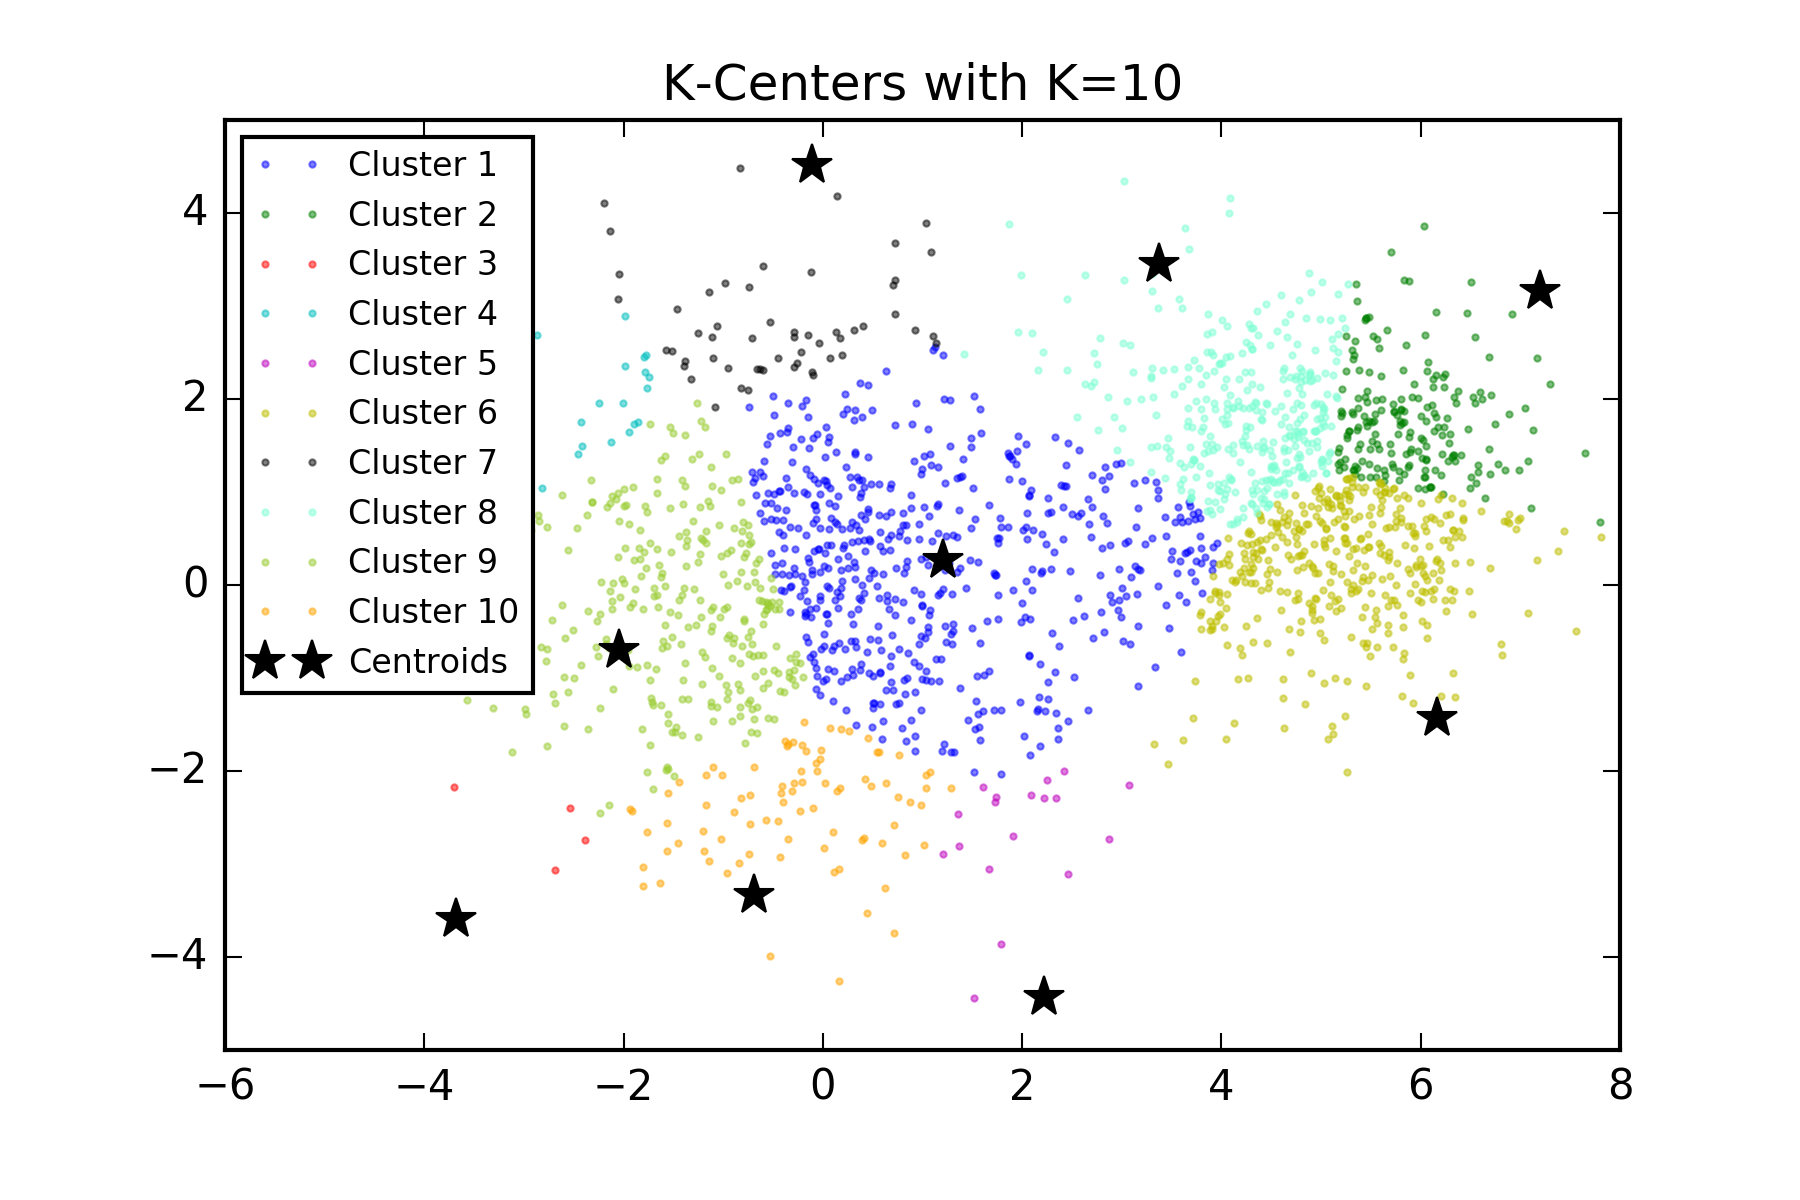
\includegraphics[width=\textwidth]{./figures/clustering_kCenter_10.png}
        \end{subfigure}
        
        \caption{Clustering Result for clustering.txt with K-Center Algorithm}
        \label{fig:kmean_clustering}
\end{figure}

%  -----------------------------------------------------------------------------
\begin{figure}[htb]
        \centering
        \begin{subfigure}[b]{0.475\textwidth}
            \centering
            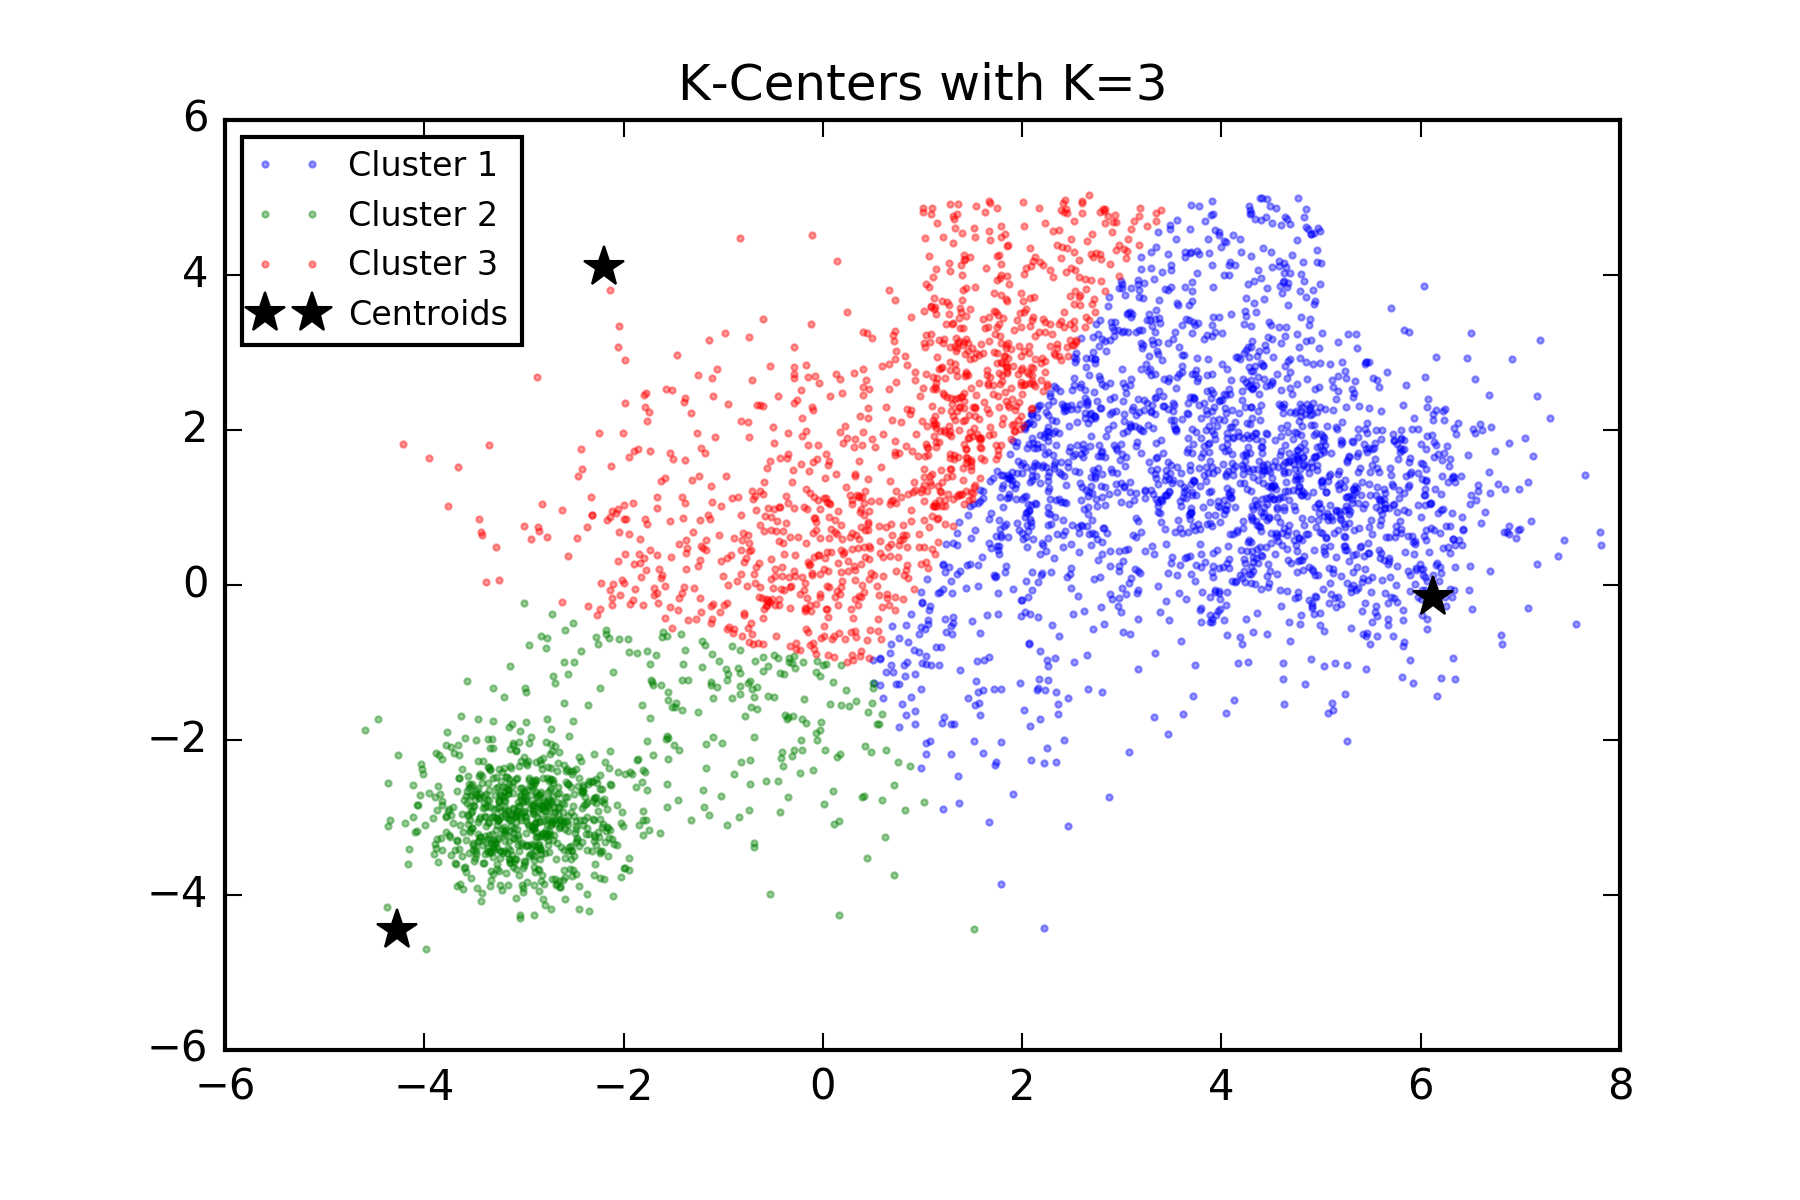
\includegraphics[width=\textwidth]{./figures/bigClustering_kCenter_3.png}
        \end{subfigure}
        \hfill
        \begin{subfigure}[b]{0.475\textwidth}  
            \centering 
            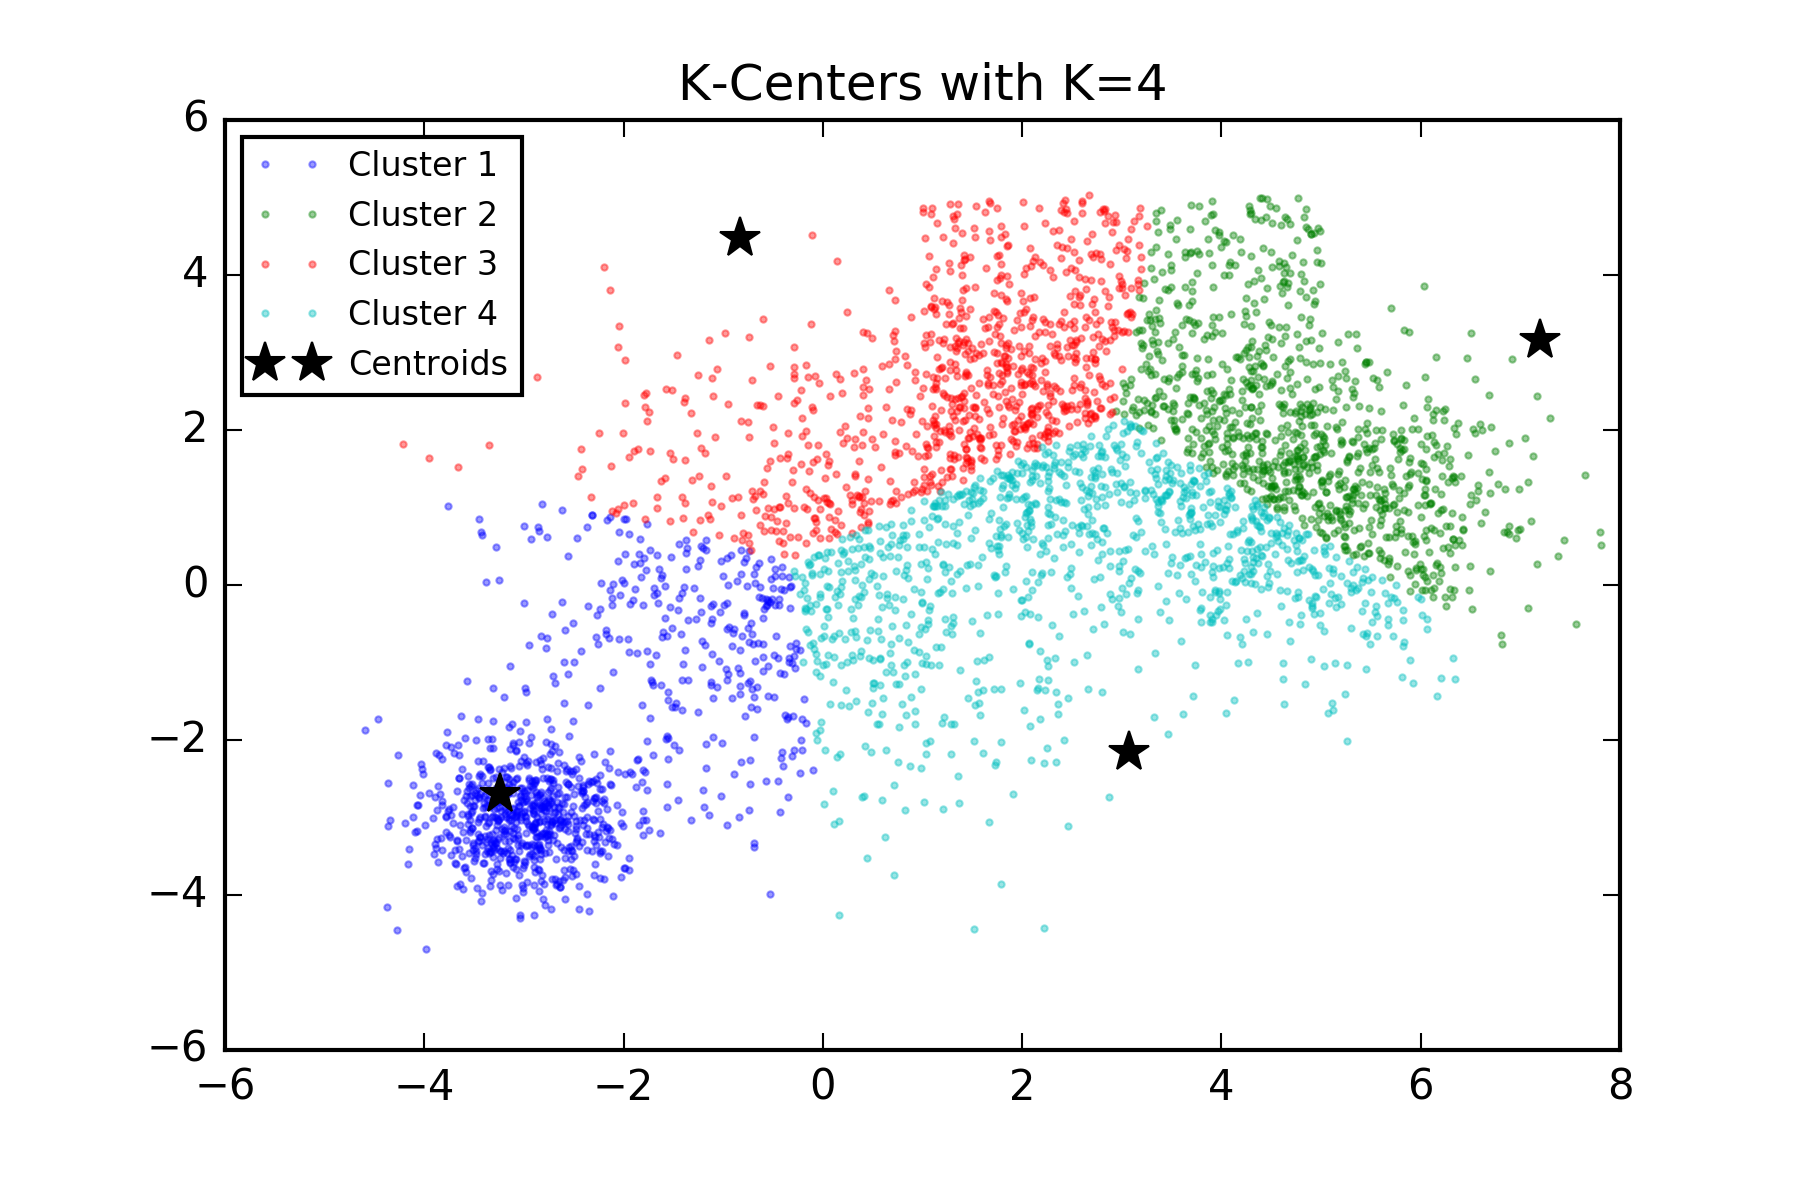
\includegraphics[width=\textwidth]{./figures/bigClustering_kCenter_4.png}
        \end{subfigure}
%        \vskip\baselineskip        
        \begin{subfigure}[b]{0.475\textwidth}  
            \centering 
            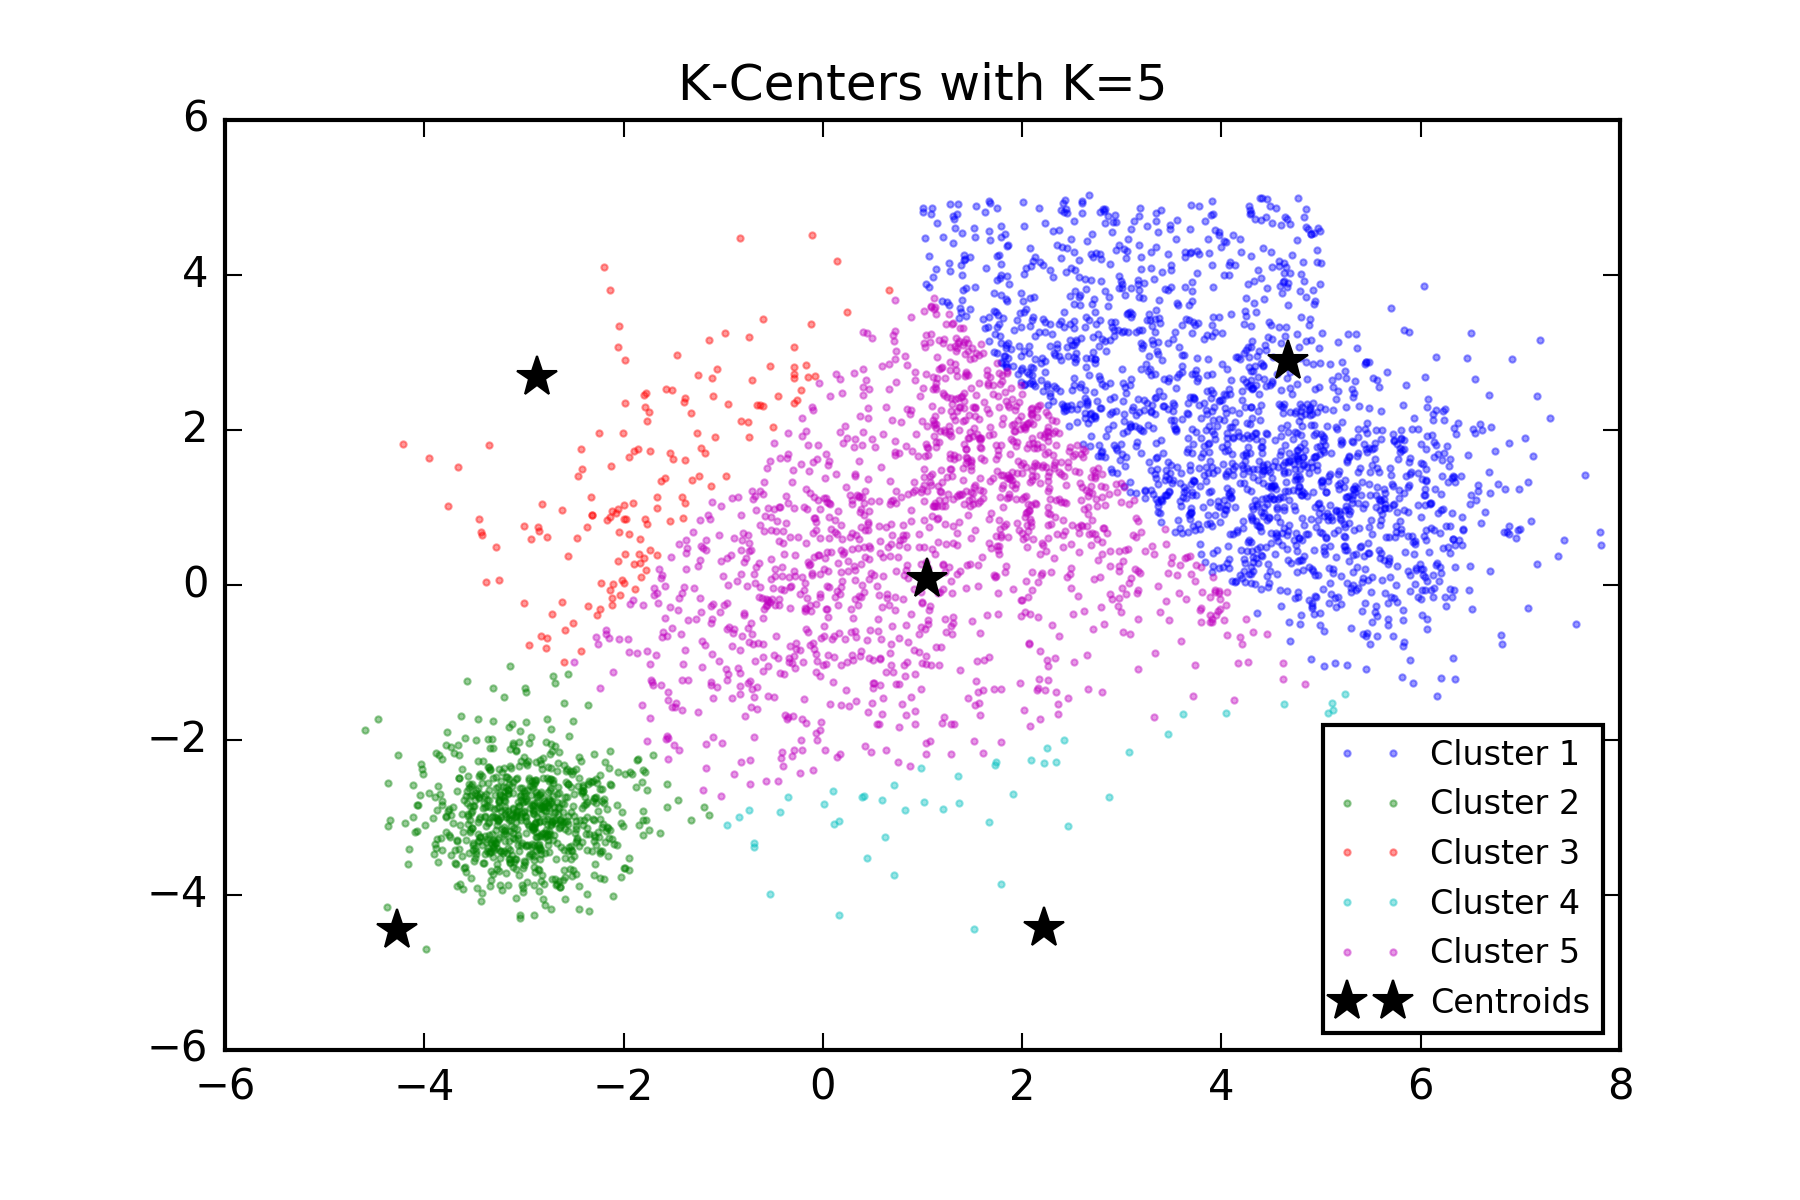
\includegraphics[width=\textwidth]{./figures/bigClustering_kCenter_5.png}
        \end{subfigure}
        \hfill
        \begin{subfigure}[b]{0.475\textwidth}   
            \centering 
            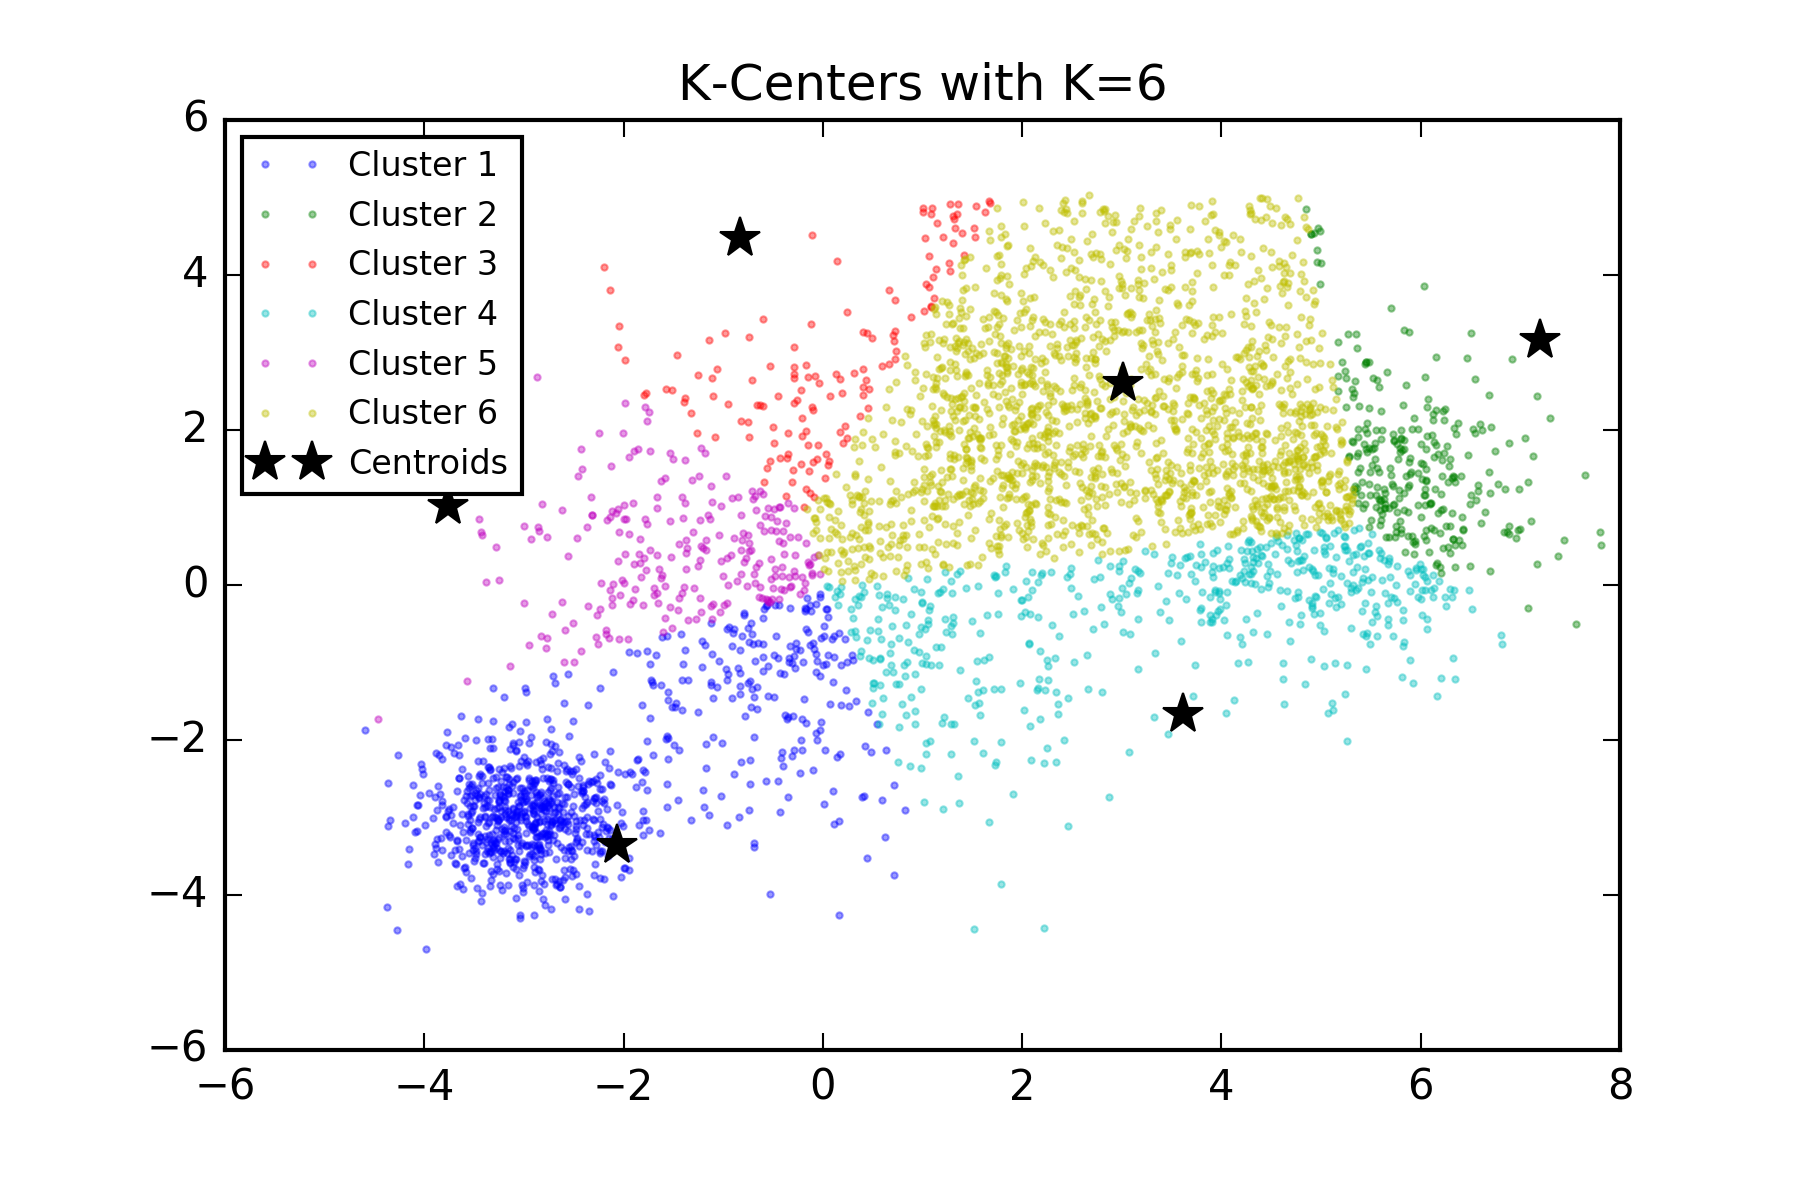
\includegraphics[width=\textwidth]{./figures/bigClustering_kCenter_6.png}
        \end{subfigure}
%        \vskip\baselineskip     
        \begin{subfigure}[b]{0.475\textwidth}   
            \centering 
            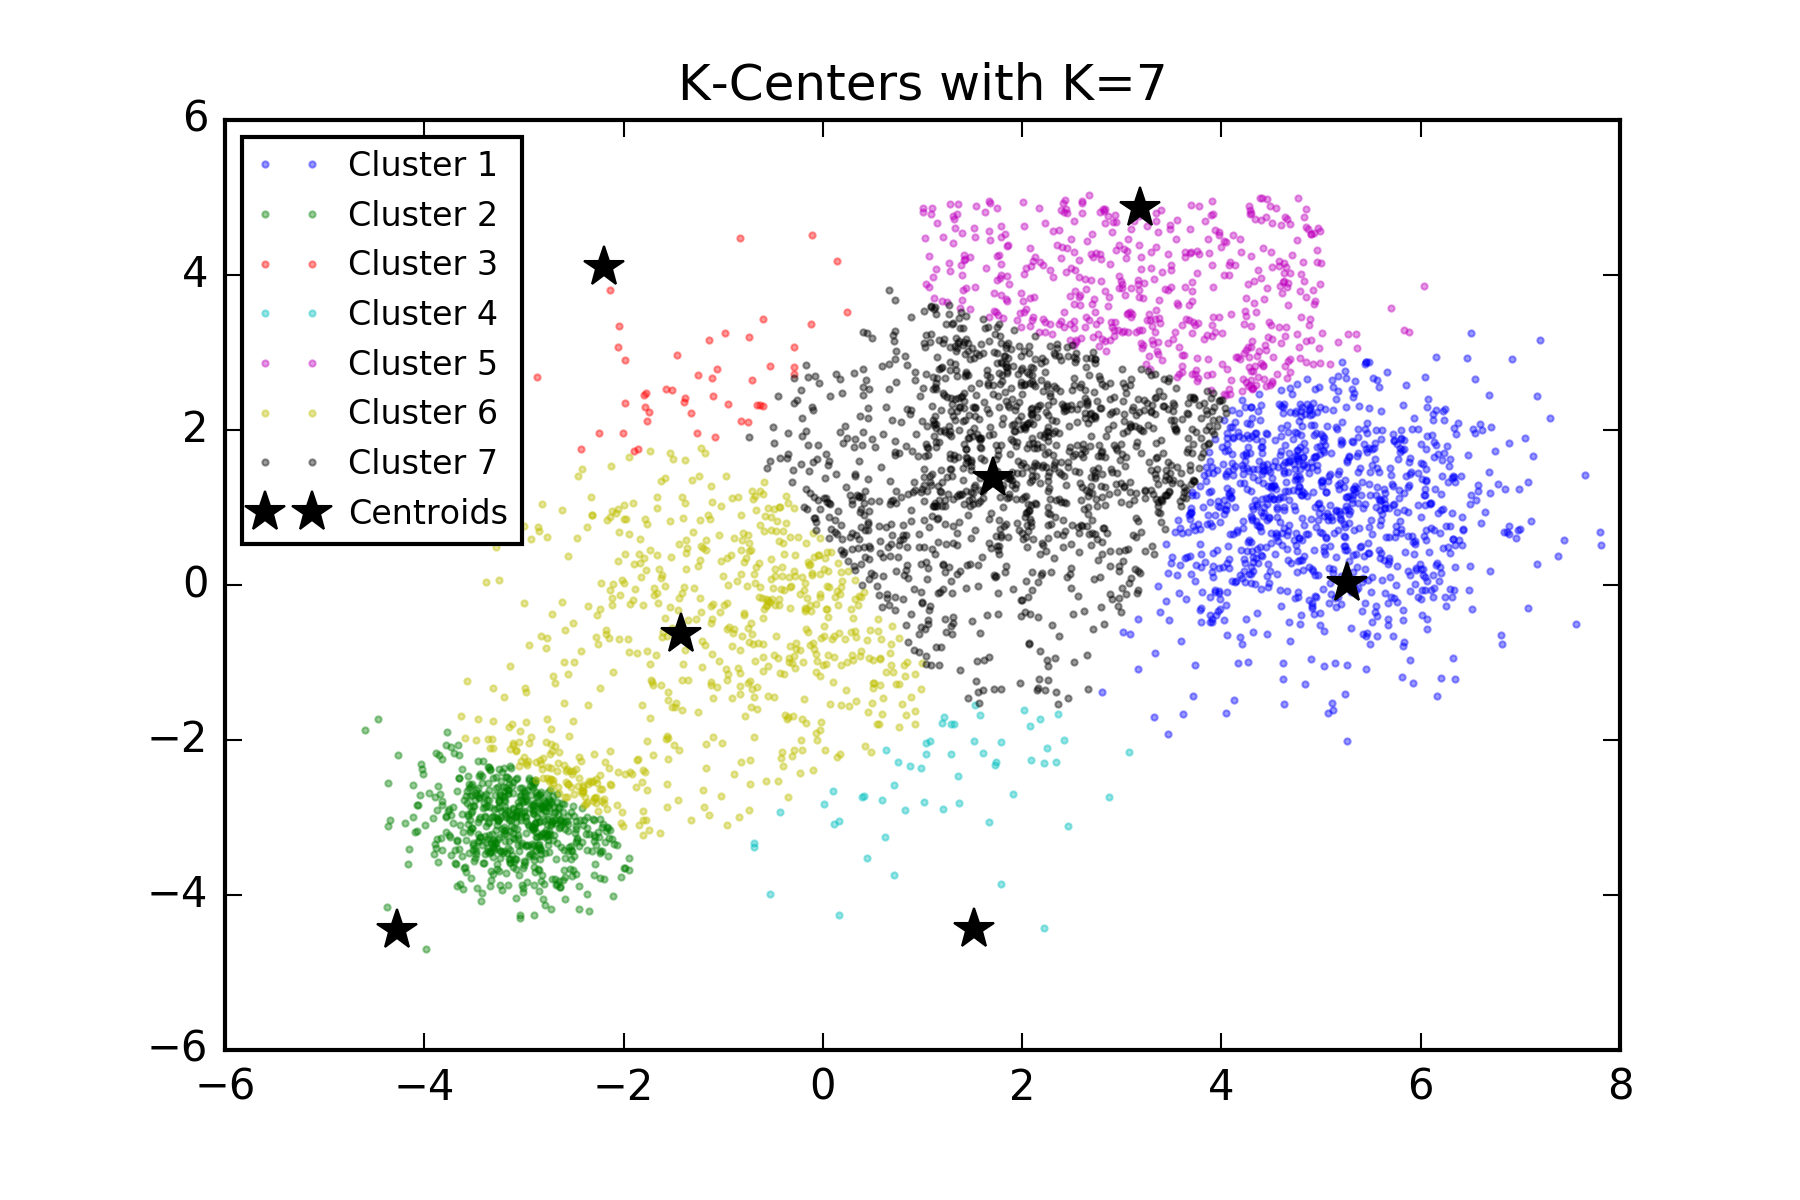
\includegraphics[width=\textwidth]{./figures/bigClustering_kCenter_7.png}
        \end{subfigure}
        \hfill
        \begin{subfigure}[b]{0.475\textwidth}  
            \centering 
            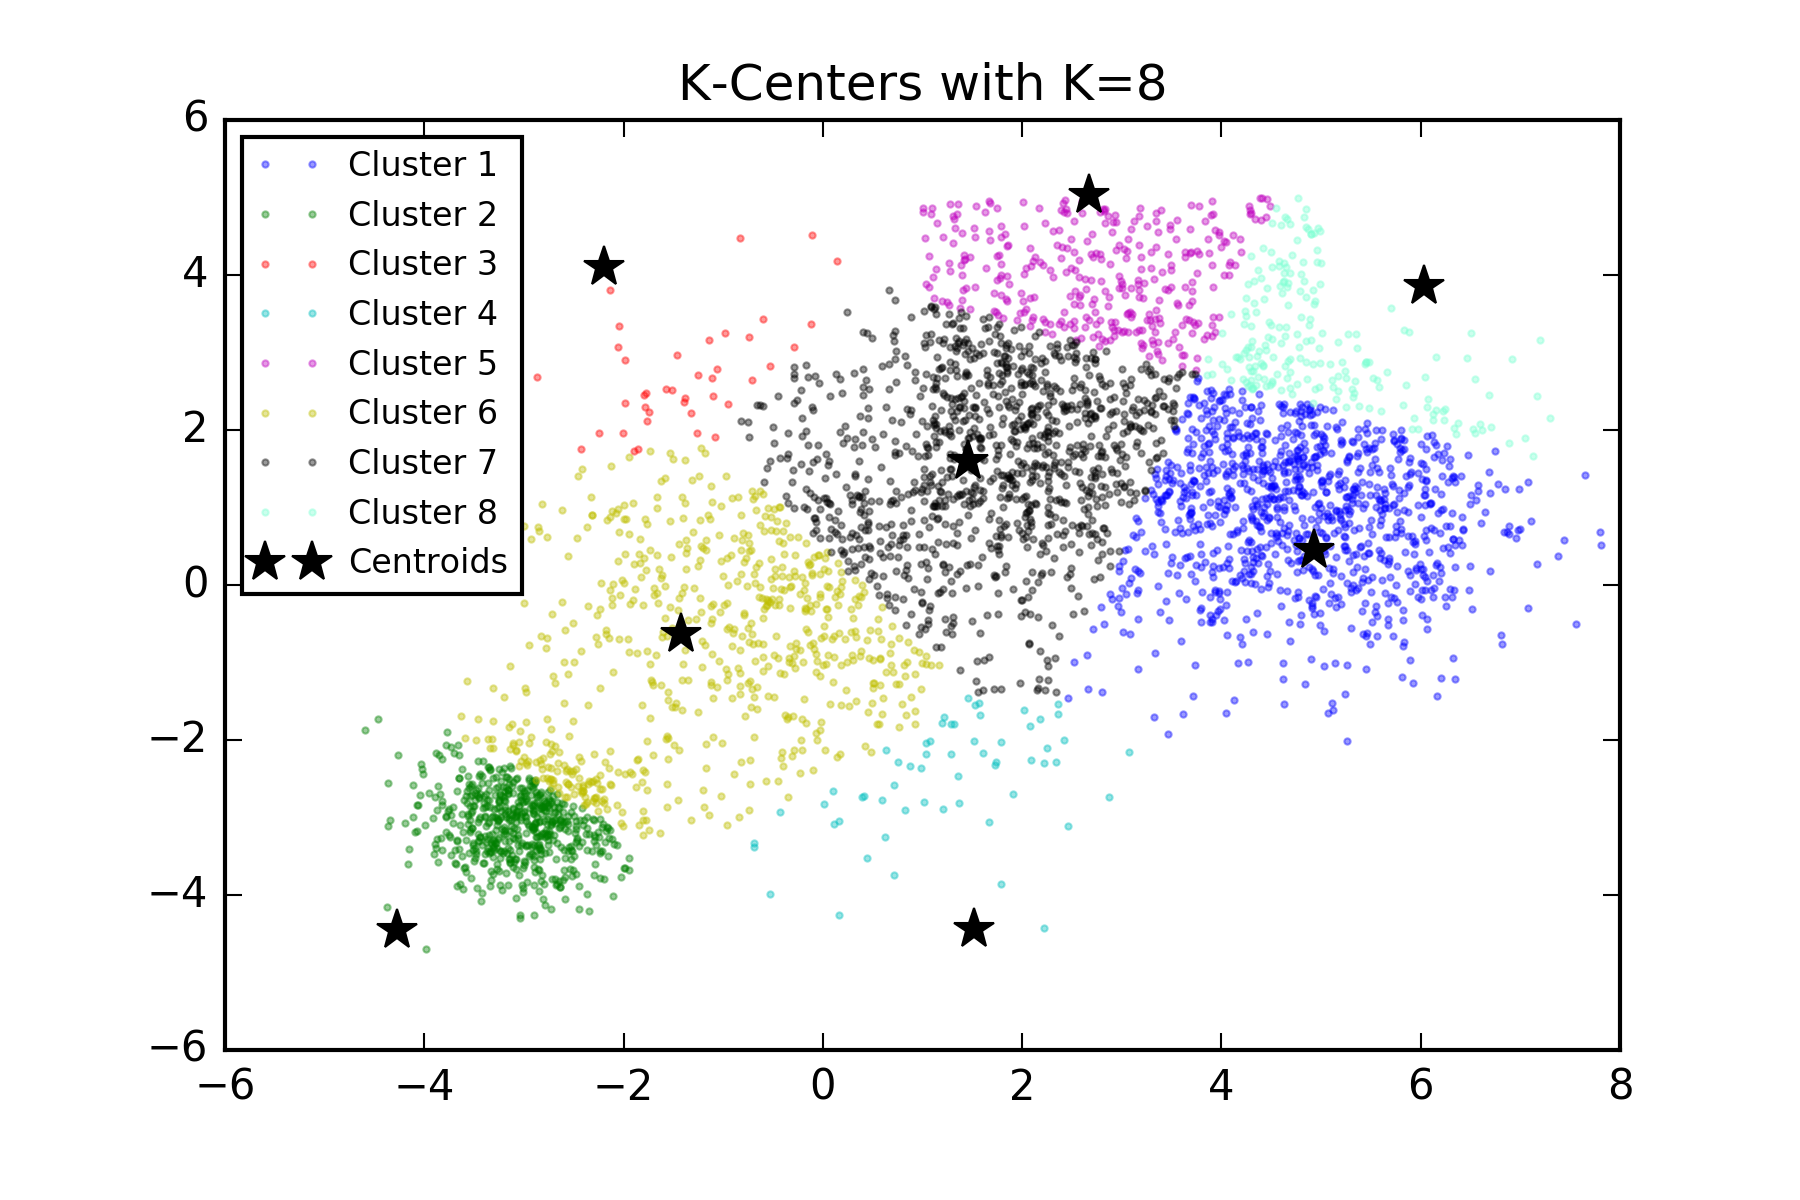
\includegraphics[width=\textwidth]{./figures/bigClustering_kCenter_8.png}
        \end{subfigure}
%        \vskip\baselineskip
        \begin{subfigure}[b]{0.475\textwidth}   
            \centering 
            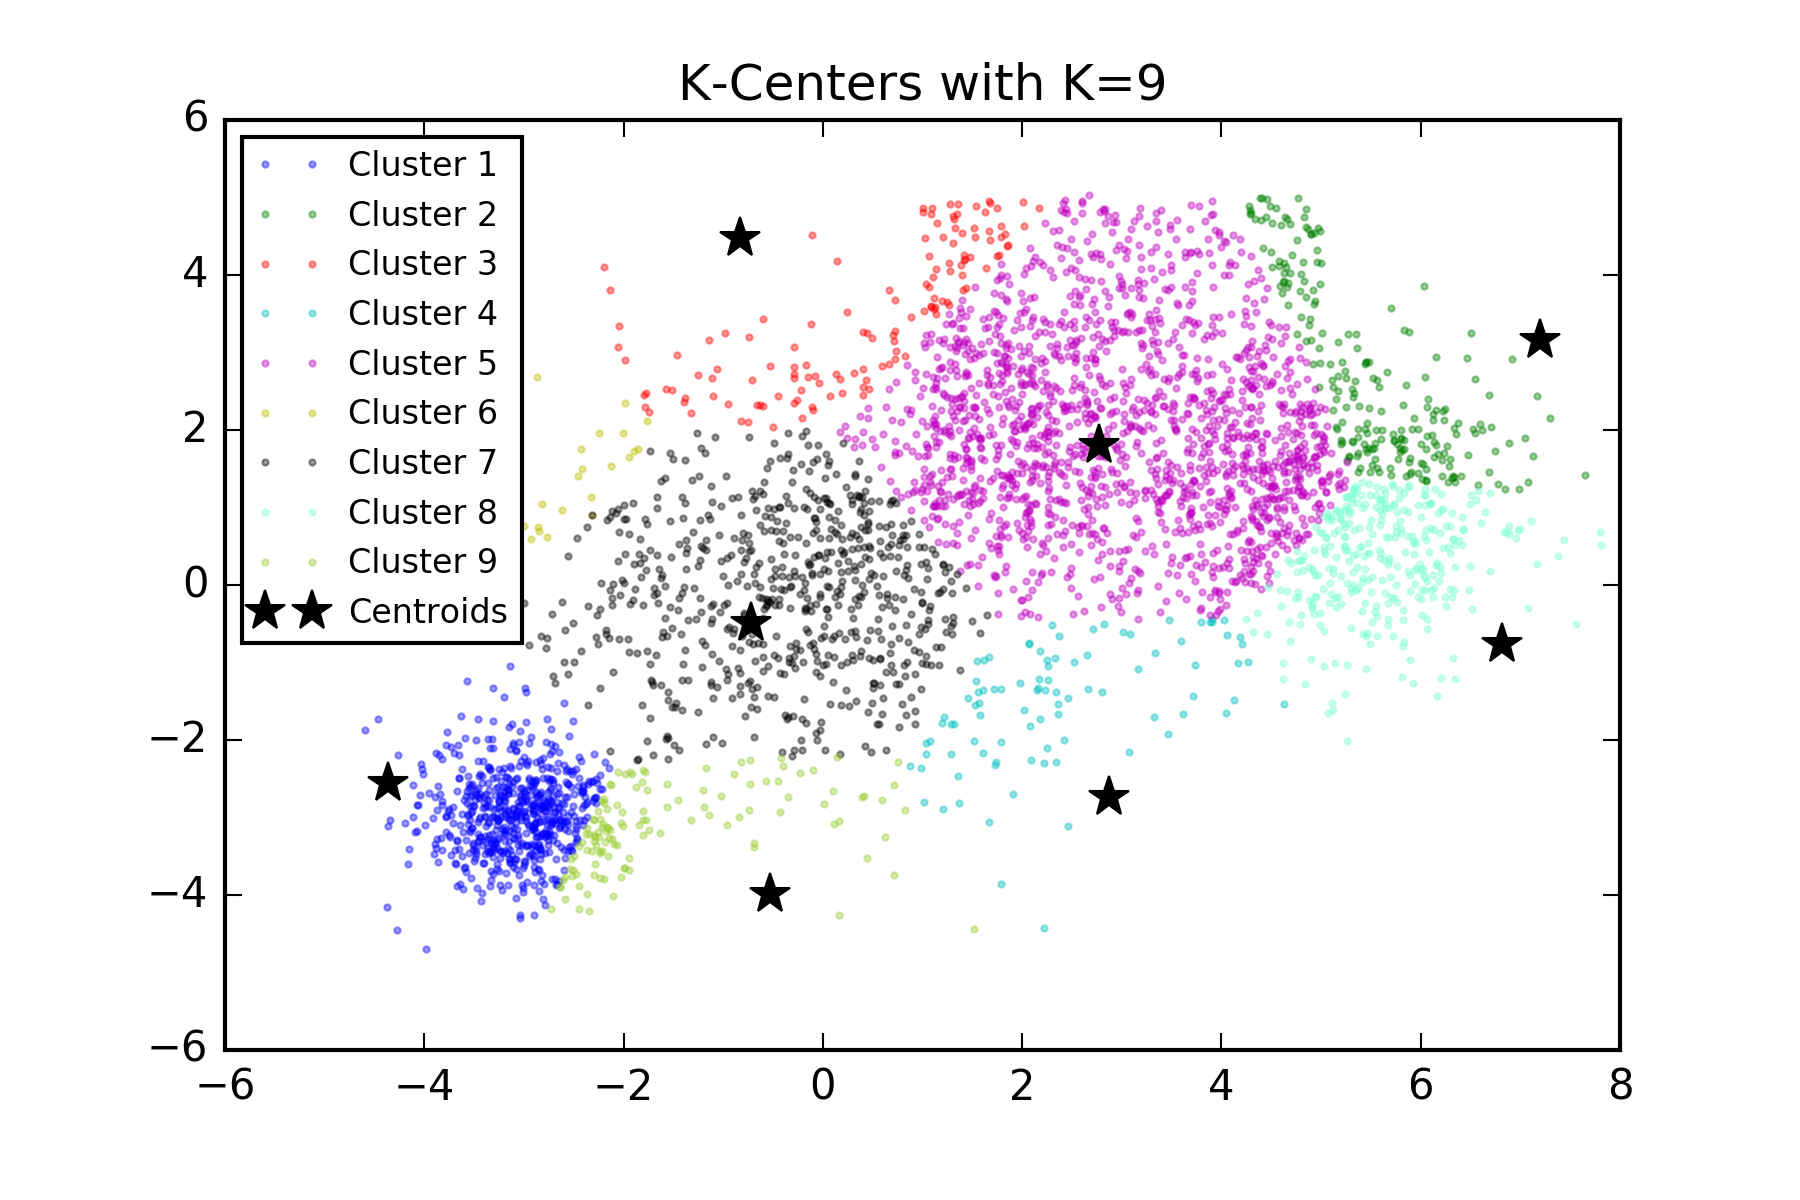
\includegraphics[width=\textwidth]{./figures/bigClustering_kCenter_9.png}
        \end{subfigure}
        \hfill
        \begin{subfigure}[b]{0.475\textwidth}   
            \centering 
            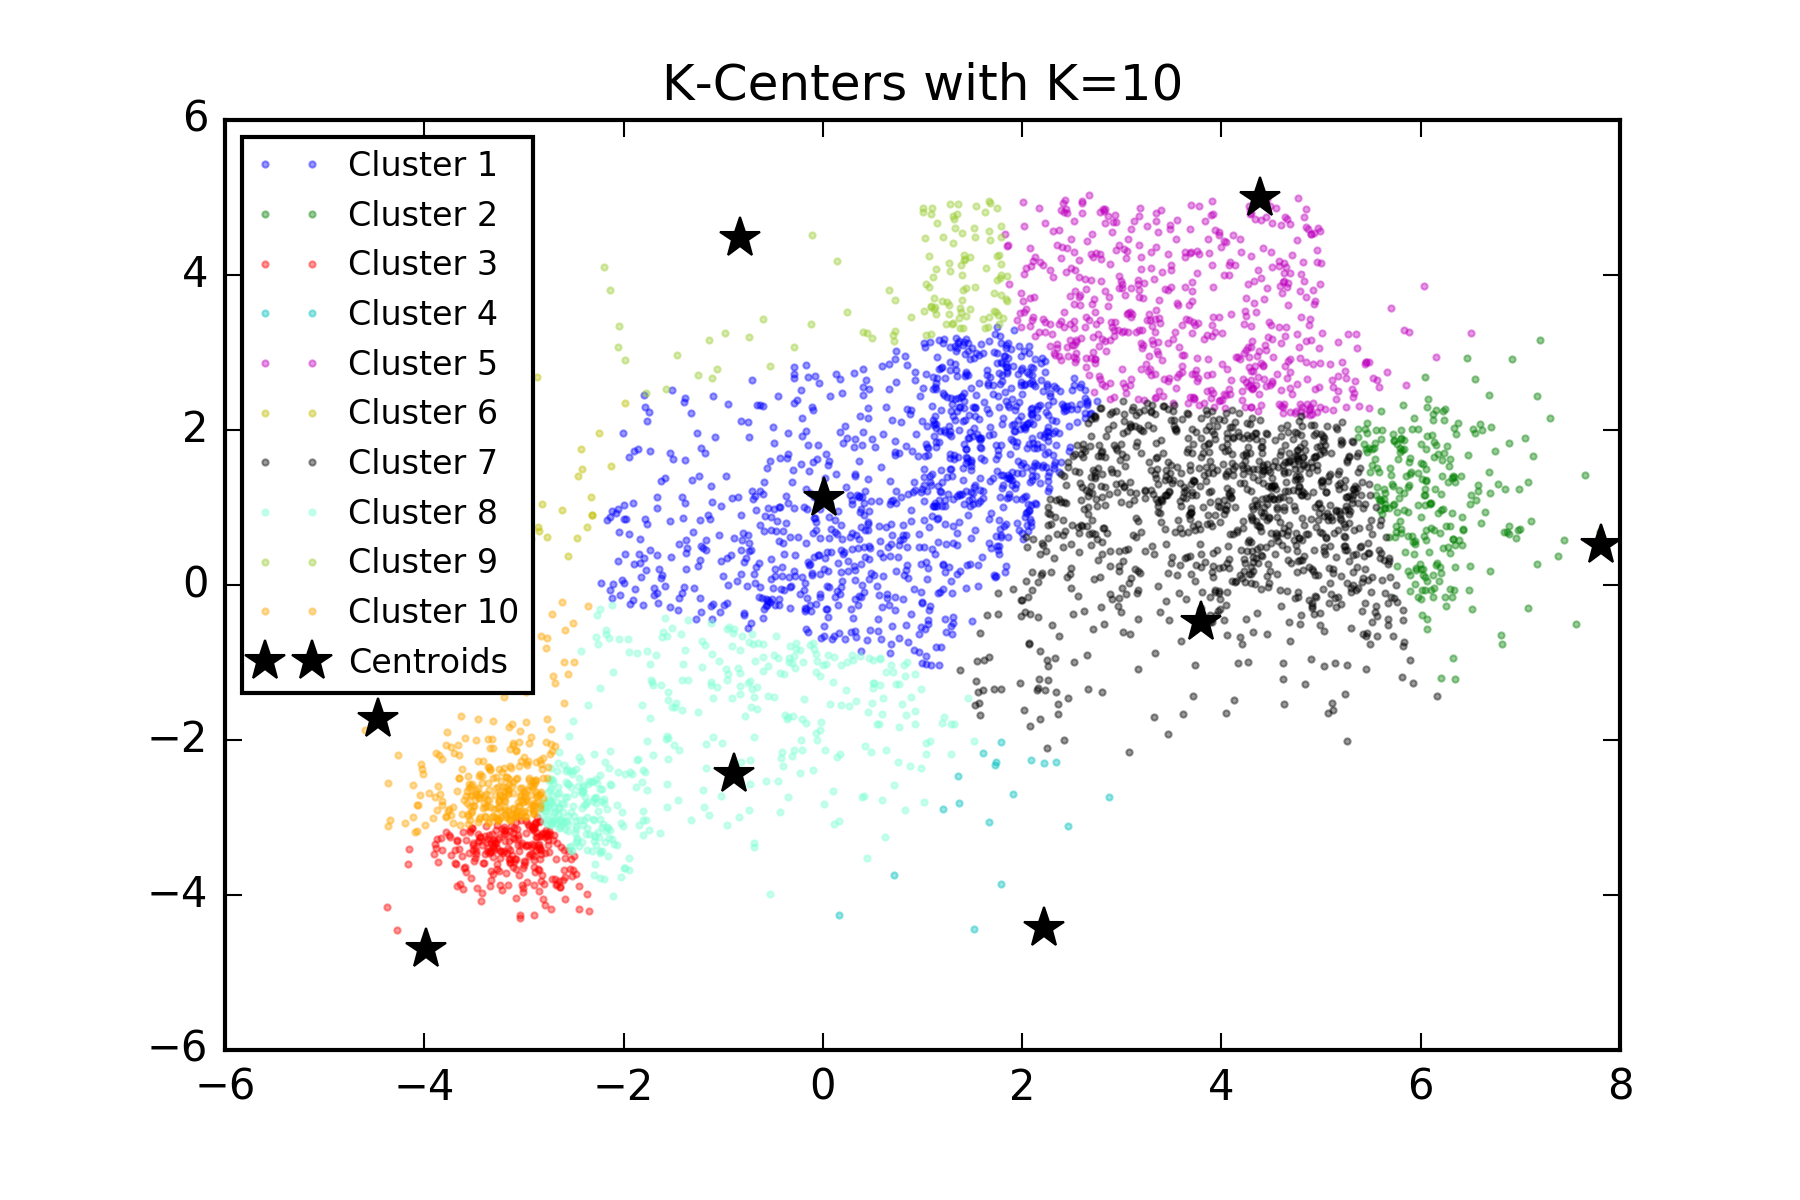
\includegraphics[width=\textwidth]{./figures/bigClustering_kCenter_10.png}
        \end{subfigure}
        
        \caption{Clustering Result for bigClusteringData.txt with K-Center Algorithm}
        \label{fig:kmean_clustering}
\end{figure}

%  -----------------------------------------------------------------------------
\begin{figure}[H]
\centering
\centering
        \begin{subfigure}[b]{0.49\textwidth}
            \centering
            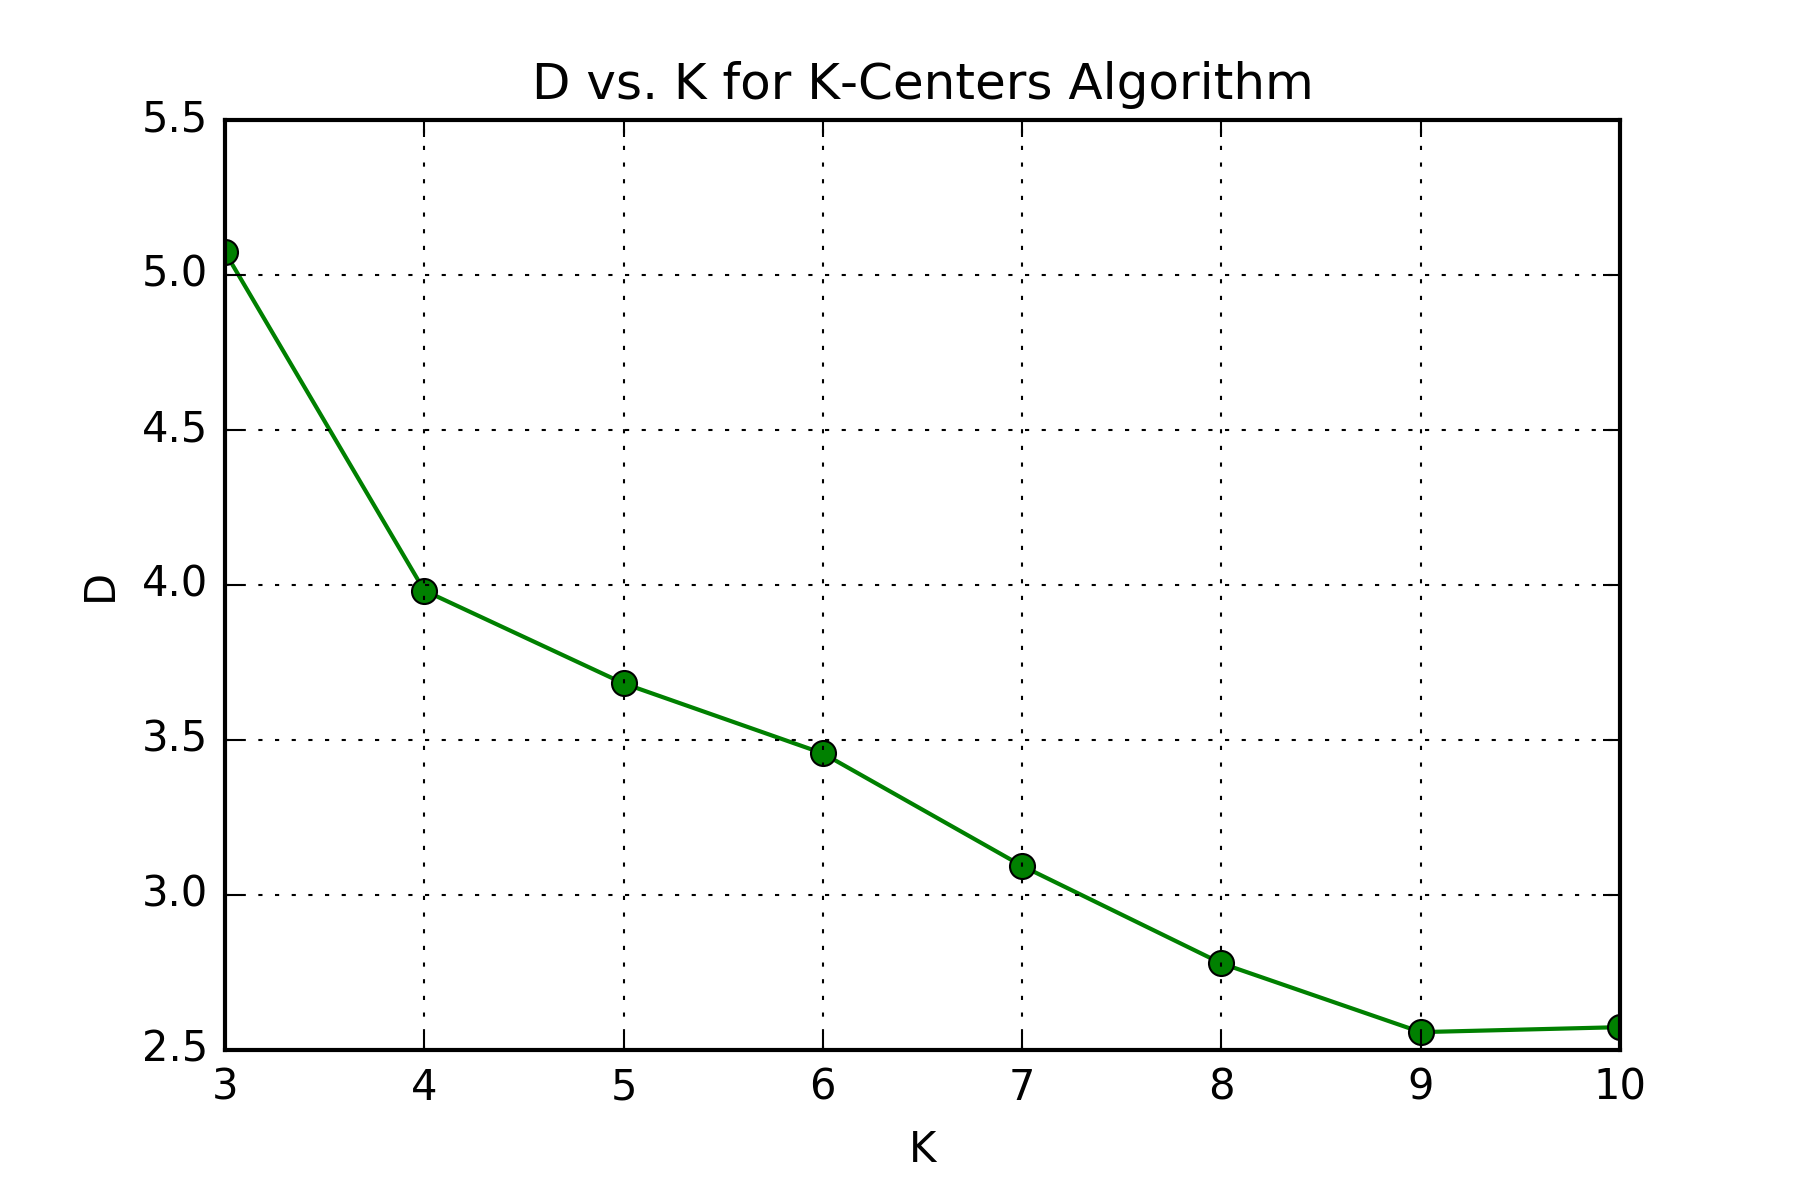
\includegraphics[width=\textwidth]{./figures/loss_clustering_kCenter.png}
            \caption{clustering.txt}\label{fig:6a}
        \end{subfigure}
        \hfill
        \begin{subfigure}[b]{0.49\textwidth}  
            \centering 
            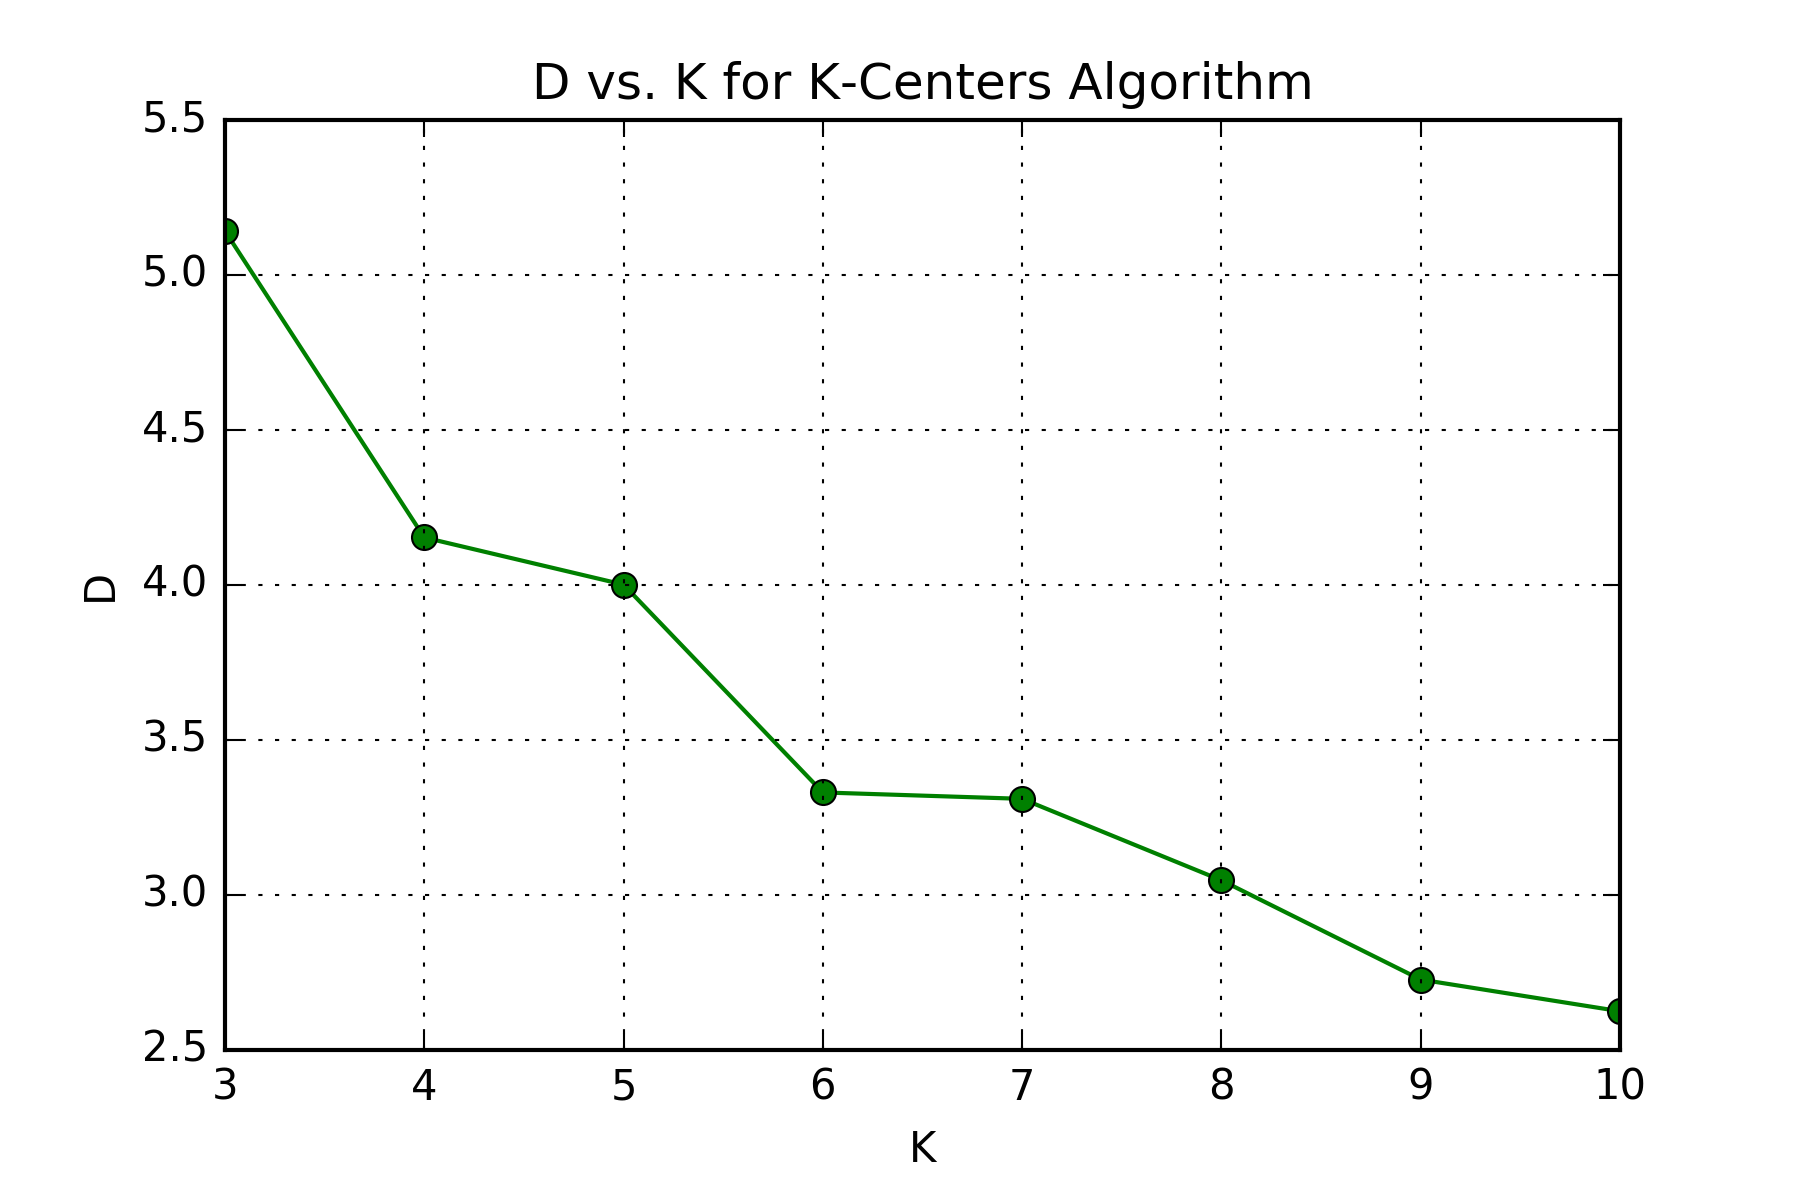
\includegraphics[width=\textwidth]{./figures/loss_bigClustering_kCenter.png}
            \caption{bigClusteringData.txt}\label{fig:6b}
        \end{subfigure}
\caption{Change of Distoration versus Cluster Number K for K-Center Algorithm}
\label{fig:k-means-loss} 
\end{figure}

% -----------------------------------------------------------------------------
\begin{lstlisting}[language=Python, caption=K-Centers Algorithm Python Code]
import numpy as np
import time

def kCenters(X, K, random_state=None, verbose=True):
    """ function to implement the greedy k-centers algorithm """
    np.random.seed(random_state)
    t0 = time.time()

    N, d = X.shape
    # find the initial center
    index = np.random.choice(range(N), size=1)
    Q = np.zeros((K, d))
    Q[0, :] = X[index, :]
    idx = [index]

    i = 1
    while i < K:
        distance = np.zeros((N, i))
        for j in range(i):
            distance[:, j] = np.sum((X - Q[j, :])**2, axis=1)
        min_distance = np.min(distance, axis=1)
        new_index = np.argmax(min_distance)
        idx.append(new_index)
        Q[i, :] = X[new_index, :]
        i += 1

    loss = np.zeros((N, K))
    for i in range(K):
        loss[:, i] = np.sqrt(np.sum((X - Q[i, :])**2, axis=1))
    D = np.max(np.min(loss, axis=1))
    C = np.argmin(loss, axis=1)

    if verbose is True:
        t = np.round(time.time() - t0, 4)
        print('K-Centers is finished in ' + str(t) + 's')

    return Q, C, D, idx
\end{lstlisting}

% -----------------------------------------------------------------------------
\section*{\Large \Romannum{3}. Single-Swap Algorithm}

%  -----------------------------------------------------------------------------
\begin{figure}[htb]
        \centering
        \begin{subfigure}[b]{0.475\textwidth}
            \centering
            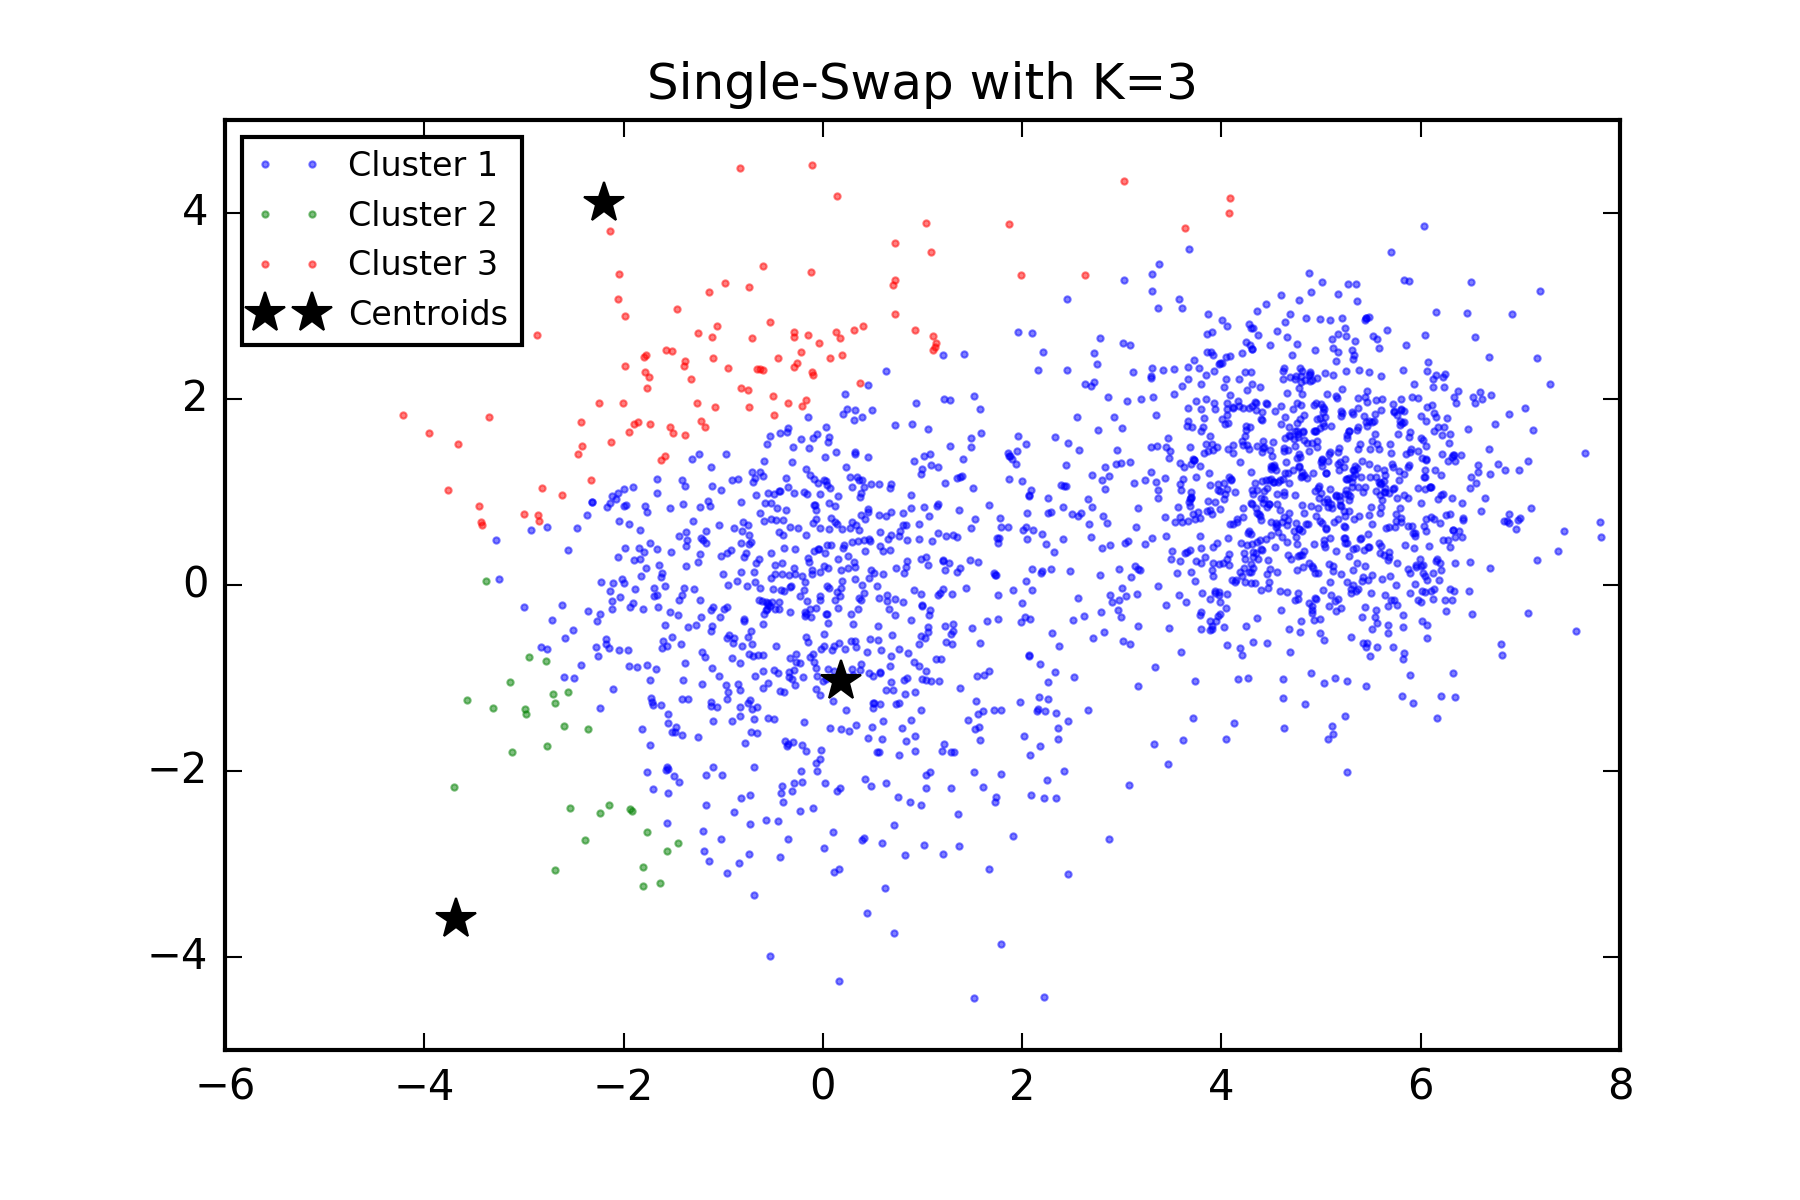
\includegraphics[width=\textwidth]{./figures/clustering_singleSwap_3.png}
        \end{subfigure}
        \hfill
        \begin{subfigure}[b]{0.475\textwidth}  
            \centering 
            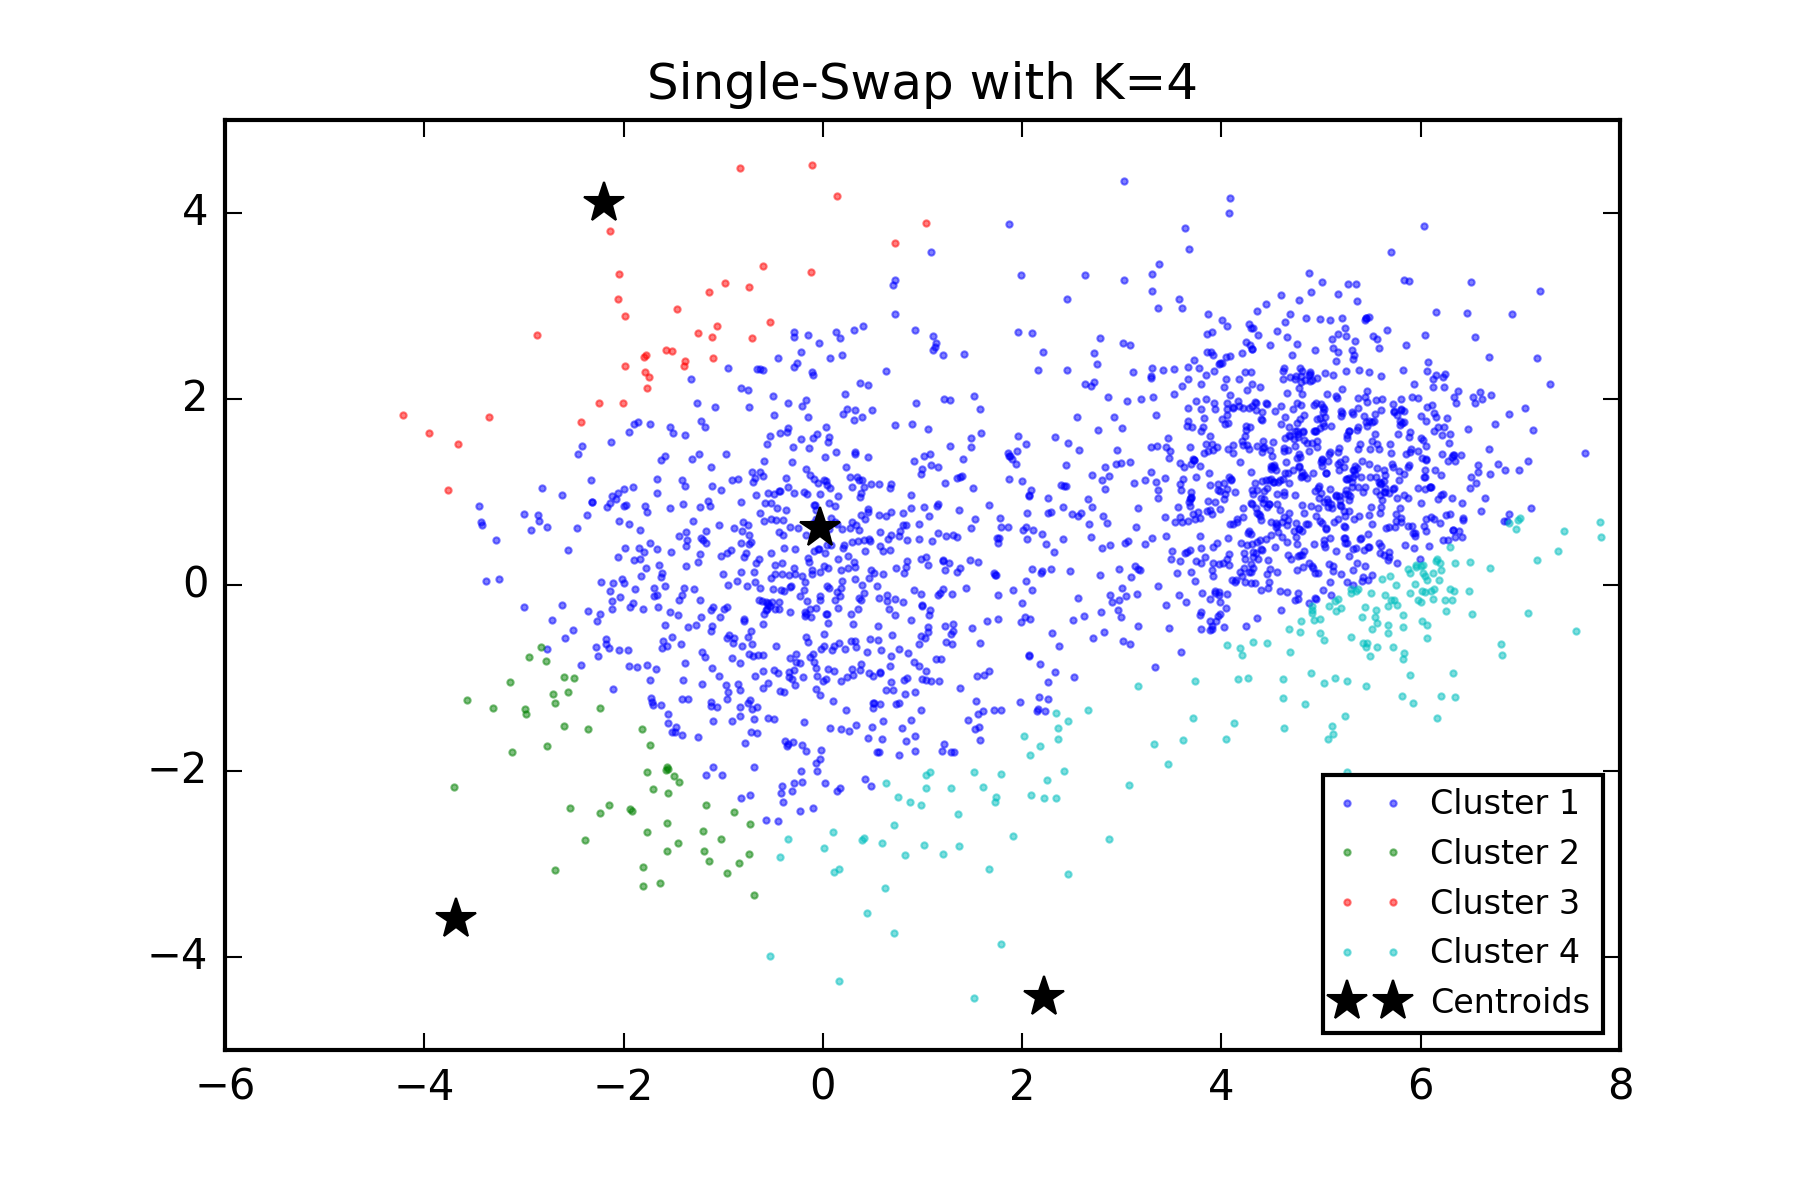
\includegraphics[width=\textwidth]{./figures/clustering_singleSwap_4.png}
        \end{subfigure}
%        \vskip\baselineskip        
        \begin{subfigure}[b]{0.475\textwidth}  
            \centering 
            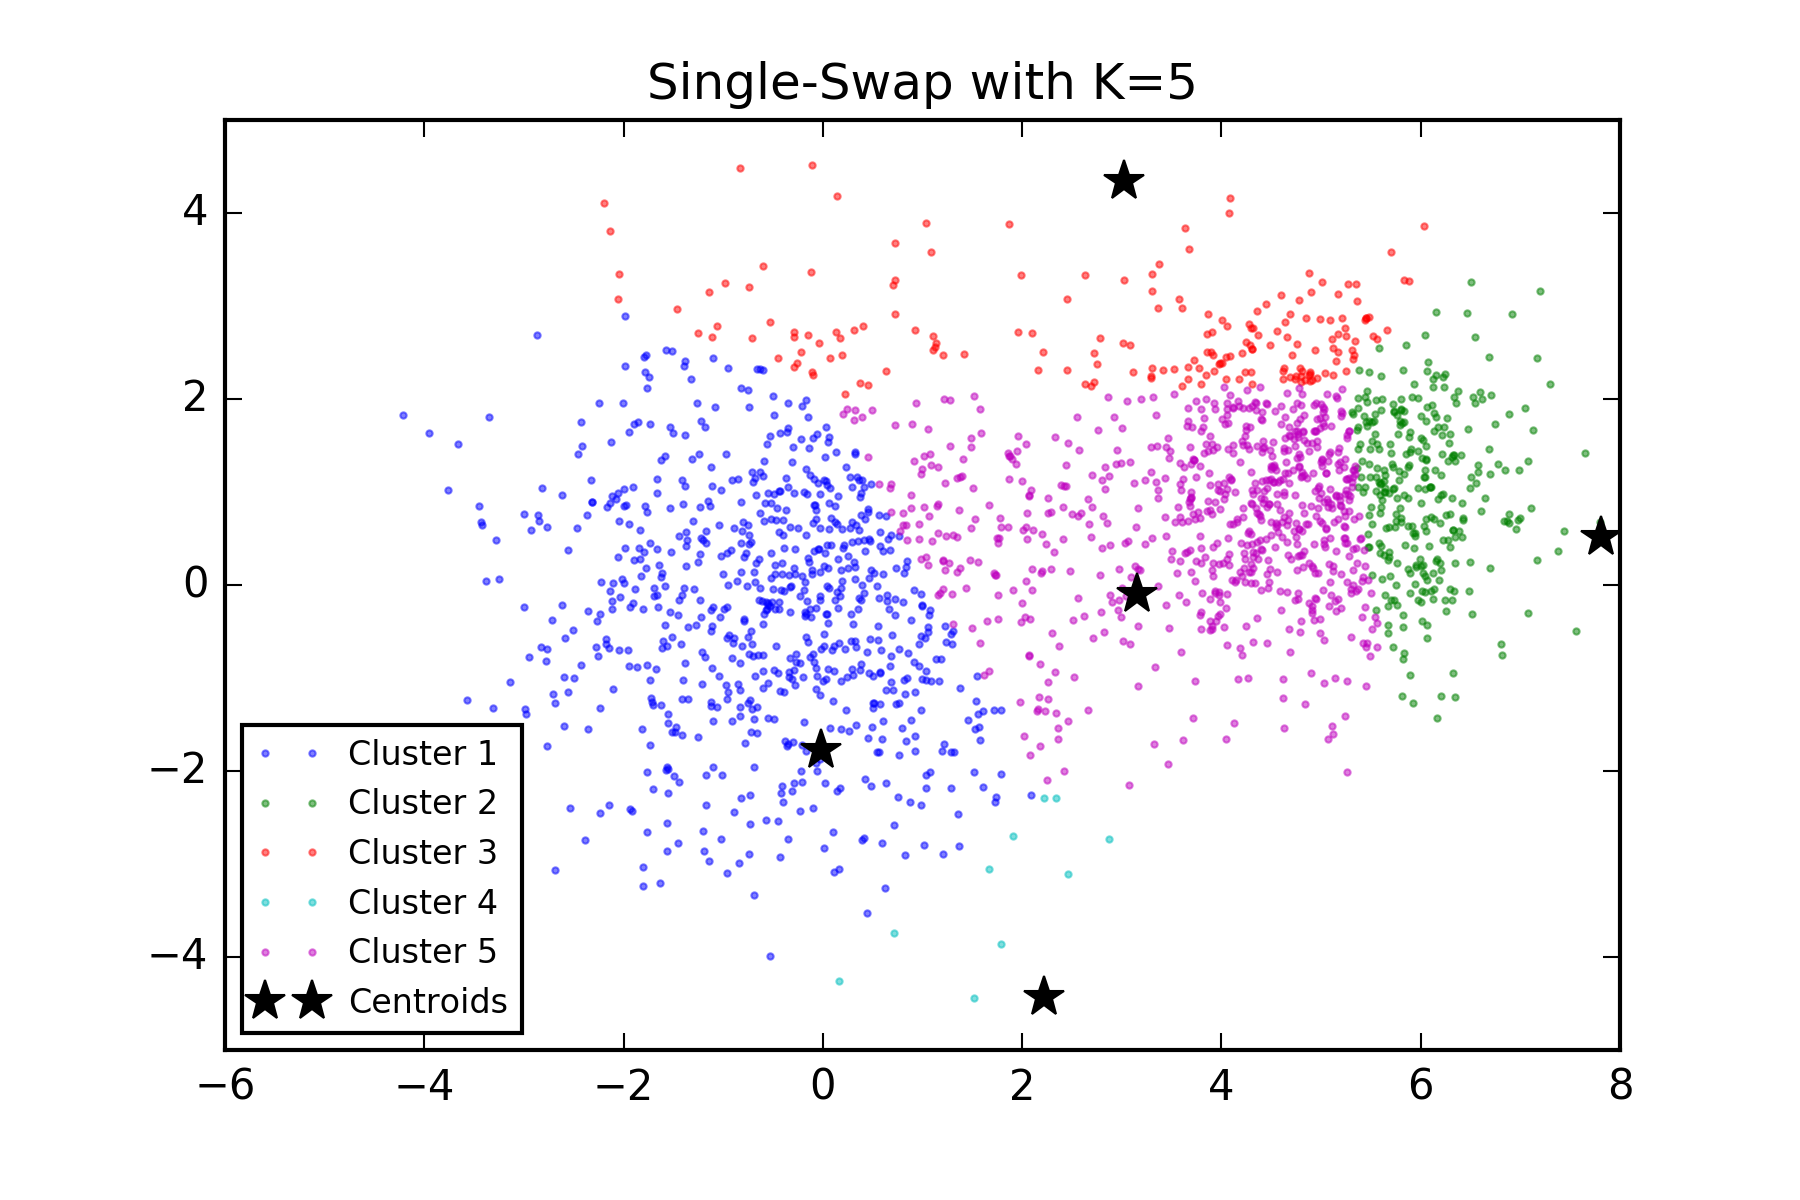
\includegraphics[width=\textwidth]{./figures/clustering_singleSwap_5.png}
        \end{subfigure}
        \hfill
        \begin{subfigure}[b]{0.475\textwidth}   
            \centering 
            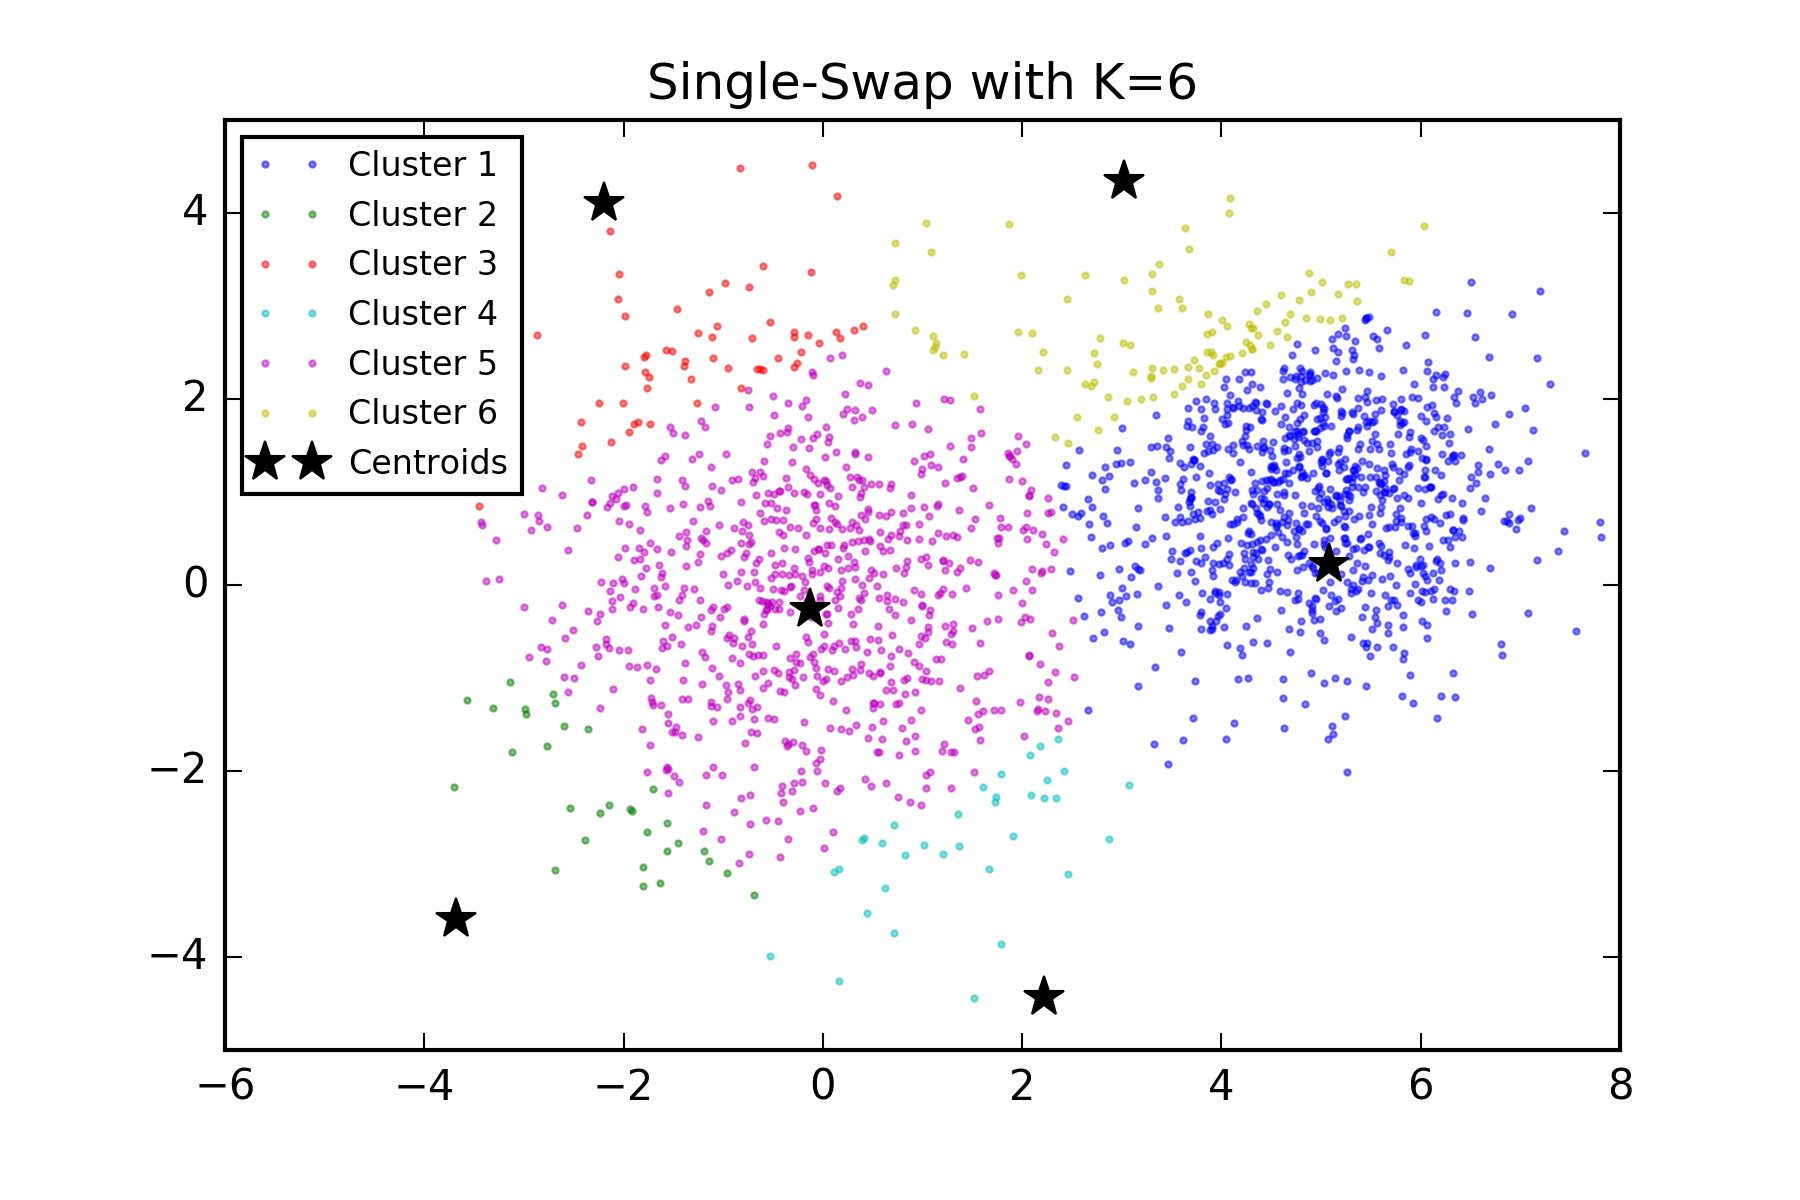
\includegraphics[width=\textwidth]{./figures/clustering_singleSwap_6.png}
        \end{subfigure}
%        \vskip\baselineskip     
        \begin{subfigure}[b]{0.475\textwidth}   
            \centering 
            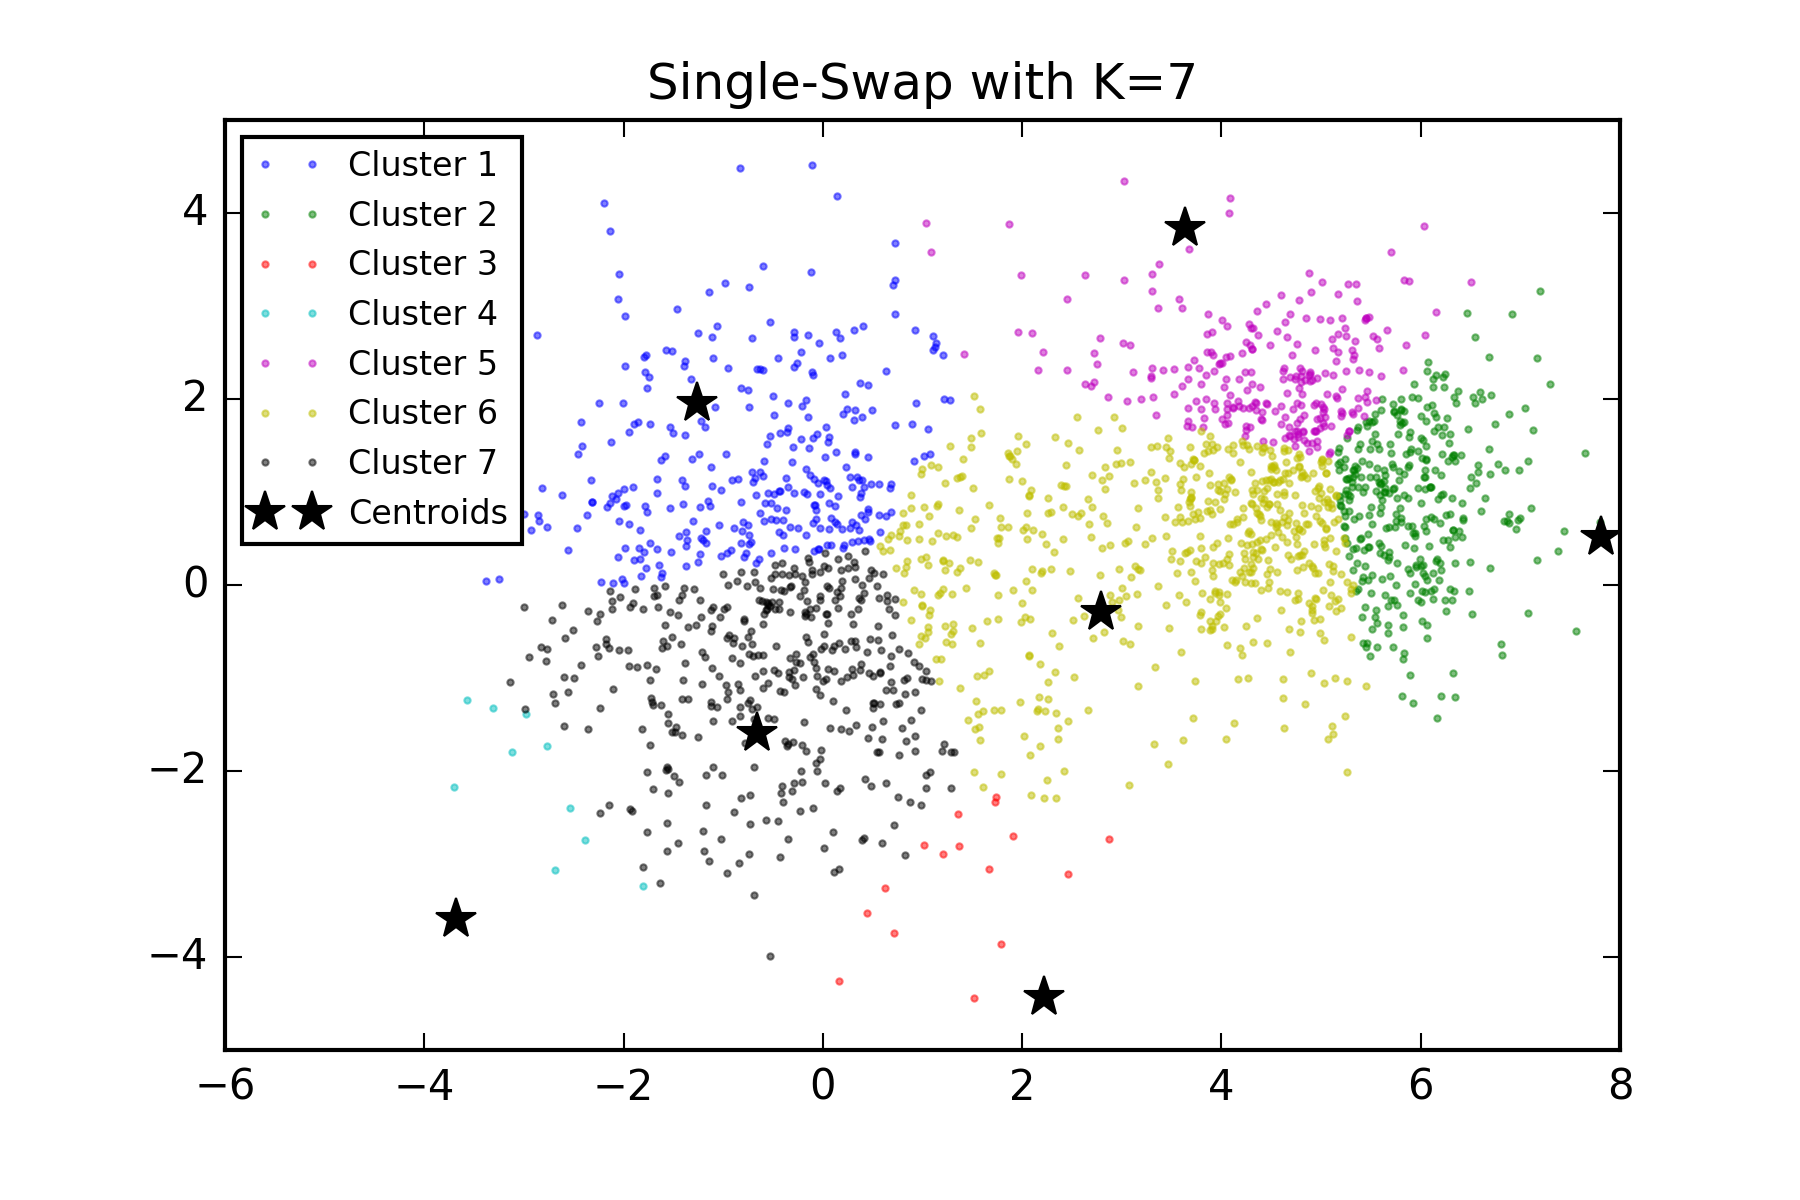
\includegraphics[width=\textwidth]{./figures/clustering_singleSwap_7.png}
        \end{subfigure}
        \hfill
        \begin{subfigure}[b]{0.475\textwidth}  
            \centering 
            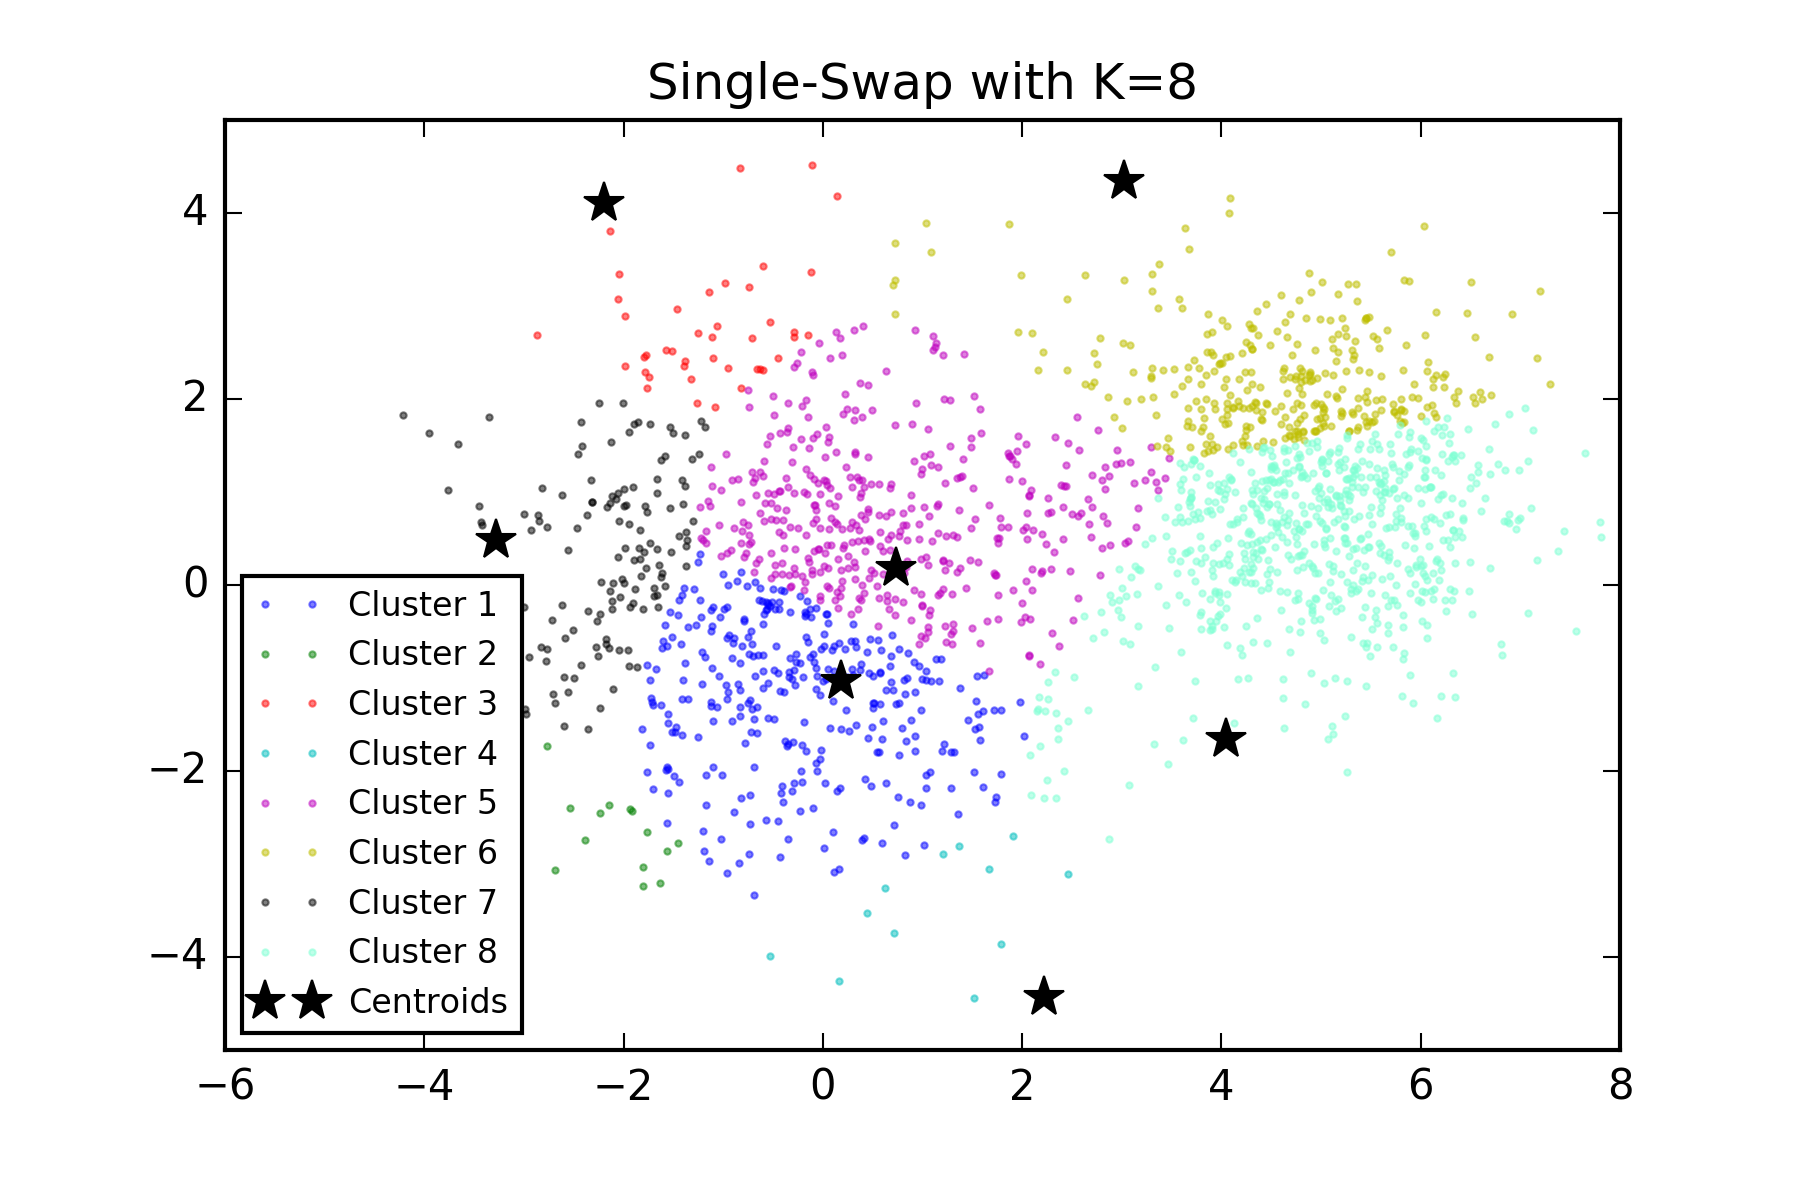
\includegraphics[width=\textwidth]{./figures/clustering_singleSwap_8.png}
        \end{subfigure}
%        \vskip\baselineskip
        \begin{subfigure}[b]{0.475\textwidth}   
            \centering 
            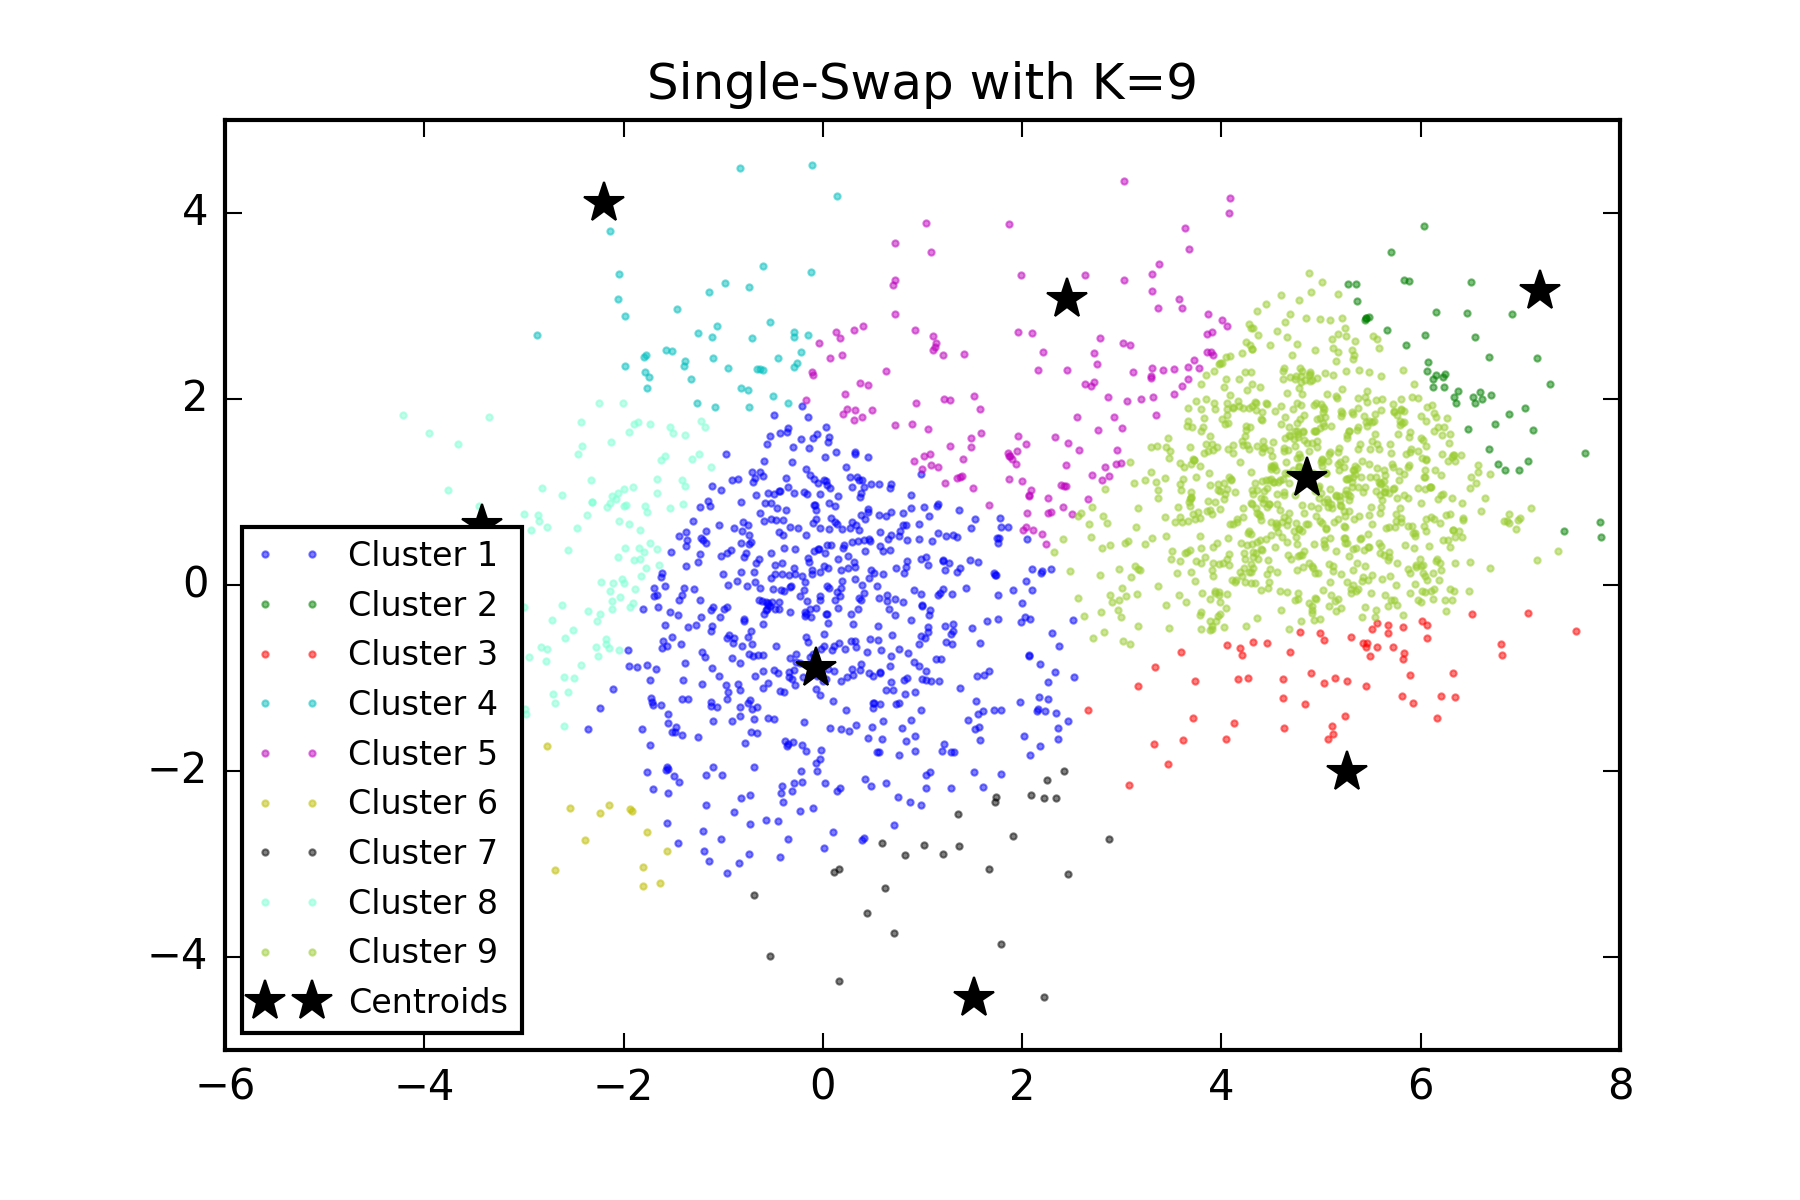
\includegraphics[width=\textwidth]{./figures/clustering_singleSwap_9.png}
        \end{subfigure}
        \hfill
        \begin{subfigure}[b]{0.475\textwidth}   
            \centering 
            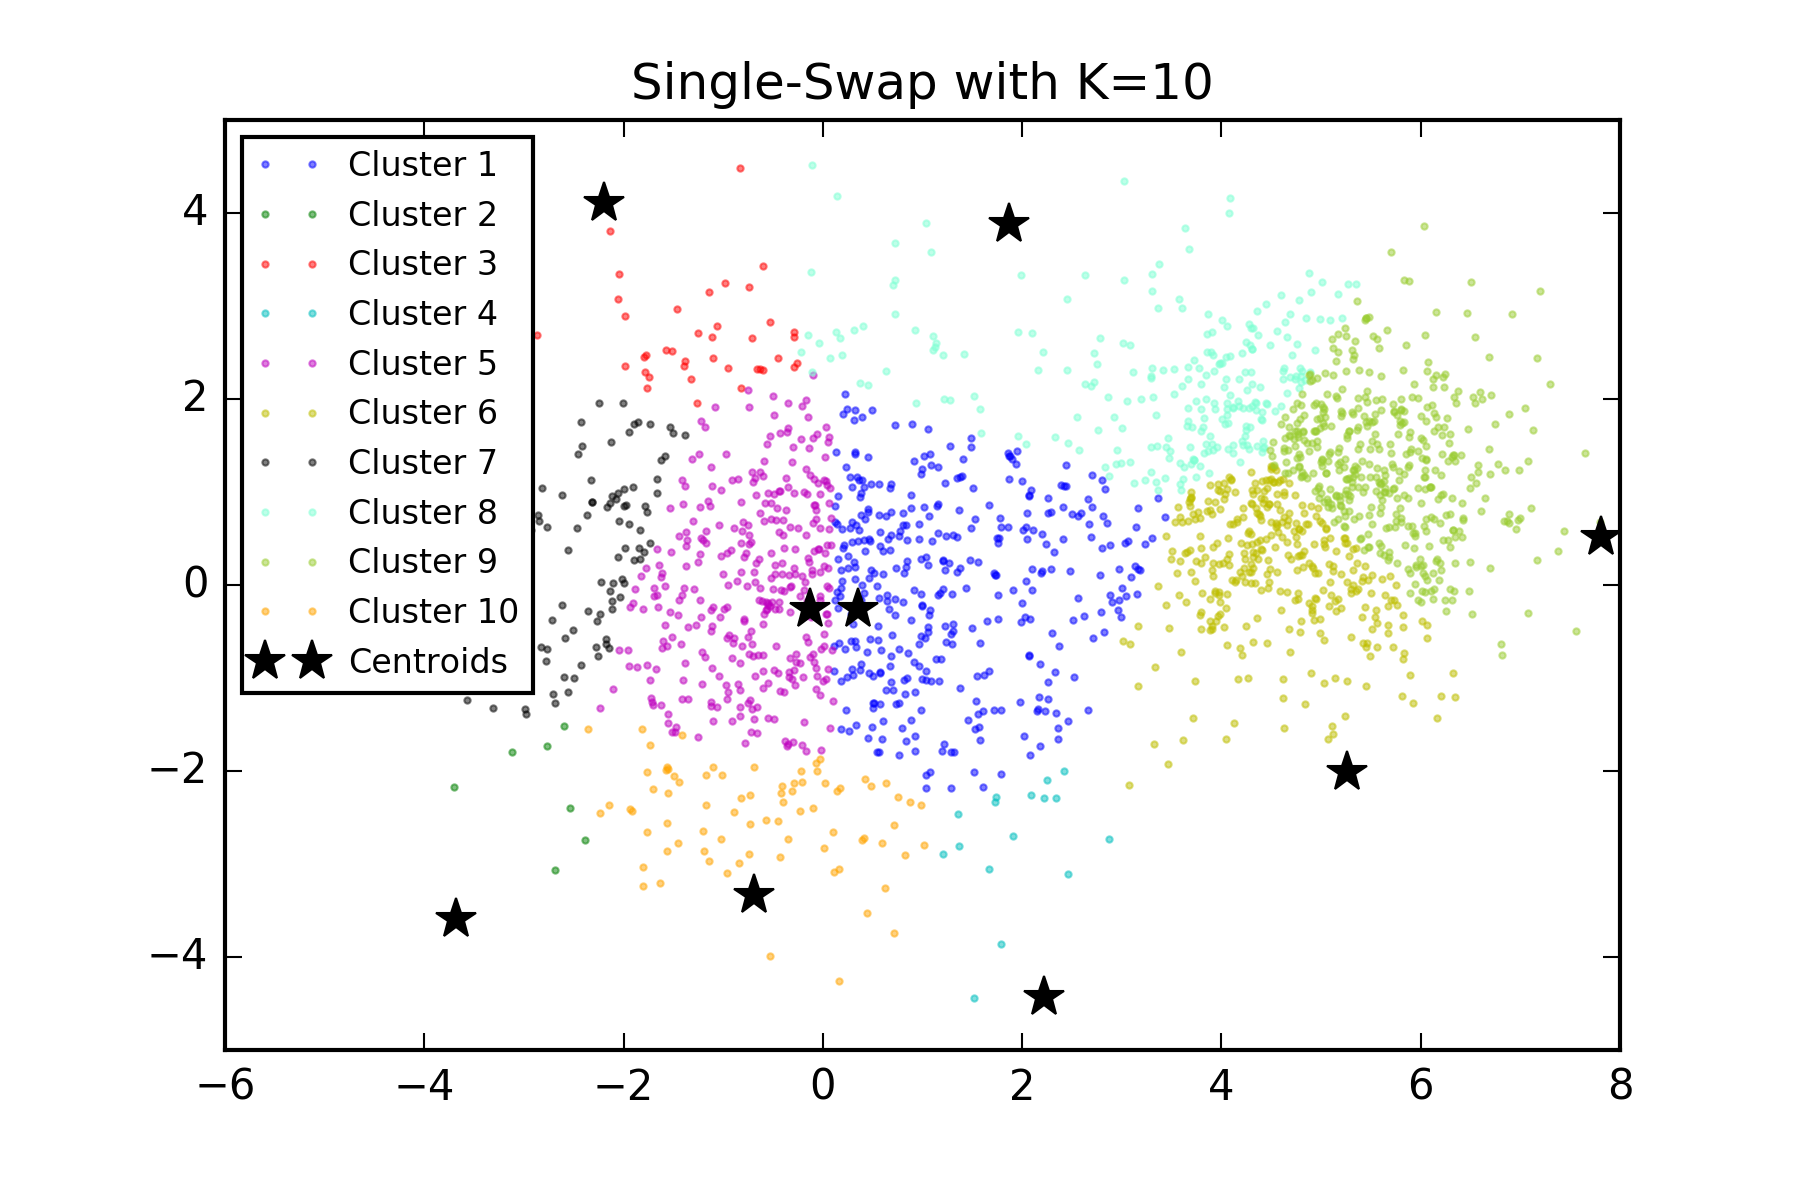
\includegraphics[width=\textwidth]{./figures/clustering_singleSwap_10.png}
        \end{subfigure}
        
        \caption{Clustering Result for clustering.txt with Single-Swap Algorithm}
        \label{fig:kmean_clustering}
\end{figure}

%  -----------------------------------------------------------------------------
\begin{figure}[htb]
        \centering
        \begin{subfigure}[b]{0.475\textwidth}
            \centering
            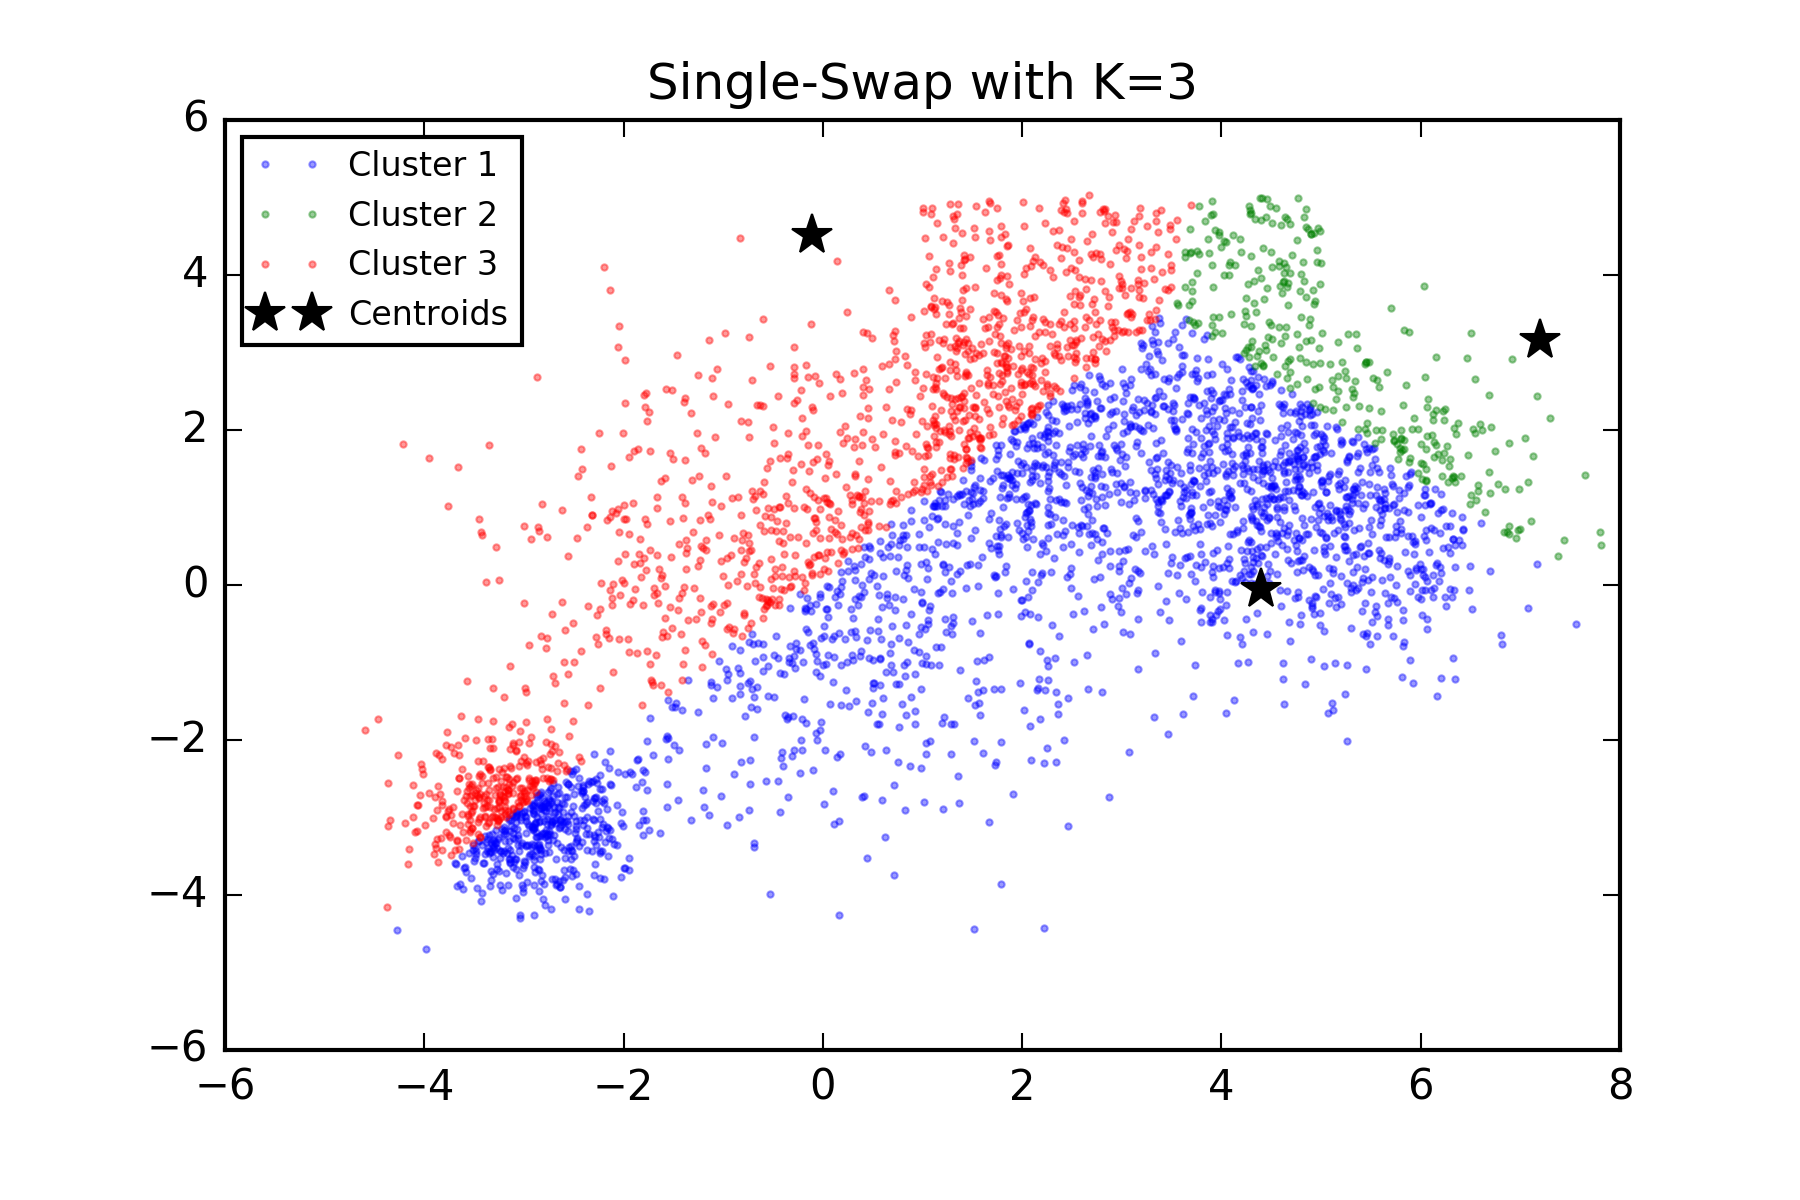
\includegraphics[width=\textwidth]{./figures/bigClustering_singleSwap_3.png}
        \end{subfigure}
        \hfill
        \begin{subfigure}[b]{0.475\textwidth}  
            \centering 
            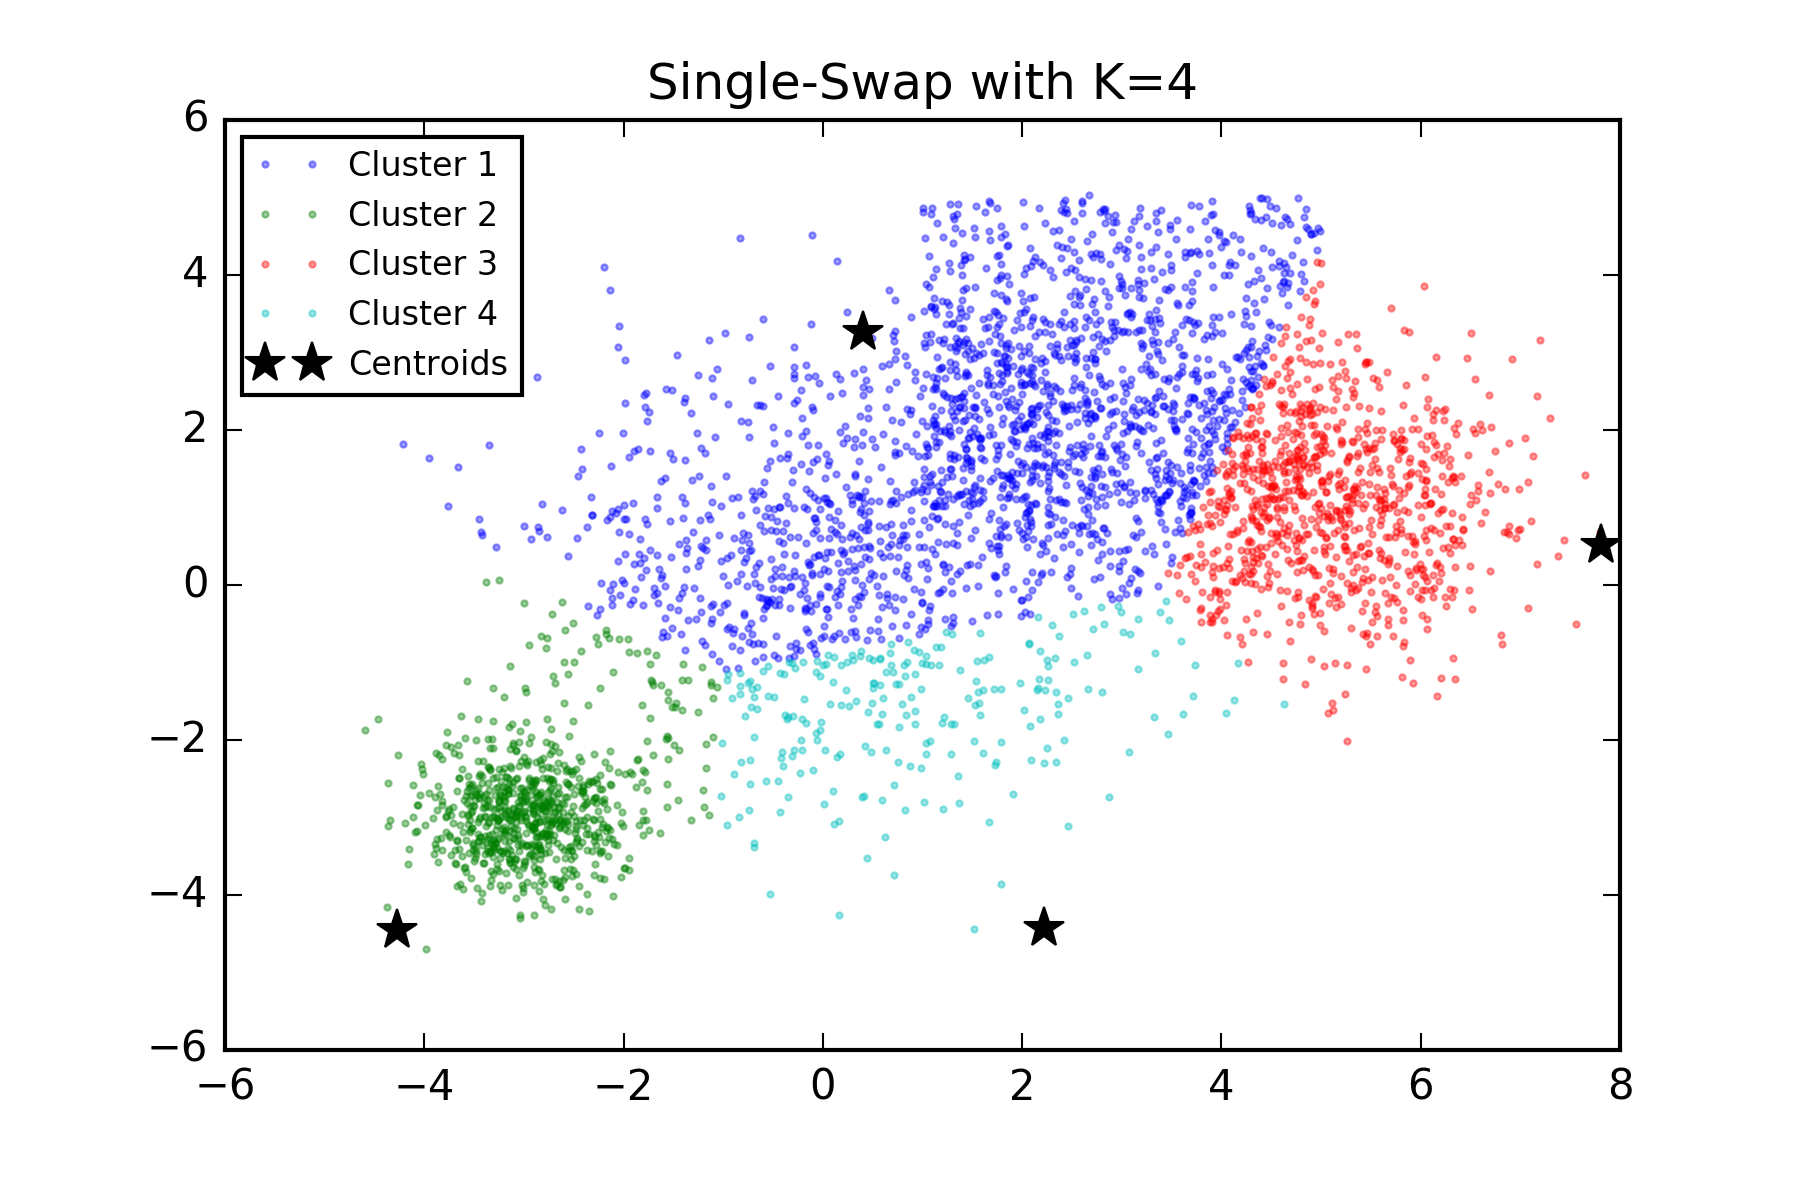
\includegraphics[width=\textwidth]{./figures/bigClustering_singleSwap_4.png}
        \end{subfigure}
%        \vskip\baselineskip        
        \begin{subfigure}[b]{0.475\textwidth}  
            \centering 
            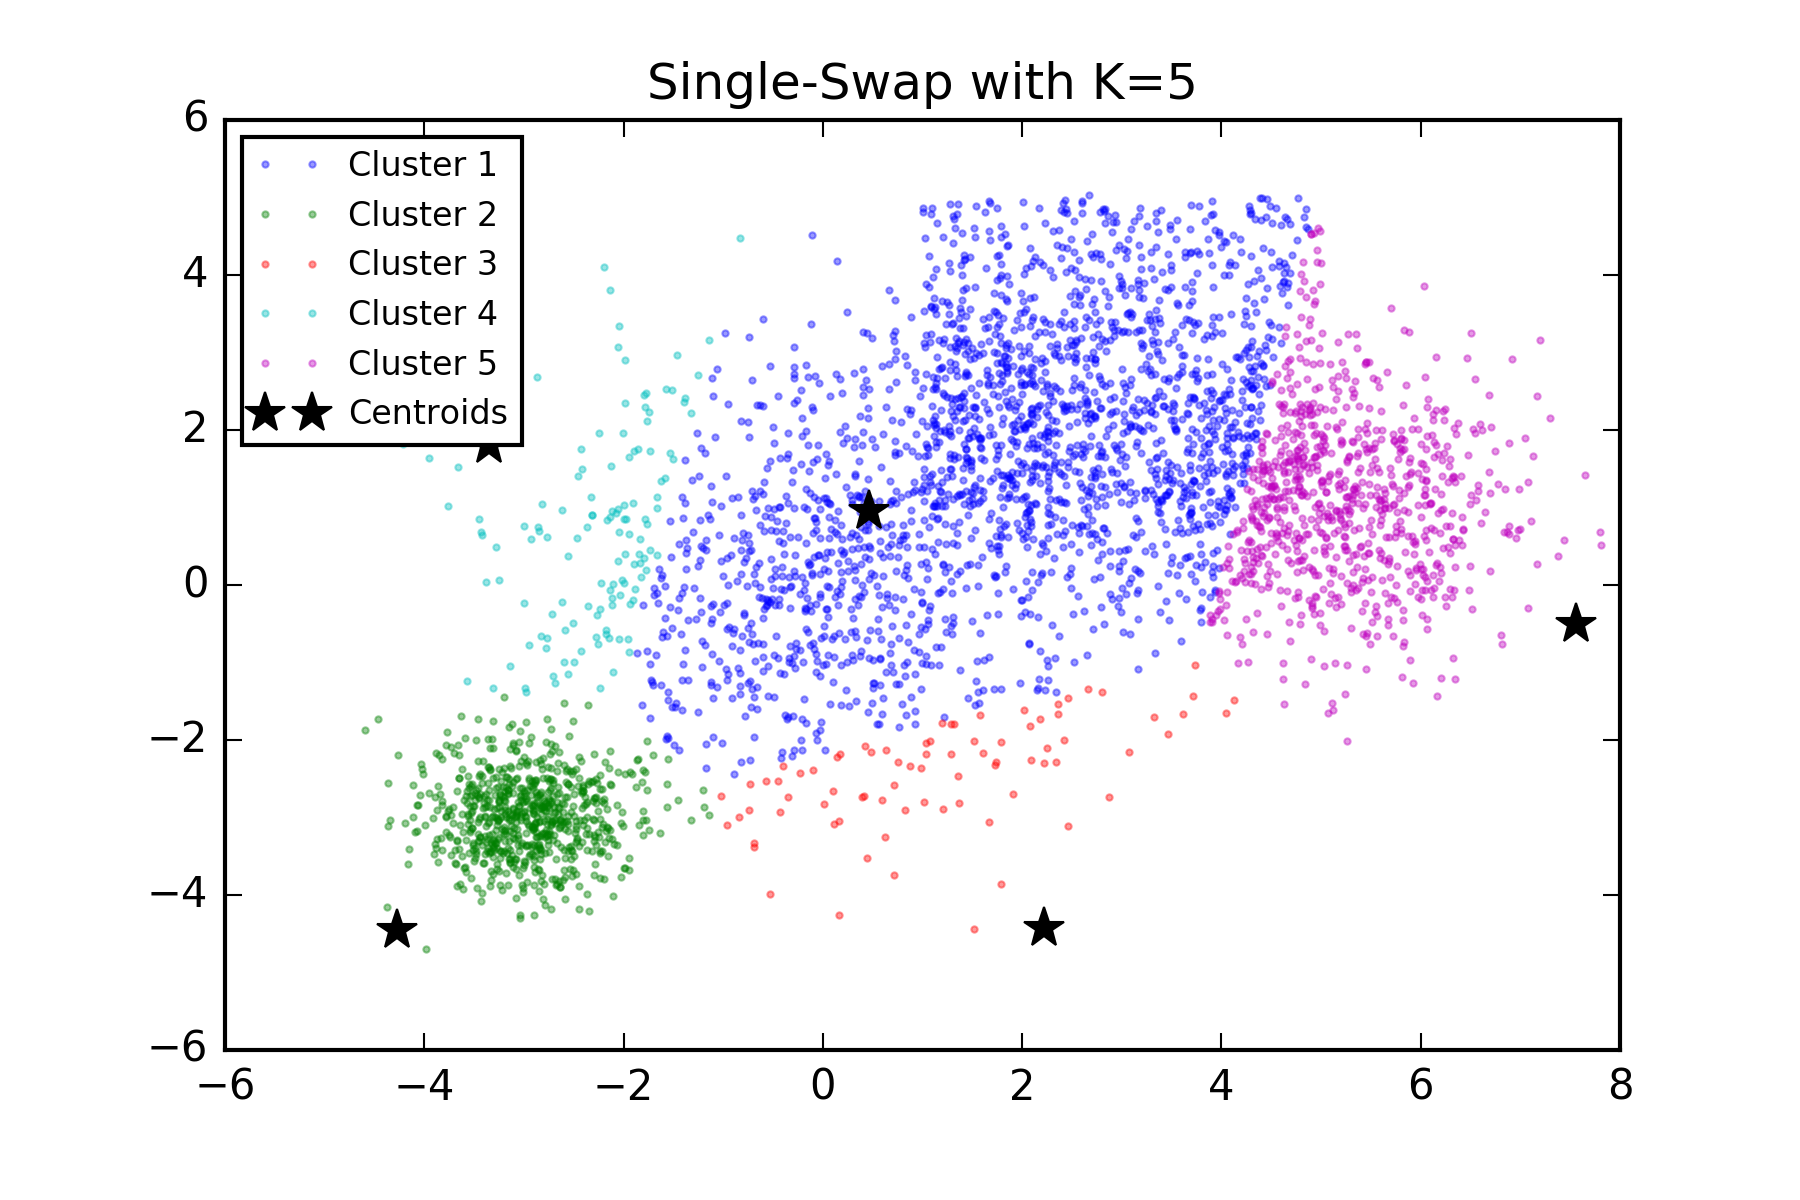
\includegraphics[width=\textwidth]{./figures/bigClustering_singleSwap_5.png}
        \end{subfigure}
        \hfill
        \begin{subfigure}[b]{0.475\textwidth}   
            \centering 
            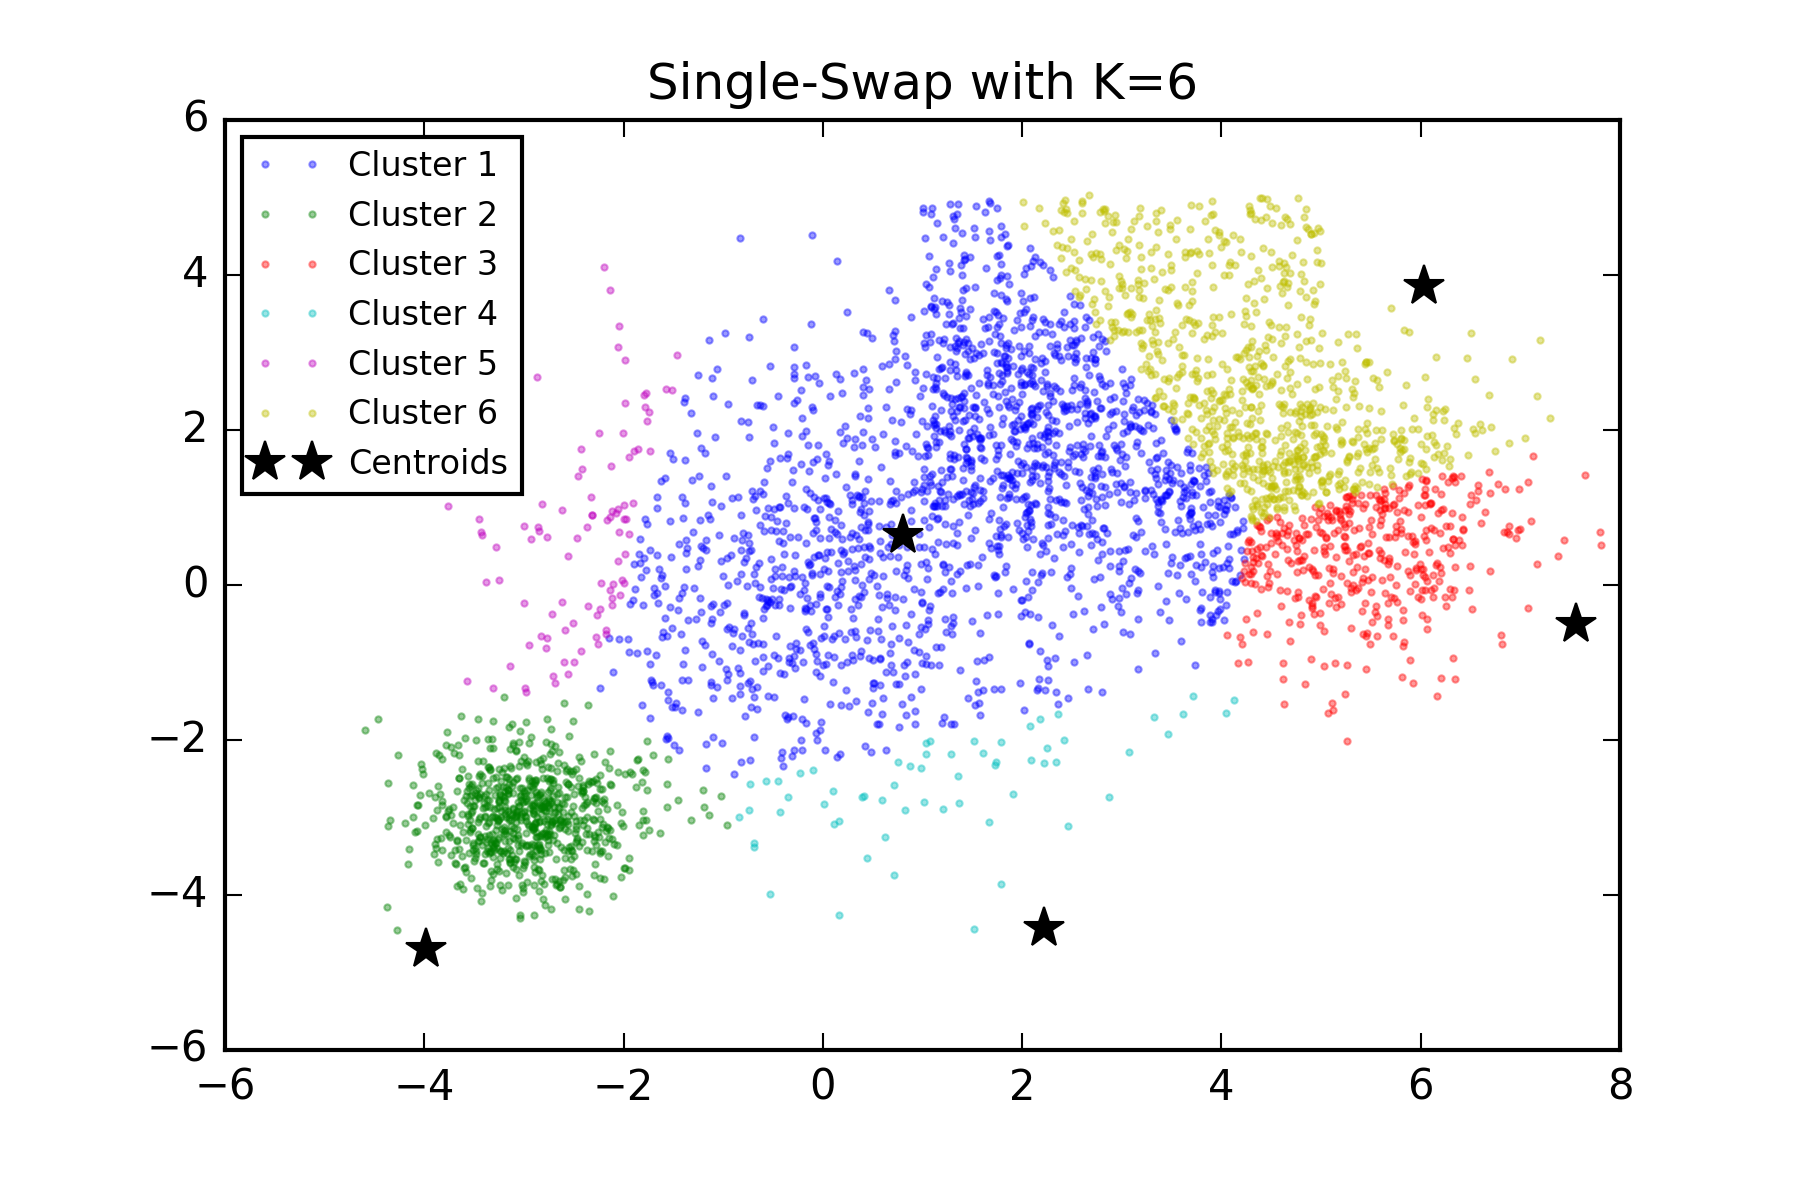
\includegraphics[width=\textwidth]{./figures/bigClustering_singleSwap_6.png}
        \end{subfigure}
%        \vskip\baselineskip     
        \begin{subfigure}[b]{0.475\textwidth}   
            \centering 
            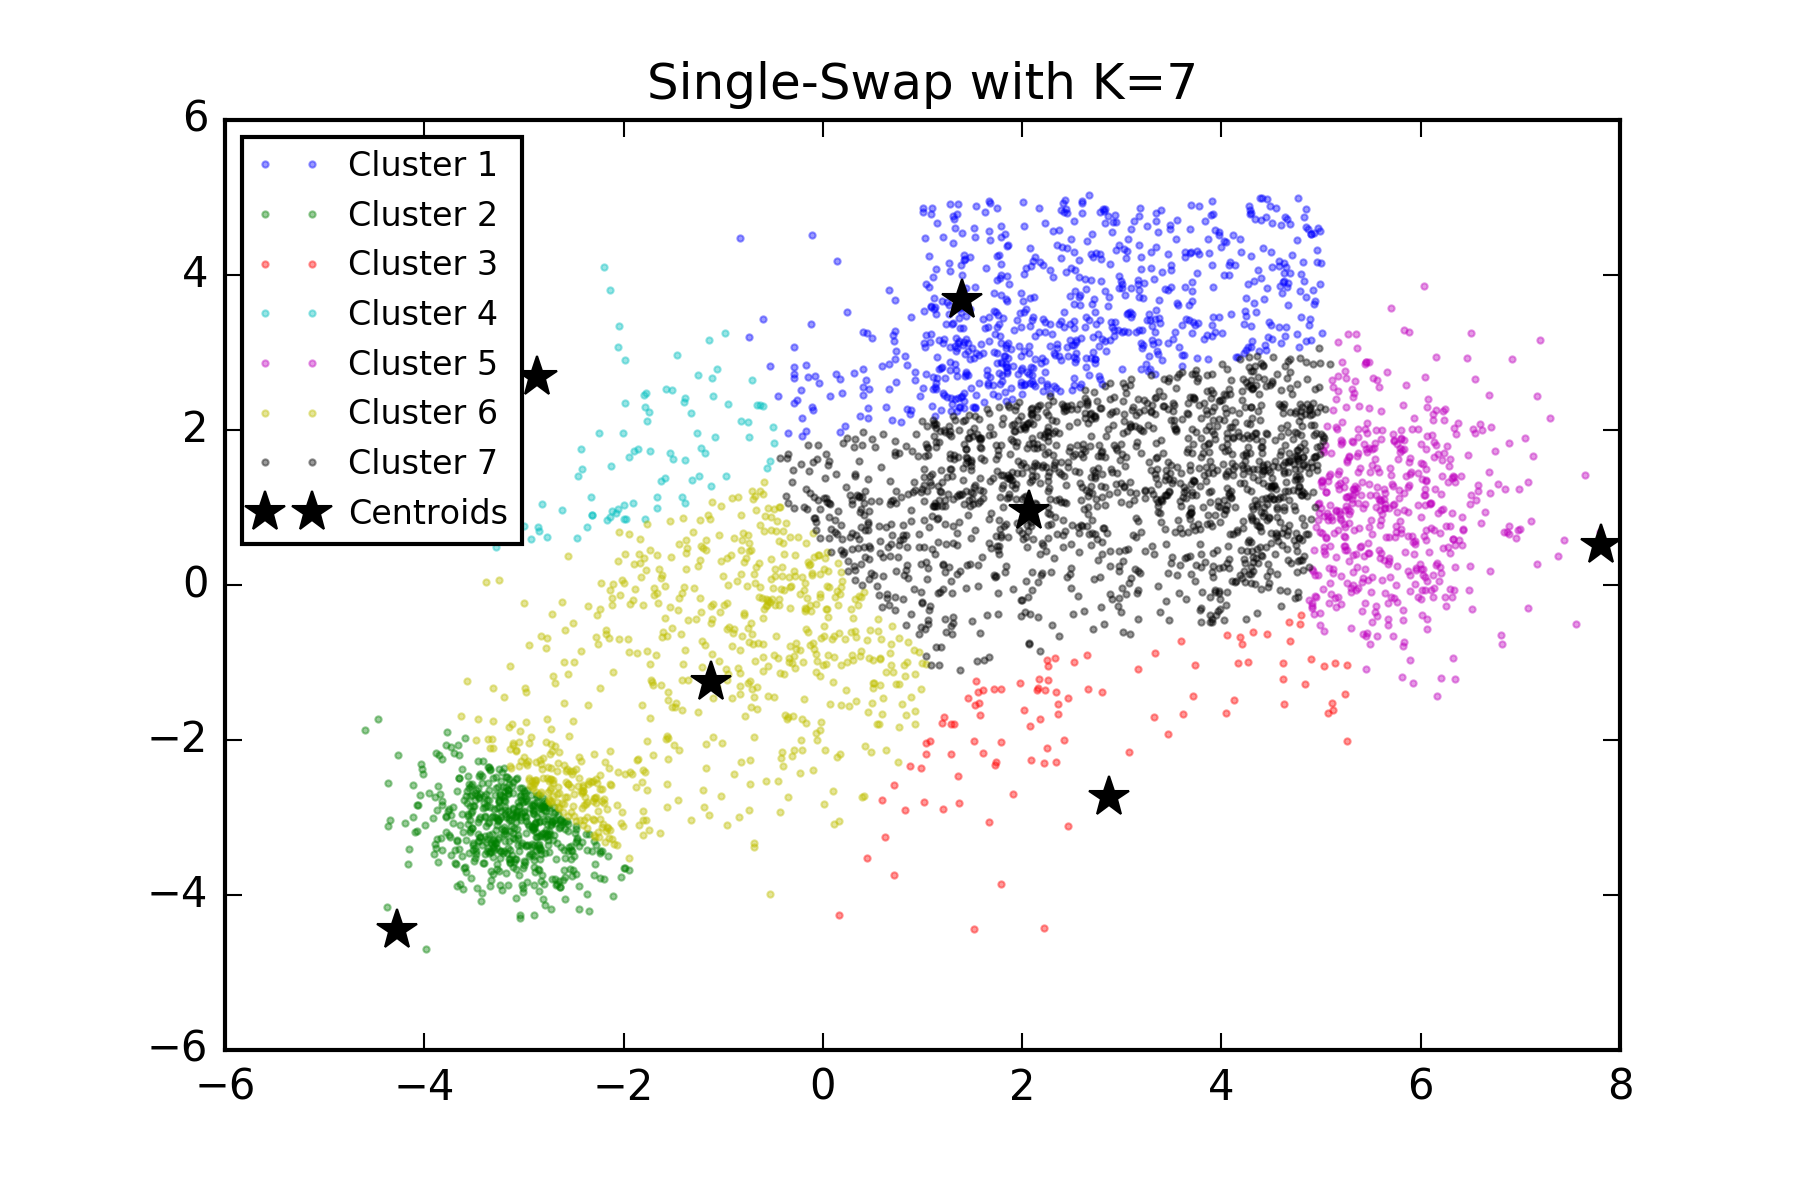
\includegraphics[width=\textwidth]{./figures/bigClustering_singleSwap_7.png}
        \end{subfigure}
        \hfill
        \begin{subfigure}[b]{0.475\textwidth}  
            \centering 
            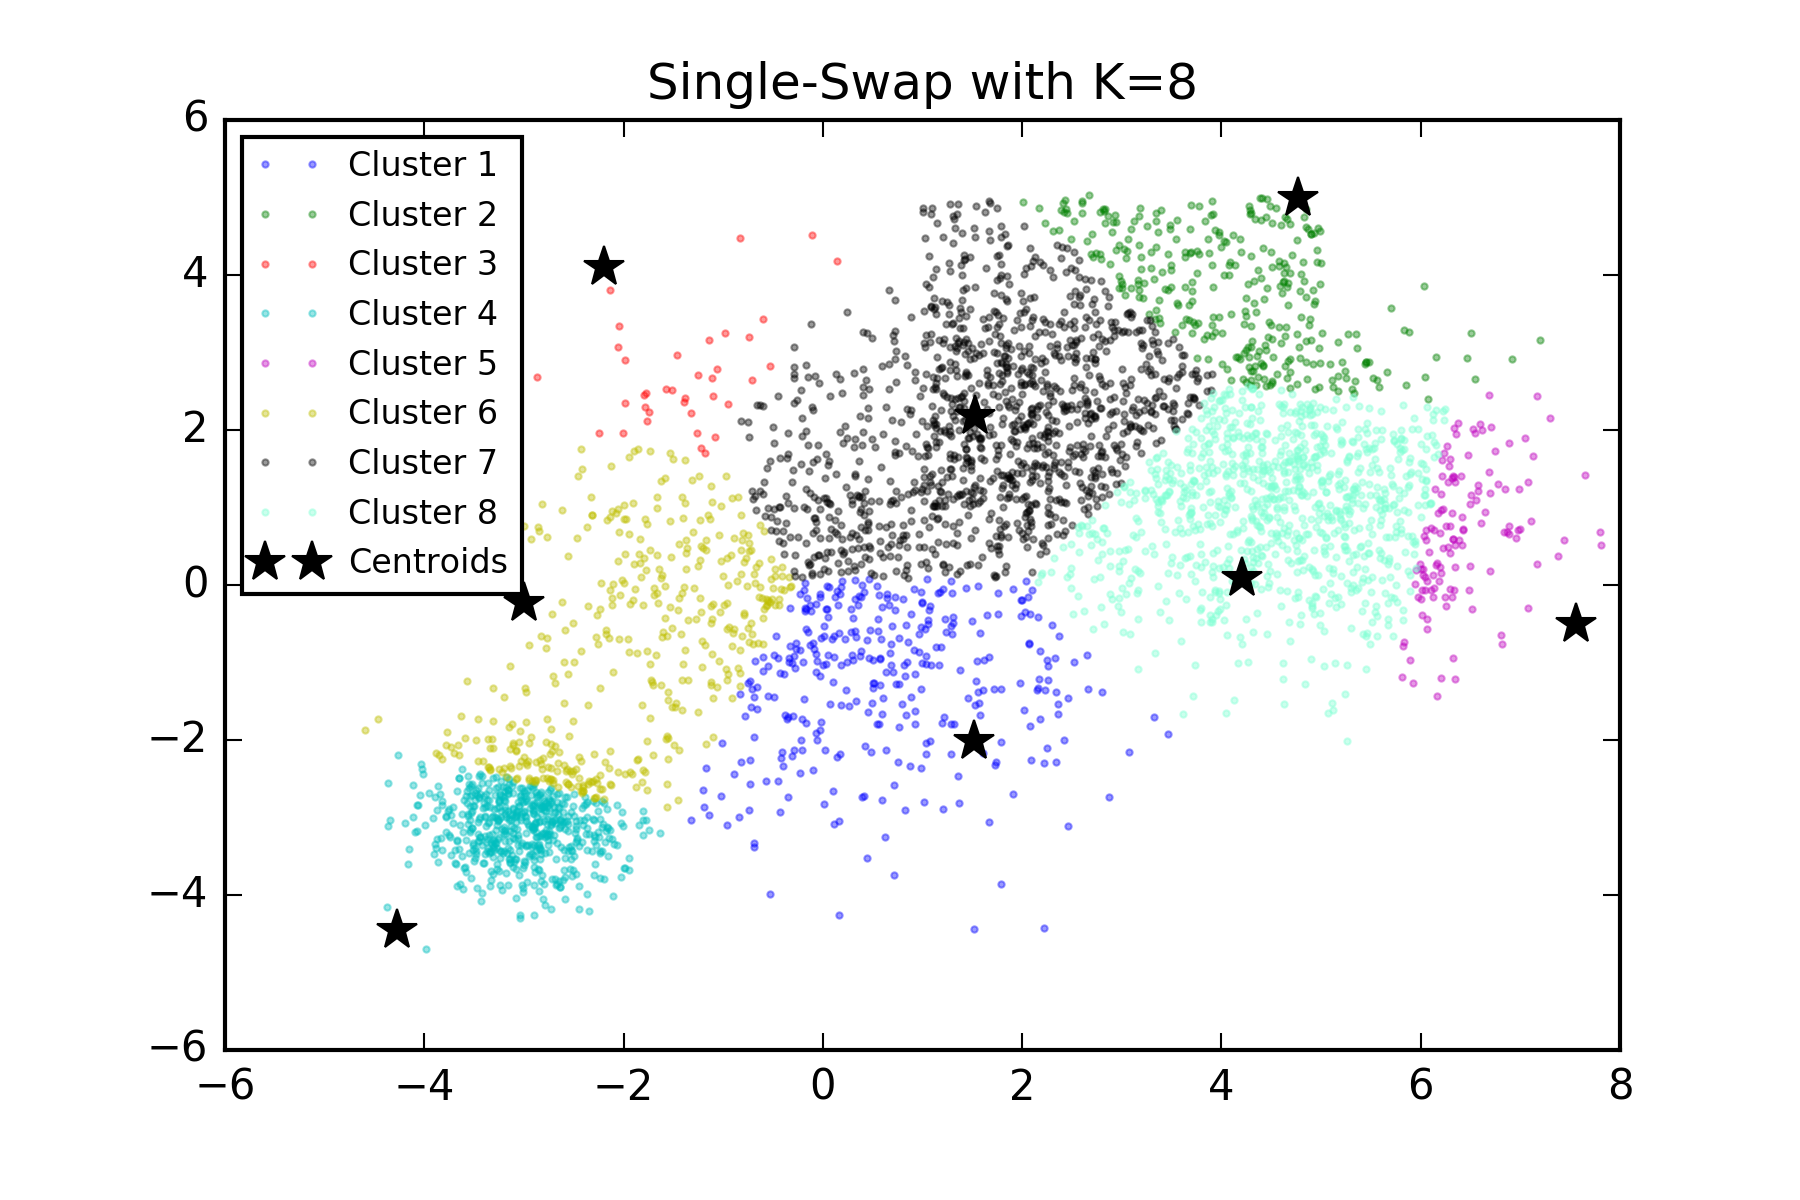
\includegraphics[width=\textwidth]{./figures/bigClustering_singleSwap_8.png}
        \end{subfigure}
%        \vskip\baselineskip
        \begin{subfigure}[b]{0.475\textwidth}   
            \centering 
            \includegraphics[width=\textwidth]{./figures/bigClustering_singleSwap_9.png}
        \end{subfigure}
        \hfill
        \begin{subfigure}[b]{0.475\textwidth}   
            \centering 
            \includegraphics[width=\textwidth]{./figures/bigClustering_singleSwap_10.png}
        \end{subfigure}
        
        \caption{Clustering Result for bigClusteringData.txt with Single-Swap Algorithm}
        \label{fig:kmean_clustering}
\end{figure}

%  -----------------------------------------------------------------------------
\begin{figure}[H]
\centering
\centering
        \begin{subfigure}[b]{0.49\textwidth}
            \centering
            \includegraphics[width=\textwidth]{./figures/loss_clustering_singleSwap.png}
            \caption{clustering.txt}\label{fig:9a}
        \end{subfigure}
        \hfill
        \begin{subfigure}[b]{0.49\textwidth}  
            \centering 
            \includegraphics[width=\textwidth]{./figures/loss_bigClustering_singleSwap.png}
            \caption{bigClusteringData.txt}\label{fig:9b}
        \end{subfigure}
\caption{Change of Distoration versus Cluster Number K for Single-Swap Algorithm}
\label{fig:k-means-loss} 
\end{figure}

% -----------------------------------------------------------------------------
\begin{lstlisting}[language=Python, caption=Single-Swap Algorithm Python Code]
import numpy as np
import time
from k_centers import kCenters

def singleSwap(X, K, tau=0.05, random_state=None, verbose=True):
    """ function to implement the single-swap for k-centers algorithm """
    t0 = time.time()

    # calculate the initial centers
    Q, _, pre_cost, _ = kCenters(X, K, random_state=random_state,
                                 verbose=False)
    N, d = X.shape

    # compute the distance based on current centers
    distance = np.zeros((N, K))
    for idx in range(K):
        distance[:, idx] = np.sqrt(np.sum((X - Q[idx, :])**2, axis=1))
    cost = np.max(np.min(distance, axis=1))  # calculate cost

    i = 0
    while i < K:
        if i == 0:
            min_dist = np.min(distance[:, 0:], axis=1)
        elif i == (K - 1):
            min_dist = np.min(distance[:, :-1], axis=1)
        else:
            min_dist = np.minimum(np.min(distance[:, :i], axis=1),
                                  np.min(distance[:, (i + 1):], axis=1))
        swap = False  # keep recording whether or not swaped
        for j in range(N):
            tmp_dist = np.sqrt(np.sum((X - X[j, :])**2, axis=1))
            new_cost = np.max(np.minimum(min_dist, tmp_dist))
            if new_cost / cost < (1 - tau):
                Q[i, :] = X[j, :]
                distance[:, i] = tmp_dist
                swap = True
                cost = new_cost
        i += 1

        if swap is False:
            if i == K - 1:
                break
            else:
                i += 1
        elif (swap is True) and (i == K):
            i = 0

    C = np.argmin(distance, axis=1)

    if verbose is True:
        t = np.round(time.time() - t0, 4)
        print('Single-Swap is finished in ' + str(t) + 's')

    return Q, C, cost
\end{lstlisting}

% -----------------------------------------------------------------------------
\section*{\Large \Romannum{4}. Spectral Clustering Algorithm}

%  -----------------------------------------------------------------------------
\begin{figure}[htb]
        \centering
        \begin{subfigure}[b]{0.475\textwidth}
            \centering
            \includegraphics[width=\textwidth]{./figures/clustering_spectral_3.png}
        \end{subfigure}
        \hfill
        \begin{subfigure}[b]{0.475\textwidth}  
            \centering 
            \includegraphics[width=\textwidth]{./figures/clustering_spectral_4.png}
        \end{subfigure}
%        \vskip\baselineskip        
        \begin{subfigure}[b]{0.475\textwidth}  
            \centering 
            \includegraphics[width=\textwidth]{./figures/clustering_spectral_5.png}
        \end{subfigure}
        \hfill
        \begin{subfigure}[b]{0.475\textwidth}   
            \centering 
            \includegraphics[width=\textwidth]{./figures/clustering_spectral_6.png}
        \end{subfigure}
%        \vskip\baselineskip     
        \begin{subfigure}[b]{0.475\textwidth}   
            \centering 
            \includegraphics[width=\textwidth]{./figures/clustering_spectral_7.png}
        \end{subfigure}
        \hfill
        \begin{subfigure}[b]{0.475\textwidth}  
            \centering 
            \includegraphics[width=\textwidth]{./figures/clustering_spectral_8.png}
        \end{subfigure}
%        \vskip\baselineskip
        \begin{subfigure}[b]{0.475\textwidth}   
            \centering 
            \includegraphics[width=\textwidth]{./figures/clustering_spectral_9.png}
        \end{subfigure}
        \hfill
        \begin{subfigure}[b]{0.475\textwidth}   
            \centering 
            \includegraphics[width=\textwidth]{./figures/clustering_spectral_10.png}
        \end{subfigure}
        
        \caption{Clustering Result for clustering.txt with Spectral Clustering}
        \label{fig:kmean_clustering}
\end{figure}

%  -----------------------------------------------------------------------------
\begin{figure}[htb]
        \centering
        \begin{subfigure}[b]{0.475\textwidth}
            \centering
            \includegraphics[width=\textwidth]{./figures/bigClustering_spectral_3.png}
        \end{subfigure}
        \hfill
        \begin{subfigure}[b]{0.475\textwidth}  
            \centering 
            \includegraphics[width=\textwidth]{./figures/bigClustering_spectral_4.png}
        \end{subfigure}
%        \vskip\baselineskip        
        \begin{subfigure}[b]{0.475\textwidth}  
            \centering 
            \includegraphics[width=\textwidth]{./figures/bigClustering_spectral_5.png}
        \end{subfigure}
        \hfill
        \begin{subfigure}[b]{0.475\textwidth}   
            \centering 
            \includegraphics[width=\textwidth]{./figures/bigClustering_spectral_6.png}
        \end{subfigure}
%        \vskip\baselineskip     
        \begin{subfigure}[b]{0.475\textwidth}   
            \centering 
            \includegraphics[width=\textwidth]{./figures/bigClustering_spectral_7.png}
        \end{subfigure}
        \hfill
        \begin{subfigure}[b]{0.475\textwidth}  
            \centering 
            \includegraphics[width=\textwidth]{./figures/bigClustering_spectral_8.png}
        \end{subfigure}
%        \vskip\baselineskip
        \begin{subfigure}[b]{0.475\textwidth}   
            \centering 
            \includegraphics[width=\textwidth]{./figures/bigClustering_spectral_9.png}
        \end{subfigure}
        \hfill
        \begin{subfigure}[b]{0.475\textwidth}   
            \centering 
            \includegraphics[width=\textwidth]{./figures/bigClustering_spectral_10.png}
        \end{subfigure}
        
        \caption{Clustering Result for bigClusteringData.txt with Spectral Clustering}
        \label{fig:kmean_clustering}
\end{figure}

%  -----------------------------------------------------------------------------
\begin{figure}[H]
\centering
\centering
        \begin{subfigure}[b]{0.49\textwidth}
            \centering
            \includegraphics[width=\textwidth]{./figures/loss_clustering_spectral.png}
            \caption{clustering.txt}\label{fig:12a}
        \end{subfigure}
        \hfill
        \begin{subfigure}[b]{0.49\textwidth}  
            \centering 
            \includegraphics[width=\textwidth]{./figures/loss_bigClustering_spectral.png}
            \caption{bigClusteringData.txt}\label{fig:12b}
        \end{subfigure}
\caption{Change of Distoration versus Cluster Number K for Spectral Clustering}
\label{fig:k-means-loss} 
\end{figure}

% -----------------------------------------------------------------------------
\begin{lstlisting}[language=Python, caption=Spectral Clustering Algorithm Python Code]
import numpy as np
import time
from k_centers import kCenters

def spectralClustering(X, K, random_state=None, verbose=True):
    """ function to implement the spectral clustering algorithm """
    t0 = time.time()

    N, d = X.shape
    W = np.zeros((N, N))  # adjacency matrix W
    for i in range(N):
        distance = np.sqrt(np.sum((X - X[i, :])**2, axis=1))
        W[:, i] = distance

    diag = np.sum(W, axis=1)
    D = np.diag(diag)  # diagnoal matrix D
    L = D - W  # Laplacian matrix L
    L = np.identity(N) - np.dot(np.linalg.inv(D), W)
    eigvals, U = np.linalg.eigh(L)
    U = U[:, -K:]  # first K eigenvectors

    # call k-means for clustering
    _, C, _, idx = kCenters(U, K, random_state=random_state, verbose=False)

    Q = X[idx, :]
    loss = np.zeros((N, K))
    for i in range(K):
        loss[:, i] = np.sqrt(np.sum((X - Q[i, :])**2, axis=1))
    D = np.max(np.min(loss, axis=1))

    if verbose is True:
        t = np.round(time.time() - t0, 4)
        print('Spectral Clustering finished in ' + str(t) + 's')

    return W, U, Q, C, D
\end{lstlisting}


% -----------------------------------------------------------------------------
\section*{\Large \Romannum{5}. Expectation Maximization (EM) Algorithm}

%  -----------------------------------------------------------------------------
\begin{figure}[htb]
        \centering
        \begin{subfigure}[b]{0.475\textwidth}
            \centering
            \includegraphics[width=\textwidth]{./figures/clustering_EM_3.png}
        \end{subfigure}
        \hfill
        \begin{subfigure}[b]{0.475\textwidth}  
            \centering 
            \includegraphics[width=\textwidth]{./figures/clustering_EM_4.png}
        \end{subfigure}
%        \vskip\baselineskip        
        \begin{subfigure}[b]{0.475\textwidth}  
            \centering 
            \includegraphics[width=\textwidth]{./figures/clustering_EM_5.png}
        \end{subfigure}
        \hfill
        \begin{subfigure}[b]{0.475\textwidth}   
            \centering 
            \includegraphics[width=\textwidth]{./figures/clustering_EM_6.png}
        \end{subfigure}
%        \vskip\baselineskip     
        \begin{subfigure}[b]{0.475\textwidth}   
            \centering 
            \includegraphics[width=\textwidth]{./figures/clustering_EM_7.png}
        \end{subfigure}
        \hfill
        \begin{subfigure}[b]{0.475\textwidth}  
            \centering 
            \includegraphics[width=\textwidth]{./figures/clustering_EM_8.png}
        \end{subfigure}
%        \vskip\baselineskip
        \begin{subfigure}[b]{0.475\textwidth}   
            \centering 
            \includegraphics[width=\textwidth]{./figures/clustering_EM_9.png}
        \end{subfigure}
        \hfill
        \begin{subfigure}[b]{0.475\textwidth}   
            \centering 
            \includegraphics[width=\textwidth]{./figures/clustering_EM_10.png}
        \end{subfigure}
        
        \caption{Clustering Result for clustering.txt with EM Algorithm}
        \label{fig:kmean_clustering}
\end{figure}

%  -----------------------------------------------------------------------------
\begin{figure}[htb]
        \centering
        \begin{subfigure}[b]{0.475\textwidth}
            \centering
            \includegraphics[width=\textwidth]{./figures/bigClustering_EM_3.png}
        \end{subfigure}
        \hfill
        \begin{subfigure}[b]{0.475\textwidth}  
            \centering 
            \includegraphics[width=\textwidth]{./figures/bigClustering_EM_4.png}
        \end{subfigure}
%        \vskip\baselineskip        
        \begin{subfigure}[b]{0.475\textwidth}  
            \centering 
            \includegraphics[width=\textwidth]{./figures/bigClustering_EM_5.png}
        \end{subfigure}
        \hfill
        \begin{subfigure}[b]{0.475\textwidth}   
            \centering 
            \includegraphics[width=\textwidth]{./figures/bigClustering_EM_6.png}
        \end{subfigure}
%        \vskip\baselineskip     
        \begin{subfigure}[b]{0.475\textwidth}   
            \centering 
            \includegraphics[width=\textwidth]{./figures/bigClustering_EM_7.png}
        \end{subfigure}
        \hfill
        \begin{subfigure}[b]{0.475\textwidth}  
            \centering 
            \includegraphics[width=\textwidth]{./figures/bigClustering_EM_8.png}
        \end{subfigure}
%        \vskip\baselineskip
        \begin{subfigure}[b]{0.475\textwidth}   
            \centering 
            \includegraphics[width=\textwidth]{./figures/bigClustering_EM_9.png}
        \end{subfigure}
        \hfill
        \begin{subfigure}[b]{0.475\textwidth}   
            \centering 
            \includegraphics[width=\textwidth]{./figures/bigClustering_EM_10.png}
        \end{subfigure}
        
        \caption{Clustering Result for bigClusteringData.txt with EM Algorithm}
        \label{fig:kmean_clustering}
\end{figure}

%  -----------------------------------------------------------------------------
\begin{figure}[H]
\centering
\centering
        \begin{subfigure}[b]{0.49\textwidth}
            \centering
            \includegraphics[width=\textwidth]{./figures/loss_clustering_EM.png}
            \caption{clustering.txt}\label{fig:15a}
        \end{subfigure}
        \hfill
        \begin{subfigure}[b]{0.49\textwidth}  
            \centering 
            \includegraphics[width=\textwidth]{./figures/loss_bigClustering_EM.png}
            \caption{bigClusteringData.txt}\label{fig:15b}
        \end{subfigure}
\caption{Change of Distoration versus Cluster Number K for EM Algorithm}
\label{fig:k-means-loss} 
\end{figure}


% -----------------------------------------------------------------------------
\begin{lstlisting}[language=Python, caption=EM Algorithm Python Code]
import numpy as np
import time

class EM(object):
    """ self-defined calss for EM algorithm """

    def __init__(self, m, threshold=0.01, random_state=None, maxIter=500):
        """ initialize the EM algorithm """
        self.m = m
        self.threshold = threshold
        self.random_state = random_state
        self.maxIter = maxIter
        self.w = None
        self.gamma = None
        self.mu = None
        self.sigma = None
        self.gaussianProb = None
        self.logLikelihood = None
        self.distance = None
        self.D = None

    def train(self, x, verbose=False):
        """ function to perform EM algorithm on X """
        t0 = time.time()
        np.random.seed(self.random_state)

        # initialize the mean and covariance matrix
        self.initialize(x)

        # iterate through E and M steps
        for i in range(1, self.maxIter + 1):
            self.estep(x)
            self.mstep(x)
            if abs(self.logLikelihood[-1] - self.logLikelihood[-2]) \
               / abs(self.logLikelihood[-2]) < self.threshold:
                for i in range(self.m):
                    self.distance[:, i] = np.sqrt(np.sum((x - self.mu[i])**2,
                                                         axis=1))
                self.D = np.max(np.min(self.distance, axis=1))
                if verbose is True:
                    t = np.round(time.time() - t0, 4)
                    print('Reach threshold at', i,
                          'th iters in ' + str(t) + 's')
                return

        for i in range(self.m):
            self.distance[:, i] = np.sqrt(np.sum((x - self.mu[i])**2, axis=1))
        self.D = np.max(np.min(self.distance, axis=1))
        if verbose is True:
            t = np.round(time.time() - t0, 4)
            print('Stopped, reach the maximum iteration ' + str(t) + 's')

    def initialize(self, x):
        """ function to initialize the parameters """
        n, dim = x.shape  # find the dimensions
        self.distance = np.zeros((n, self.m))
        self.w = np.ones(self.m) * (1 / self.m)
        self.gamma = np.zeros((n, self.m))
        self.gaussianProb = np.zeros((n, self.m))
        self.mu = [None] * self.m
        self.sigma = [None] * self.m
        self.logLikelihood = []

        cov = np.cov(x.T)
        mean = np.mean(x, axis=0)
        for k in range(self.m):
            self.mu[k] = mean + np.random.uniform(-0.5, 0.5, dim)
            self.sigma[k] = cov

        # update gamma
        self.gamma = self.gammaprob(x, self.w, self.mu, self.sigma)

        # calculate the expectation of log-likelihood
        self.logLikelihood.append(self.likelihood())

    def estep(self, x):
        """ function to conduct E-Step for EM algorithm """
        self.gamma = self.gammaprob(x, self.w, self.mu, self.sigma)

    def mstep(self, x):
        """ function to conduct M-Step for EM algorithm """
        n, dim = x.shape
        sumGamma = np.sum(self.gamma, axis=0)
        self.w = sumGamma / n

        for k in range(self.m):
            self.mu[k] = np.sum(x.T * self.gamma[:, k], axis=1) / sumGamma[k]
            diff = x - self.mu[k]
            weightedDiff = diff.T * self.gamma[:, k]
            self.sigma[k] = np.dot(weightedDiff, diff) / sumGamma[k]
            if np.linalg.matrix_rank(self.sigma[k]) != 3:
                randv = np.random.random(dim) / 10000
                self.sigma[k] = self.sigma[k] + np.diag(randv)

        # calculate the expectation of log-likelihood
        self.logLikelihood.append(self.likelihood())

    def gammaprob(self, x, w, mu, sigma):
        """ function to calculate the gamma probability """
        for k in range(self.m):
            self.gaussianProb[:, k] = self.gaussian(x, mu[k], sigma[k])

        weightedSum = np.sum(w * self.gaussianProb, axis=1)
        gamma = ((w * self.gaussianProb).T / weightedSum).T

        return gamma

    def gaussian(self, x, mu, sigma):
        """ function to calculate the multivariate gaussian probability """
        inversion = np.linalg.inv(sigma)
        part1 = (-0.5 * np.sum(np.dot(x - mu, inversion) * (x - mu), axis=1))
        part2 = 1 / ((2 * np.pi) ** (len(mu) / 2) *
                     (np.linalg.det(sigma) ** 0.5))

        pdf = part2 * np.exp(part1)

        return pdf

    def likelihood(self):
        """ function to calculate the log likelihood """
        log = np.log(np.sum(self.w * self.gaussianProb, axis=1))
        logLikelihood = np.sum(log)

        return logLikelihood

    def get_label(self):
        """ function to predict the classes using calculated parameters """
        label = np.argmax(self.w * self.gaussianProb, axis=1)

        return label
\end{lstlisting}



% -----------------------------------------------------------------------------
%\begin{figure}[H]
%\centering
%\includegraphics[width=0.9\textwidth]{./figures/rss.png}
%\caption{\label{fig:RSS} RSS for different models}
%\end{figure}

\clearpage

%\bibliographystyle{plain}
%\bibliographystyle{unsrt}
%\bibliography{reference.bib}

\end{document}

